%\documentclass[letter, 10pt, conference]{ieeeconf}
\documentclass[sigplan,10pt]{acmart}
\graphicspath{ {./Figures/} }

%\usepackage{usenix,epsfig,endnotes}
\usepackage[linesnumbered,lined,boxed,commentsnumbered]{algorithm2e}
\usepackage{amsmath}
\usepackage{xspace}
\usepackage{enumitem}
\usepackage{amsmath}
\usepackage{url}
%\usepackage{subfigure}
%\usepackage{subcaption}
\usepackage{url}
\usepackage{tabu}
\usepackage{subfig}
\usepackage{graphicx}
%\newcommand{\arch}{{mWarp}\xspace}
\newcommand{\arch}{{VFresh}\xspace}
\newcommand{\para}[1]{{\smallskip\noindent\textbf{#1~~}}}
\newcommand{\fref}[1]{\mbox{Figure~\ref{#1}}}
\settopmatter{printacmref=false}
\usepackage{hyperref}
\usepackage{multirow}
\setlength{\textfloatsep}{2.0pt}

\setlength{\columnsep}{0.33in}


\begin{document}
%make title bold and 14 pt font (Latex default is non-bold, 16 pt)
%\title{\arch: Fast and Live Hypervisor/OS Replacement via Memory Remapping}
\title{Fast and Live Hypervisor Replacement}

\begin{abstract}
Hypervisors are increasingly complex and  must be often updated for 
applying security patches, bug fixes, and feature upgrades. 
However, in a virtualized cloud infrastructure, 
updates to an operational hypervisor can be highly disruptive. 
Before being updated, virtual machines (VMs) 
running on a hypervisor must be either migrated away or shut down,
resulting in downtime, performance loss, and network overhead.
%Live migration of guest between 
%hosts also introduces significant network traffic and requires spare hardware 
%resources. 
We present a new technique, called \arch, to transparently replace 
a hypervisor with a new updated instance without disrupting 
any running VMs.
% technique to perform live and transparent replacement of a hypervisor with 
%minimal disruption to guests. 
A thin shim layer, called the hyperplexor, performs live hypervisor replacement by
remapping guest memory to a new updated hypervisor on the same machine.
The hyperplexor leverages nested virtualization for
hypervisor replacement while minimizing nesting overheads 
during normal execution.
We present a prototype implementation of the hyperplexor on 
the KVM/QEMU platform that can perform live hypervisor replacement within 10ms.
We also demonstrate how our hyperplexor-based approach can be used 
with CRIU-based process/container migration to perform
sub-second replacement of the underlying operating system.
\end{abstract}


\keywords{Hypervisor, Virtualization, Container, Live Migration}
\maketitle
\pagestyle{plain}

\section{Introduction}
Virtualization-based server consolidation is a common practice in  today's cloud data 
centers \cite{ec2, azure, gcp}. Hypervisors host multiple
virtual machines (VMs), or guests, on a  single physical host to achieve benefits such as 
improved utilization  (hence, better return-on-investment) and agility in 
resource provisioning required for modern cloud applications~\cite{gcp_auto,heap_auto,azure_auto,gcp_serverless, lambdamodel}. 
Hypervisors must be often updated or replaced for various 
purposes, such as for applying security/bug fixes~\cite{xenpatch,kvmbugs}
adding new features~\cite{brasser2014swap, gcpsecurity},
or simply for software rejuvenation~\cite{le2011rehype}
to reset the effects of any unknown memory leaks or other latent bugs.

Updating a hypervisor or OS usually requires a system reboot, especially in 
the cases of system failures and software aging. 
Live patching \cite{Livepatch:Xen} can be used to perform
some of these updates without rebooting, but it relies greatly on 
the old hypervisor being patched, which can be buggy and unstable.
%TODO:Kartik: We also rely on the hypervisor being replaced, but less so. State this somewhere.
To eliminate the need for a system reboot and 
mitigate service disruption, another approach is to live migrate the VMs from the current host to another host that 
runs the clean and updated hypervisor.
Though widely used, live migrating~\cite{clark2005live, postcopy} tens or hundreds of 
VMs from one physical host to another, i.e. {\em inter-host live migration}, 
can lead to significant service disruption, long
total migration time, and large migration-triggered network traffic, which can
also affect other unrelated VMs~\cite{mann2012remedy}.

%We propose a faster and less disruptive approach to  
%live hypervisor replacement by leveraging nested virtualization and {\em intra-host live migration}.
In this paper, we present {\bf \arch}, a faster and less disruptive
approach to live hypervisor replacement which transparently
and quickly replaces an old hypervisor with a new instance on the same host
while minimizing runtime overheads on running VMs.
Using nested virtualization~\cite{turtles}, a lightweight shim layer, called 
the {\em hyperplexor}, runs beneath the traditional full-fledged hypervisor on which VMs run.
The new replacement hypervisor is instantiated as a guest atop the hyperplexor.
Next, the states of all VMs are transferred from the stale hypervisor to the
replacement hypervisor via intra-host live VM migration. 

Unfortunately, two major challenges must be tackled with this approach.
First, existing live migration techniques~\cite{clark2005live,postcopy} 
incur significant memory copying overhead, even for intra-host VM transfers.
Secondly, nested virtualization can degrade a VM's performance during
normal execution of VMs when no hypervisor replacement is being performed.
\arch addresses these two challenges as follows.

First, instead of copying the VM's
memory, the hyperplexor relocates the ownership 
of VM's memory pages from the old hypervisor to the 
new hypervisor.
%via a new data structure: {\em \arch table}. 
The hyperplexor records the mappings 
from VM's guest-physical and host-physical address space 
from the old hypervisor and uses them to reconstruct the 
VM's memory mappings on the replacement hypervisor. 
Most of the remapping operations are performed out of 
the critical path of the VM state transfer,
leading to very low hypervisor replacement times
of around 10ms, irrespective of the size of
the VMs being relocated. In contrast, traditional
intra-host VM migration, involving memory copying,
can take several seconds.
% -- 0.3 seconds for an idle 
%1 GB VM and 0.7 seconds for a busy write-intensive 1 GB VM,
%increasing linearly for larger VM sizes.
For the same reason, \arch also scales
well when remapping multiple VMs to the replacement
hypervisor.


%\arch leverages nested virtualization~\cite{turtles} to insert a lightweight 
%{\em hyperplexor} layer beneath the  traditional full-fledged hypervisor on which VMs 
%run. For hypervisor replacement, the hyperplexor initializes a new  hypervisor instance alongside the 
%old running hypervisor. Then, instead of copying guest memory, the hyperplexor simply 
%transfers guest memory mappings from extended/nested page tables of the old hypervisor to 
%the new hypervisor, along with any  virtual processor (VCPU) and I/O states. 

%Under the nested setting, hypervisor rejuvenation in \arch can be viewed as 
%an intra-host live VM migration mechanism between the stale hypervisor and 
%its replacement. To reduce the overhead of traditional live VM migration, 
%\arch involves a novel intra-host live VM migration technique: \arch co-maps 
%the running guest's memory to the replacement hypervisor's address space, 
%thus bypassing the need to perform expensive copying of the entire guest memory 
%as required with traditional live migration. Instead, \arch's migration operation 
%simply transfers the control of VMs virtual CPUs (VCPUs) and virtual I/O 
%devices between the two hypervisors, making the whole live migration 
%extremely fast (e.g., less than 10 ms).

\arch addresses the second challenge of nesting overhead as follows.
In comparison with the traditional single-level virtualization setup, 
where the hypervisor directly controls the hardware,
nested virtualization introduces additional overheads,
especially for I/O virtualization.  Hence \arch includes a number 
of optimizations to minimize nesting overheads,
allowing the hypervisor and 
its VMs to execute mostly without hyperplexor intervention during 
normal operations.  Specifically, \arch uses direct device 
assignment (VT-d) for emulation-free I/O path to the hypervisor, 
dedicates physical CPUs to reduce scheduling overheads for the hypervisor,
reduces CPU utilization on hyperplexor by disabling the polling of hypervisor VCPUs and eliminates VM Exits due to %common VM exits from the hypervisor to hyperplexor, such as for CPU idling
external device interrupts.

%\arch builds upon our preliminary 
%results reported in an earlier workshop paper~\cite{hyperfresh_apsys}. Our new contributions 
%include: (1) a more efficient and generic mechanism, the \arch 
%table, to relocate VMs/containers memory maps across co-resident hypervisors/
%VMs which reduces replacement time by an order of magnitude (e.g., 
%from 100ms to 10ms); (2) techniques to minimize  nesting overhead via direct 
%device assignment for emulation-free I/O, reduction of VM Exits due 
%to idling vCPUs and external interrupts; and (3) more comprehensive performance evaluations.

Finally, as a lightweight alternative to VMs,
containers~\cite{gcpkubernetes, azureks, ibmkubernetes, vmwarepks}
can be used to consolidate multiple processes.
We demonstrate that the hyperplexor-based approach 
can also be applied for {\em live replacement of an operating system}
beneath containers and processes. 
Specifically, we show how sub-second live OS replacement can be performed
by using a combination of the hyperplexor-based memory remapping mechanism 
and a well-known process migration tool, CRIU~\cite{criu}.
In this case, the hyperplexor runs as a thin shim layer (hypervisor)
beneath a traditional OS, which now runs in a low-overhead VM. 
For live OS replacement, 
the hyperplexor provisions a new VM, running the replacement OS, on the same 
physical host and transfers process/container memory mappings 
obtained via the CRIU tool.

In the rest of this paper, we first demonstrate the quantitative overheads 
of VM migration-based hypervisor replacement, followed by the design, implementation, 
and evaluation of \arch for VMs and containers, and finally discussion of 
related work and conclusions.

%We further reduce the network I/O overhead by directly assigning the 
%physical Network Interface Card (NIC) to the hypervisor. 
%Due to direct device assignment to hypervisor, the VM Exits due to 
%network I/O to hyperplexor are eliminated. The direct device assignment 
%improves the performance of the hypervisor but incurs high CPU utilization 
%on host. The vCPUs are further pinned to CPUs to reduce the CPU utilization 
%on host. Our previous work, HyperFresh \cite{bagdi2017hyperfresh} proposed 
%a technique to proactively replace an old buggy hypervisor with new 
%hypervisor by co-mapping the memory and transferring the vCPU and I/O 
%state on a refresh operation using nested virtualization. However, the 
%paper does not address the overhead caused due to nested virtualization. 
%We further reduce the total migration time and downtime with very less 
%modifications to the existing code and additionally, address the overhead 
%caused due to nested virtualization.


%\begin{figure}[t!]
%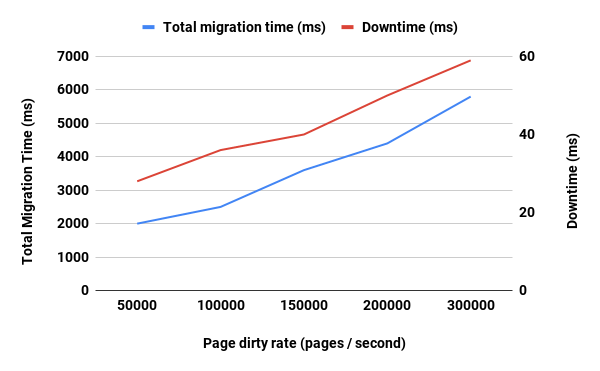
\includegraphics[width=0.5\textwidth]{figures/page_dirty_rate.png}
%\caption{Effect of page dirty rate on total migration time and downtime}
%\label{Effect of page dirty rate on total migration time and downtime}
%\end{figure}

%\begin{figure}[t!]
%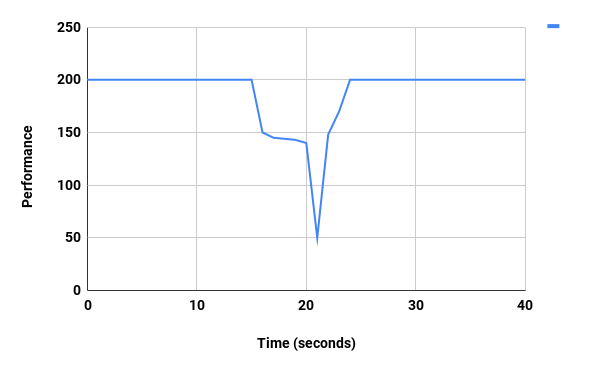
\includegraphics[width=0.5\textwidth]{figures/performance-10Gbps.png}
%\caption{Performance of X benchmark during migration over 10Gbps migration link %bandwidth}
%\label{Performance of X benchmark during migration over 10Gbps migration link bandwidth}
%\end{figure}

%\begin{figure}[t!]
%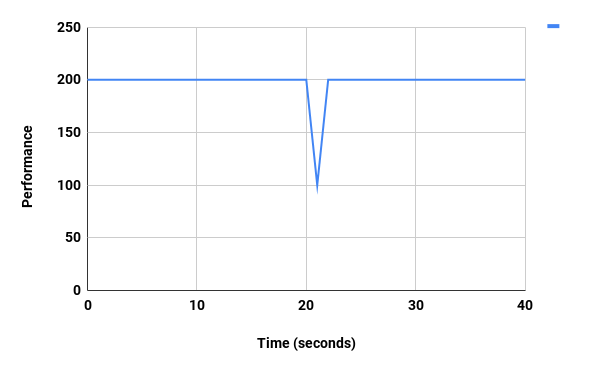
\includegraphics[width=0.5\textwidth]{figures/performance-40Gbps.png}
%\caption{Performance of X benchmark during migration over 40Gbps migration link %bandwidth}
%\label{Performance of X benchmark during migration over 40Gbps migration link bandwidth}
%\end{figure}



\section{Problem Demonstration}
\label{sec:motiv}
%\begin{figure}[t!]
%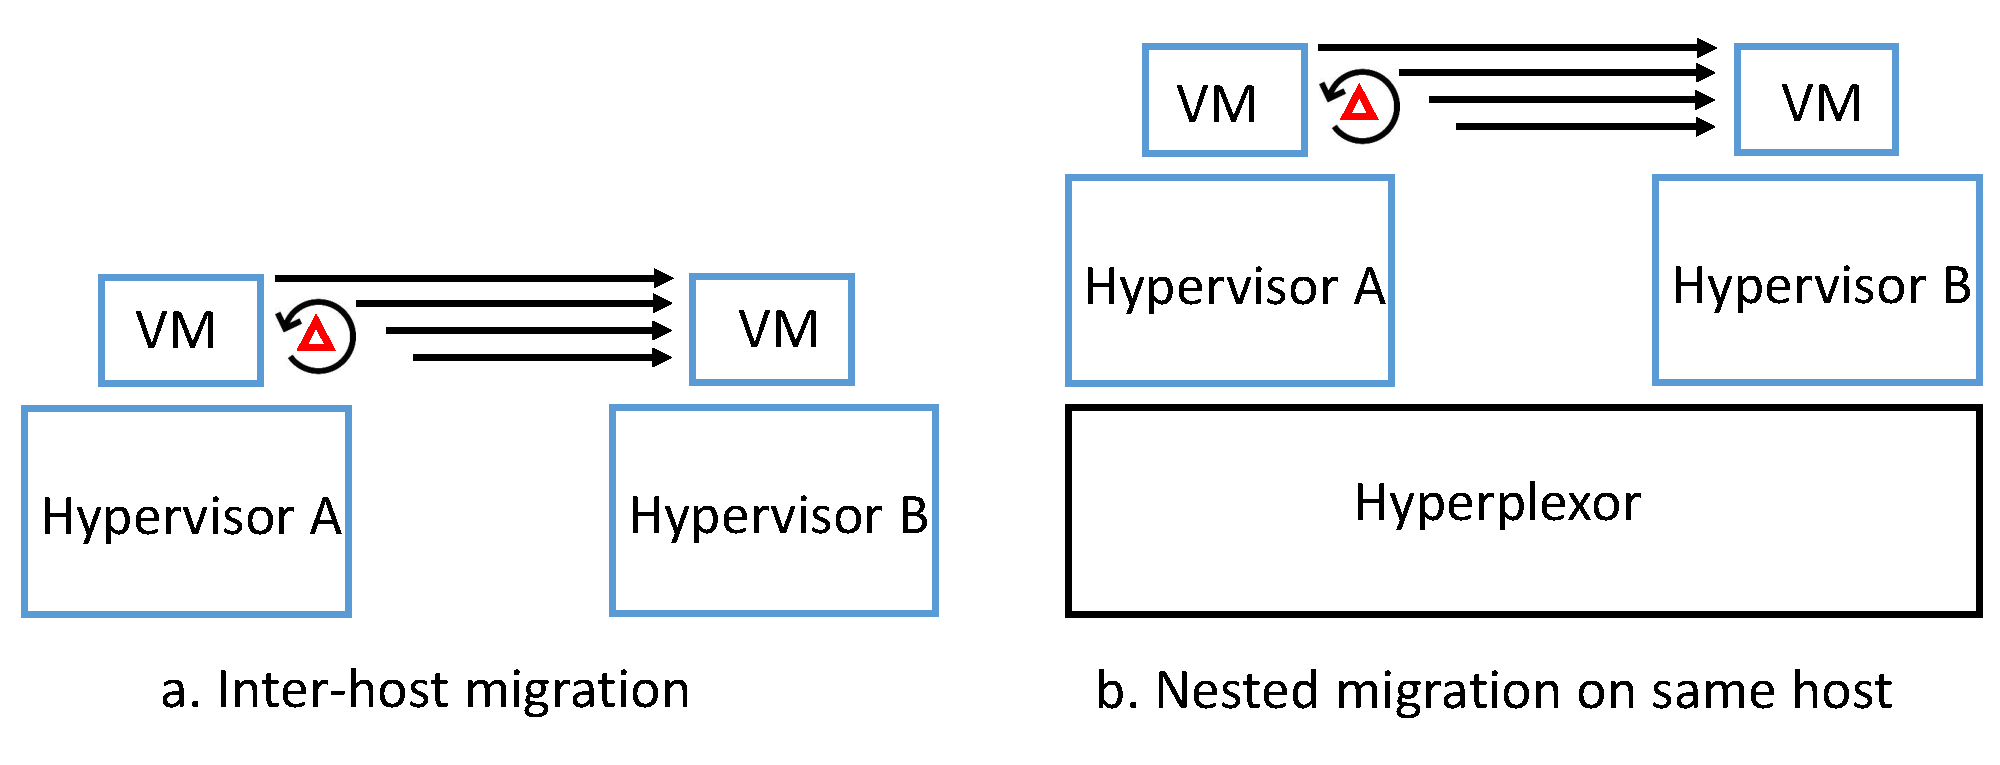
\includegraphics[width=0.45\textwidth]{figures/pre-copy-with-subtitles.pdf}
%\caption{Replacing hypervisor using a. Inter-host migration b. Nested migration on same host}
%\label{fig:motivsetup}
%\end{figure}
In this section, we examine the performance of traditional live migration for hypervisor replacement 
to motivate the need for a faster remapping-based mechanism.

\begin{figure} 
	\centering
	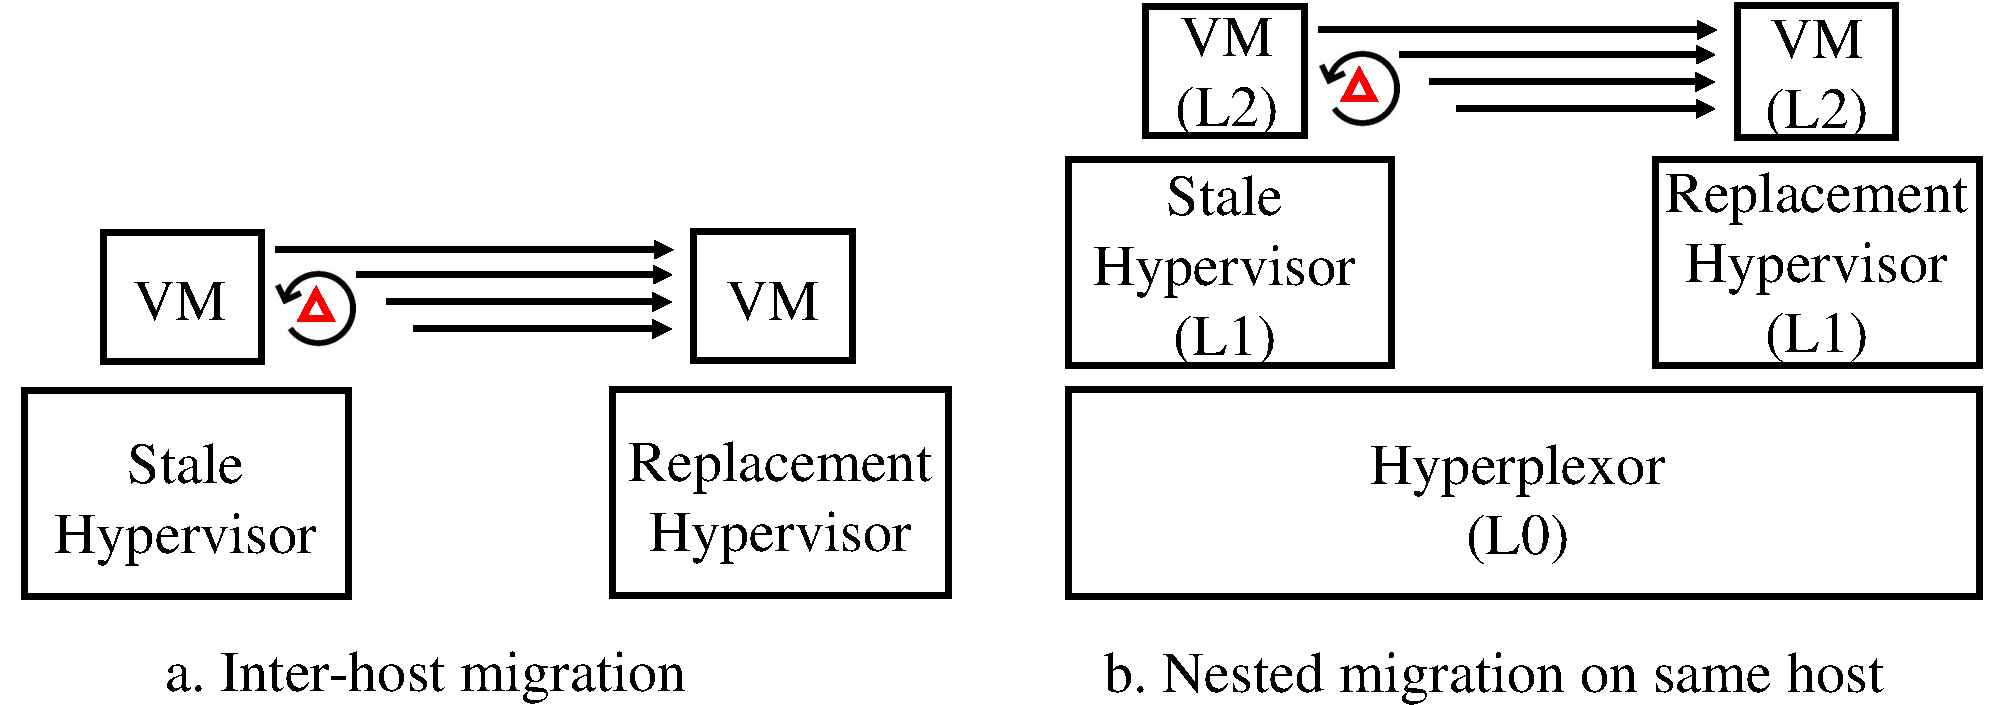
\includegraphics[width=0.45\textwidth]{figures/setups.pdf}
	\caption{Replacing hypervisor in (a) Inter-host setup (b) Nested setup.}
	\label{fig:motivsetup}
\end{figure}

\subsection{Using pre-copy for hypervisor replacement}
%\begin{itemize}[leftmargin=0.15 in]
\para{Inter-Host Live VM Migration:} To refresh a hypervisor, a traditional approach is to live 
migrate VMs from their current host to another host (or hosts) having an updated hypervisor. 
As shown in Figure \ref{fig:motivsetup}a, we can leverage the  state-of-the-art pre-copy live 
VM migration technique. Pre-copy VM live migration consists of three major phases: iterative 
memory pre-copy rounds, stop-and-copy, and resumption.
During the memory pre-copy phase, the first iteration transfers all 
memory pages over the network to the destination, while the VM continues to execute concurrently. 
In the subsequent iterations, only the dirtied pages are transferred. 
After a certain round of iterations, determined by a convergence criteria, the stop-and-copy phase
is initiated, during which the VM is paused at the source and any remaining dirty pages, VCPUs, 
and I/O state are transferred to the destination VM. Finally, the VM is resumed at the destination.

\para{Intra-Host Live VM Migration:} As shown in Figure \ref{fig:motivsetup}b, using nested virtualization, a base hyperplexor at layer-0 (L0) can run deprivileged hypervisors at layer-1 (L1), which control the VMs running at layer-2 (L2). At hypervisor replacement time, the hyperplexor can boot a new replacement hypervisor at L1, and use intra-host live VM migration to transfer VMs from the stale hypervisor to the replacement hypervisor.
%\end{itemize}

%with The objective of HyperFresh is to replace hypervisor beneath the guest with minimal service disruption and performance degradation in guests. The parameters that affect the performance of applications running in the guest are total migration time and downtime. The time from initialization phase to the time when the VM resumes at the destination is the total migration time. Downtime is the time during which the VM remains unresponsive.
%We observed that, live migration of 1GB idle guest using default QEMU's pre-copy takes 12s of total migration time over a 20 Gbps network card. The total migration time is high as QEMU limits the default migration bandwidth to 256Mbps. To compare our results with the best case of QEMU, we modified the pre-copy live migration algorithm. 

\begin{figure*}[h!]
	\centering
	\subfloat[Idle guest]{
		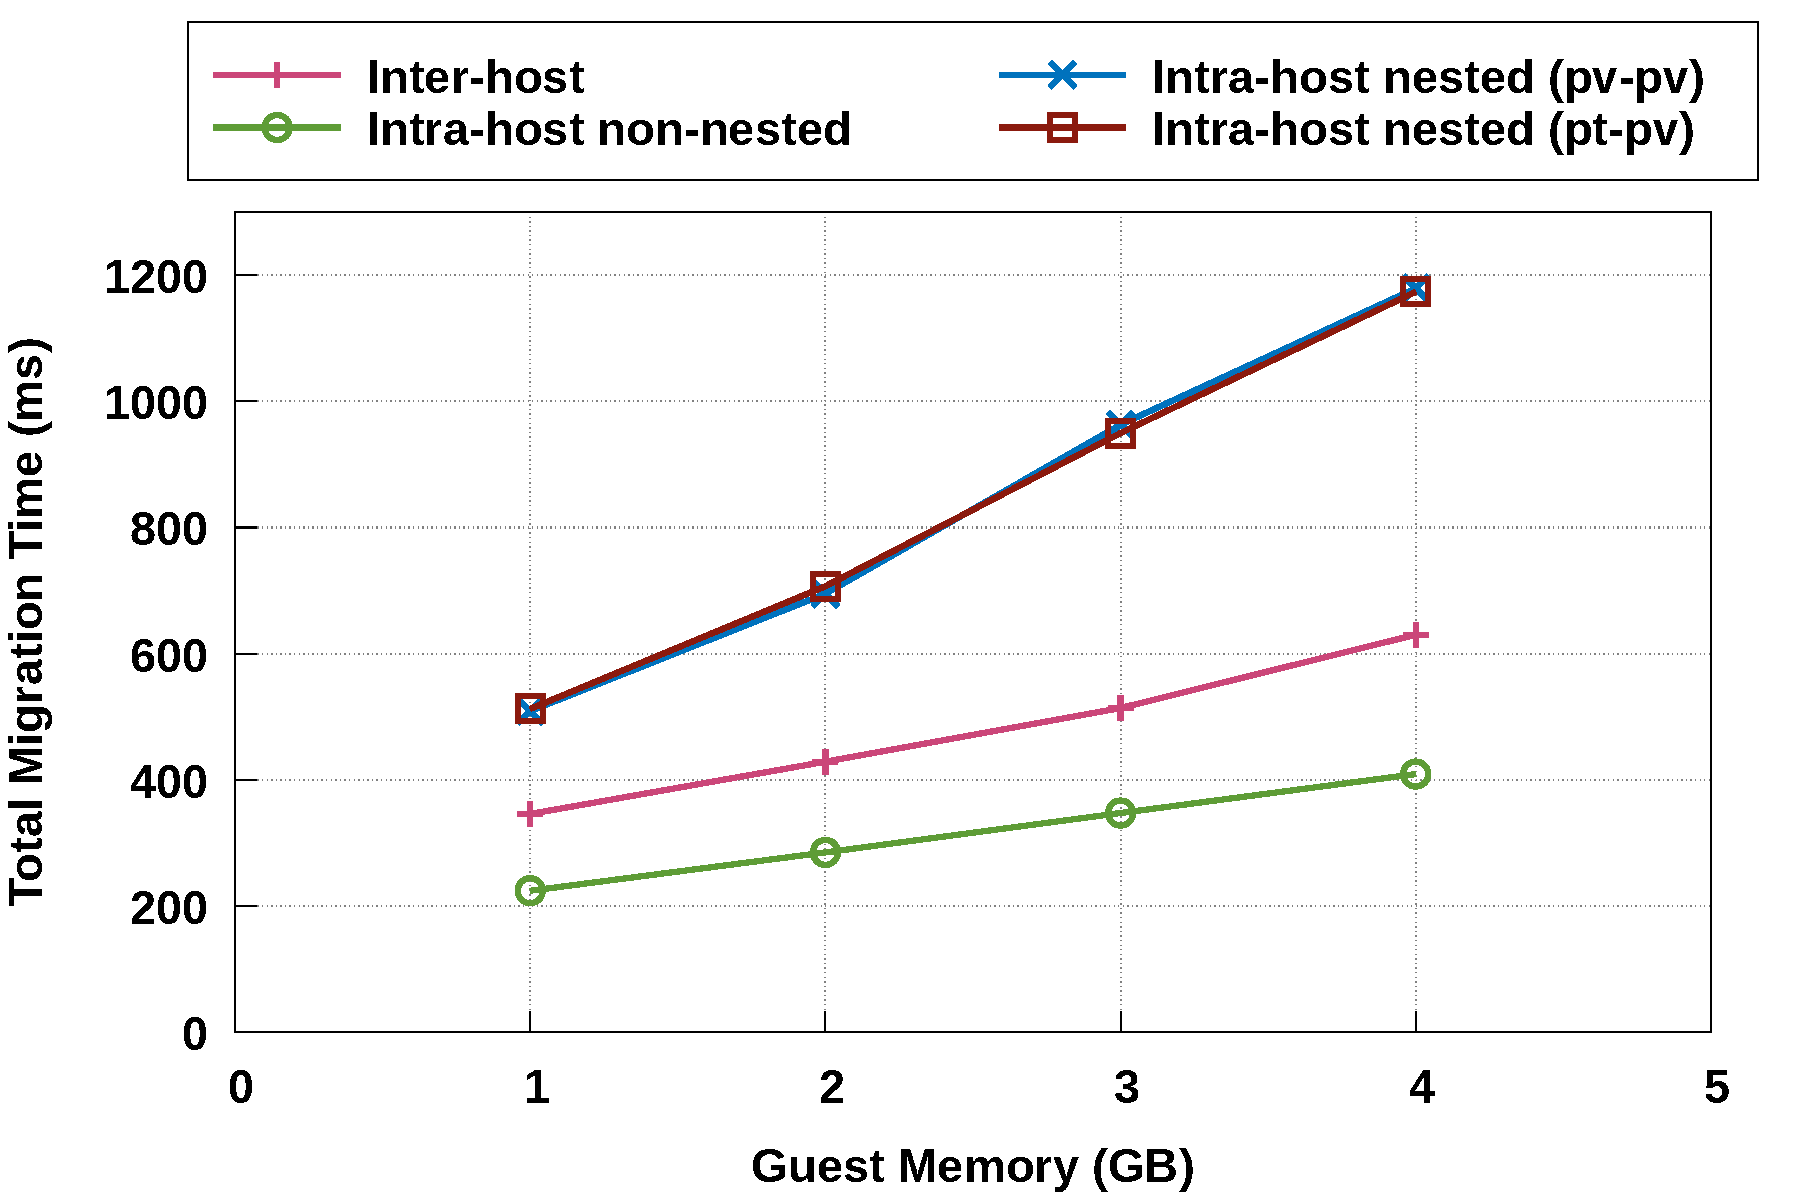
\includegraphics[width=0.48\textwidth]{figures/idle_guest_migration.pdf}}
	\subfloat[Busy guest]{
		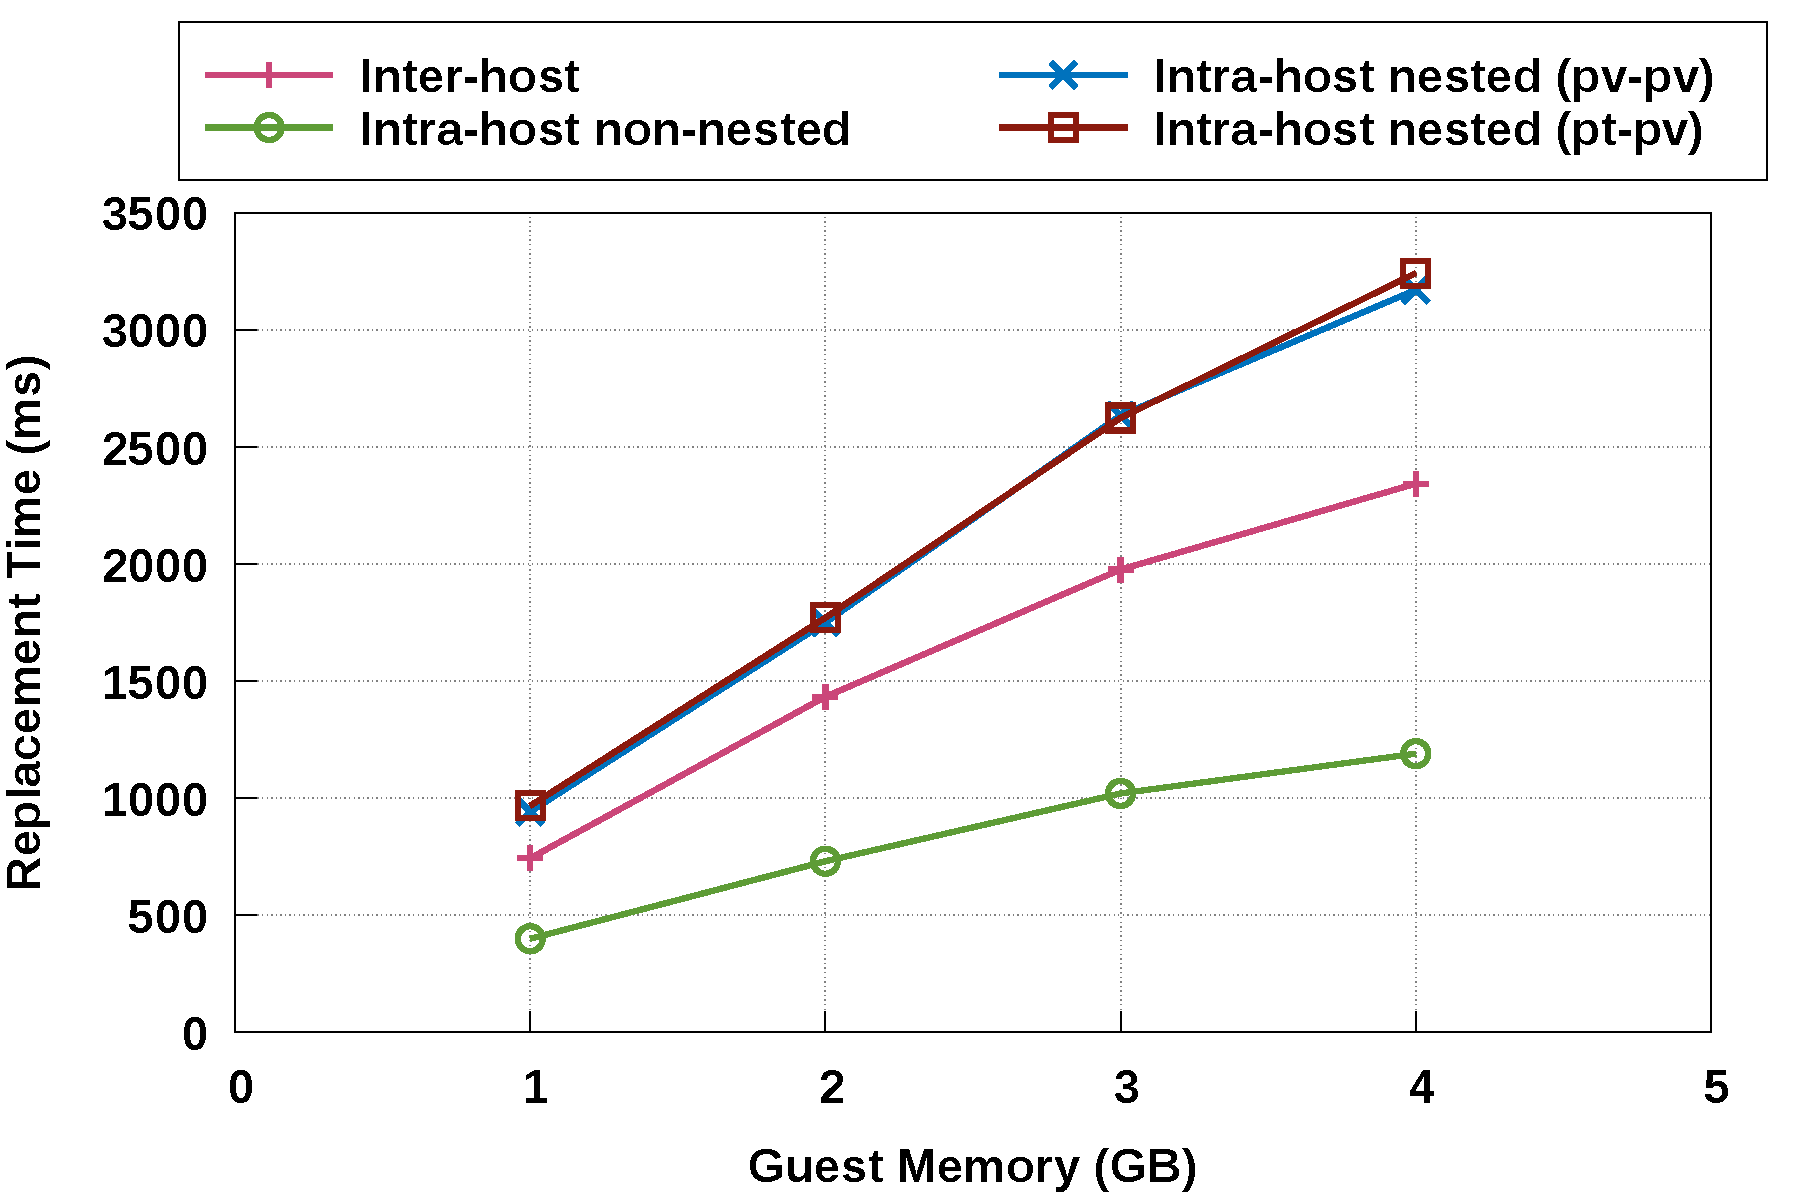
\includegraphics[width=0.48\textwidth]{figures/busy_guest_migration.pdf}}
	\caption{Comparison of hypervisor replacement time between the same and different hosts with nested and non-nested setups.}
	\label{fig:motiv}
\end{figure*}

\subsection{Improving the default pre-copy implementation in KVM/QEMU} 
We observed two performance problems when using the default pre-copy implementation of KVM/QEMU.
So that we can compare our remapping approach with the best case performance of pre-copy implementation, 
we modified the pre-copy implementation as described below. 

First, we observed that the total live migration time for a 1 GB idle VM between two
physical machines connected via a 40 Gbps 
network link was 12 seconds, which was way more than what we expected. 
Upon investigation, we found that, by default, QEMU limits the migration bandwidth to 256 Mbps. 
We modified QEMU to disable this rate limiting mechanism, 
so that the VM's memory can be transferred at full network bandwidth.

Secondly, we observed that when the VM is running a write-intensive workload
then the pre-copy iterations never converge to the stop-and-copy phase.
This was found to be due to an inaccurate convergence criteria
based on the VM's page dirtying rate (the rate at which a VM writes to its memory pages), 
which not only breaks down for write-intensive VMs, 
but also misses opportunities for initiating an earlier stop-and-copy phase 
when the number of dirtied pages in the the last iteration could be low. 

To ensure that the pre-copy rounds converge successfully, we made two additional changes
to QEMU's pre-copy implementation. We placed a hard limit of 20 rounds on the 
maximum number of pre-copy iterations, after which the stop-and-copy phase is initiated.
We also simplified QEMU's default convergence criteria by triggering the
stop-and-copy phase when the number of dirty pages from the prior round is less than 5,000 pages.
The latter change yields a low downtime of less than 5 ms.
%TODO: Kartik: Confirm that the downtime was 5ms.
\footnote{We note that these modifications are meant specifically to improve pre-copy performance in 
our experiments and are not general recommendations for production settings}.


%In addition, to control the downtime and the total migration time for write-intensive workloads, we add the following conditions to move to the {\em stop-and-copy} phase if one of the following conditions is met: (1) The number of dirty pages to be transferred is less than 5000; or (2) If the number of pre-copy iterations exceeds 20. 

%The first condition ensures minimum downtime as the number of pages transferred during last phase is very less. If the workload in the VM is write-intensive, and the rate at which the workload is dirtying the pages is greater than the migration link bandwidth, the migration never converges. To ensure that the migration completes successfully, we restrict the number of pre-copy iterations to 20. After 20 iterations the VM moves to stop and copy phase.

%Guest Memory (GB)	Inter-host	Intrahost non-nested	Intrahost nested (pv-pv)	Intrahost nested (pv-pt)
%1	346.2	224.4	509.2	512.6
%2	429	    285.2	695	    707
%3	514	    347.6	963	    949.6
%4	630.2	409.4	1179	1173.6

%\begin{figure}[t!]
%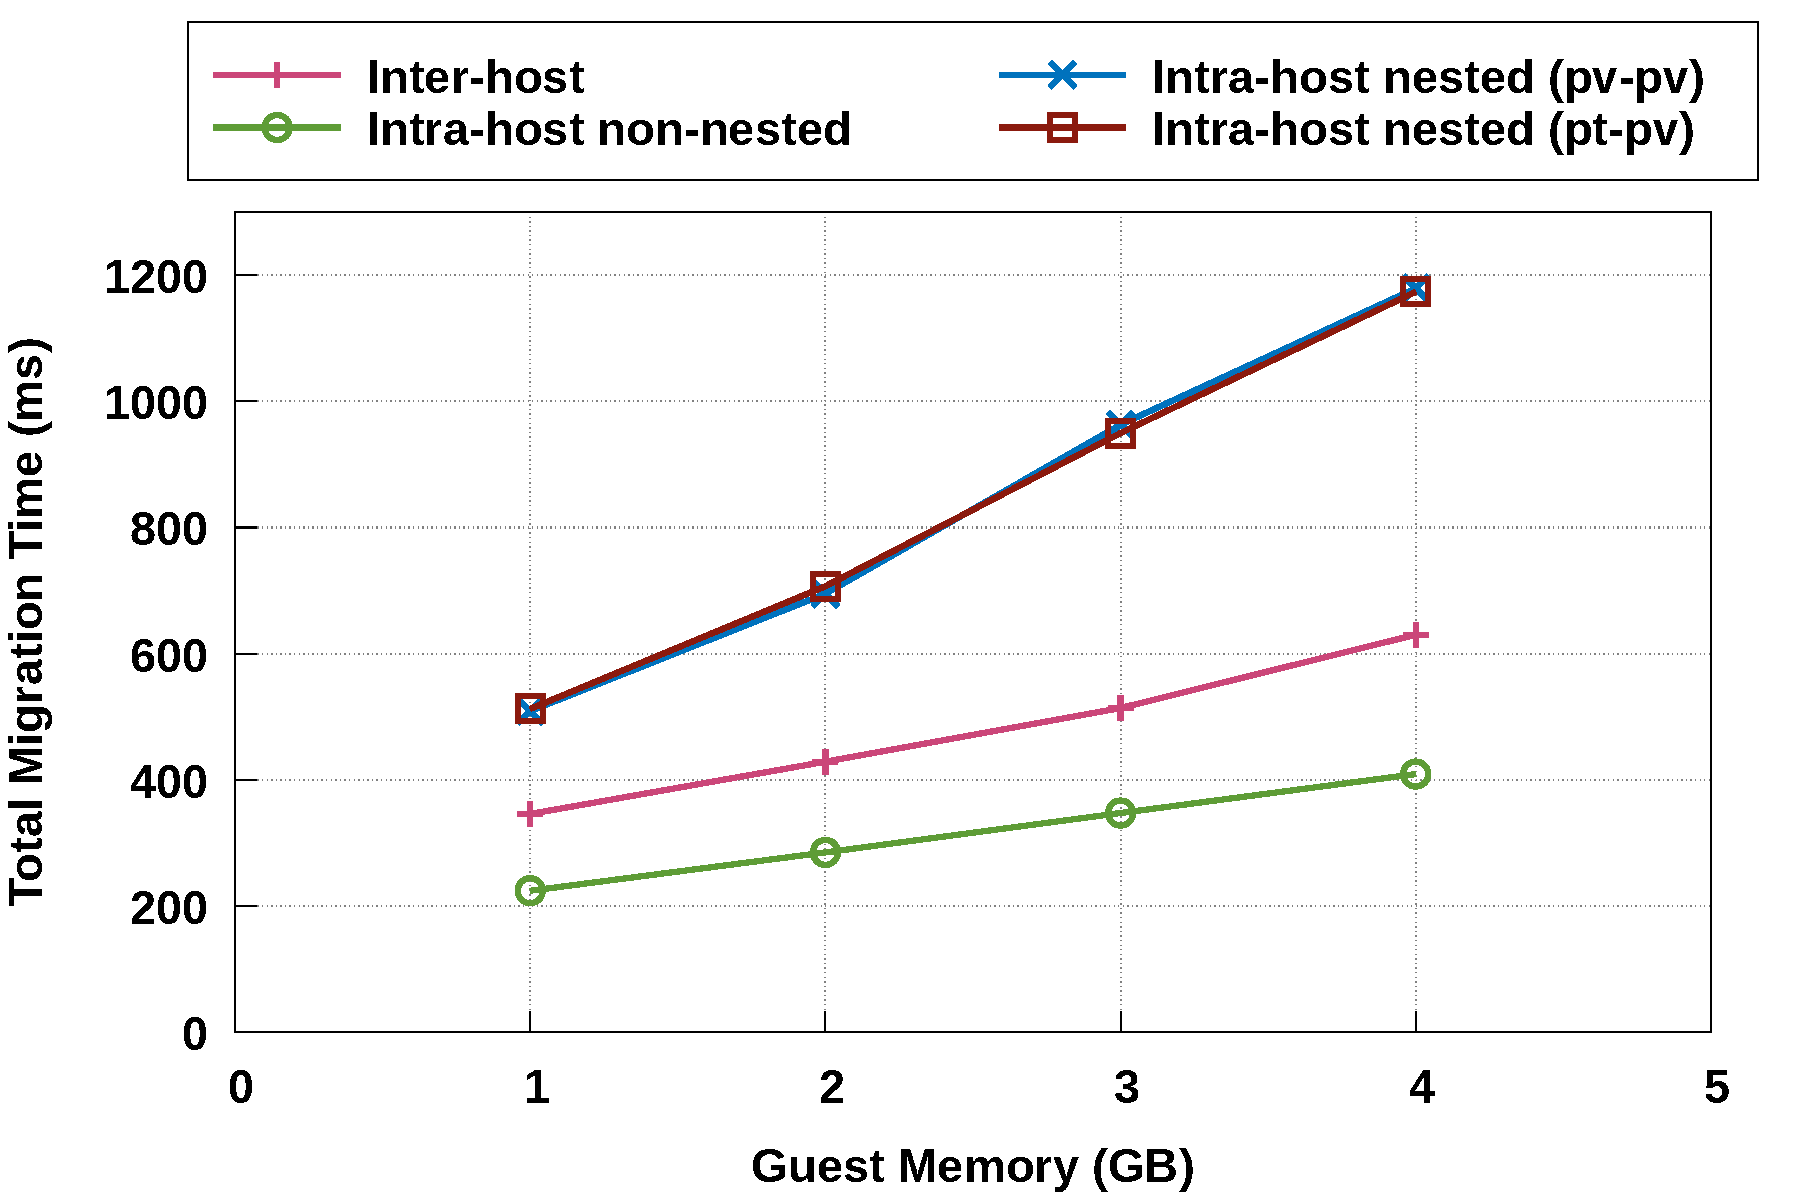
\includegraphics[width=0.45\textwidth]{figures/idle_guest_migration.pdf}
%\caption{Idle guest: Comparison of hypervisor replacement time between the same and different hosts with nested and non-nested setup.}
%\label{fig:motivid}
%\end{figure}

%Guest Memory (GB)	Inter-host	Intrahost non-nested	Intrahost nested (pv-pv)	Intrahost nested (pv-pt)
%1	743.6	399.6	942.4	967.4
%2	1433	730.6	1750	1770.6
%3	1975.8	1020	2634	2623.2
%4	2342.6	1190	3170	3241.6

%\begin{figure}[t!]
%  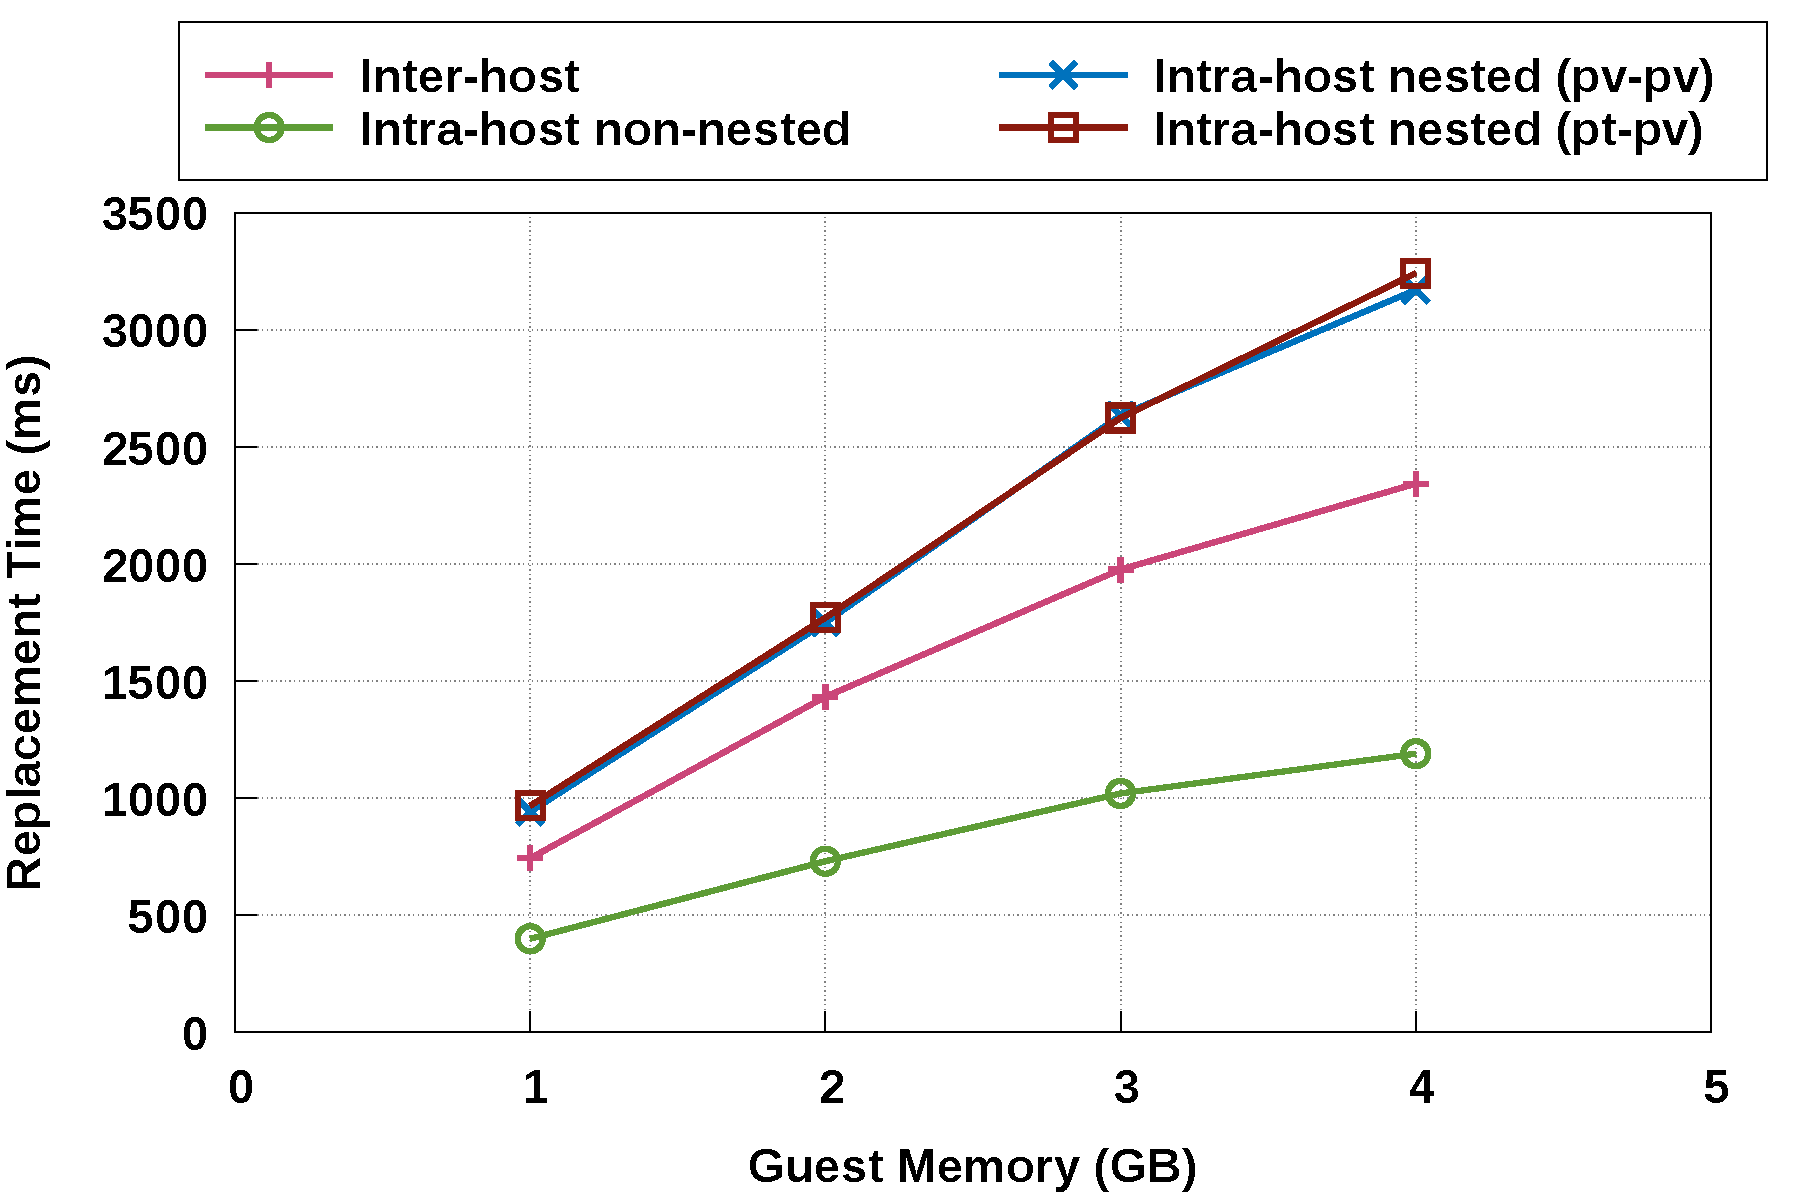
\includegraphics[width=0.45\textwidth]{figures/busy_guest_migration.pdf}
%  \caption{Busy guest: Comparison of hypervisor replacement time between the same and different hosts with nested and non-nested setup.}
%  \label{fig:motivbz}
%\end{figure}

%\begin{figure}
%	\centering
%	\subfloat[Idle guest]{
%		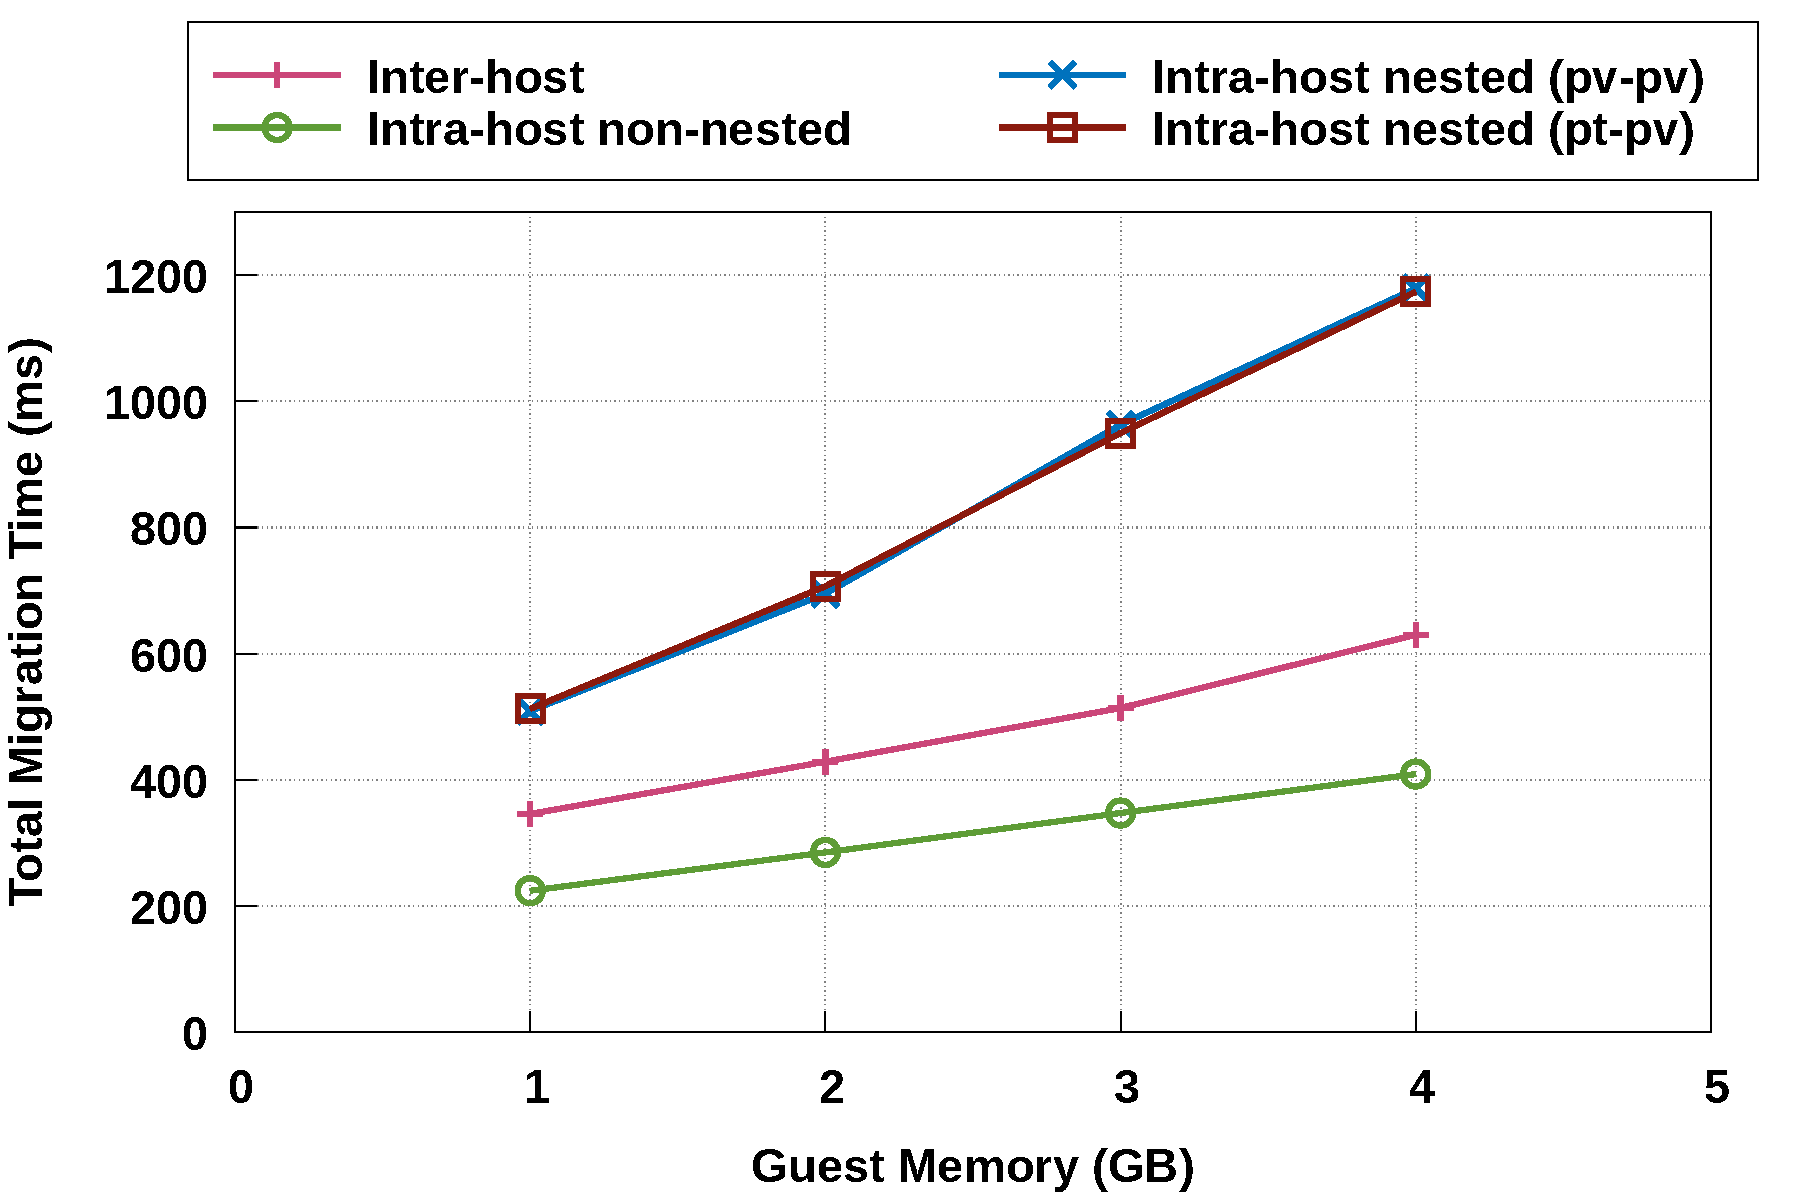
\includegraphics[width=.235\textwidth]{figures/idle_guest_migration.pdf}}
%	\subfloat[Busy guest]{
%		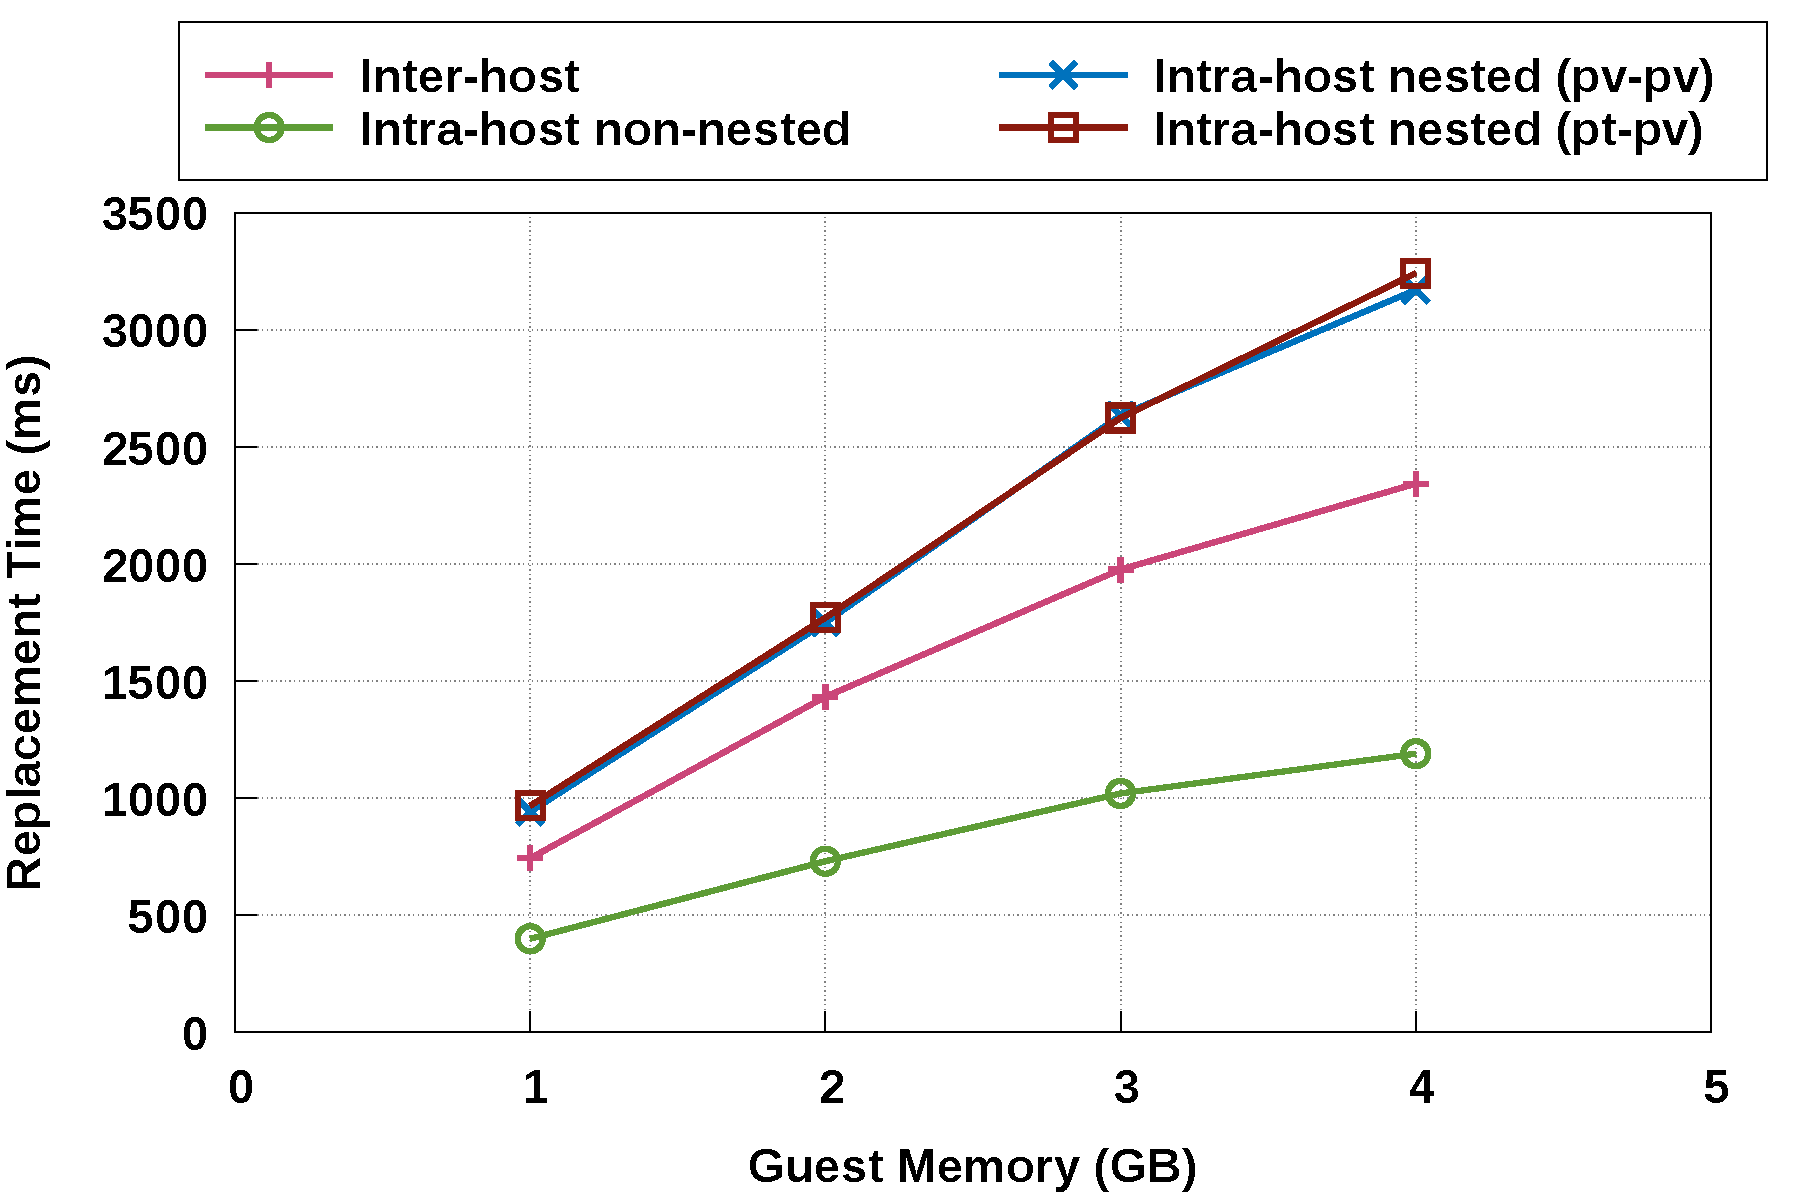
\includegraphics[width=.235\textwidth]{figures/busy_guest_migration.pdf}}
%	\caption{Comparison of hypervisor replacement time between the same and different hosts with nested and non-nested setup}
%	\label{fig:motivid}
%\end{figure}

%\begin{figure}
%	\centering
%	\subfloat[Idle guest]{
%		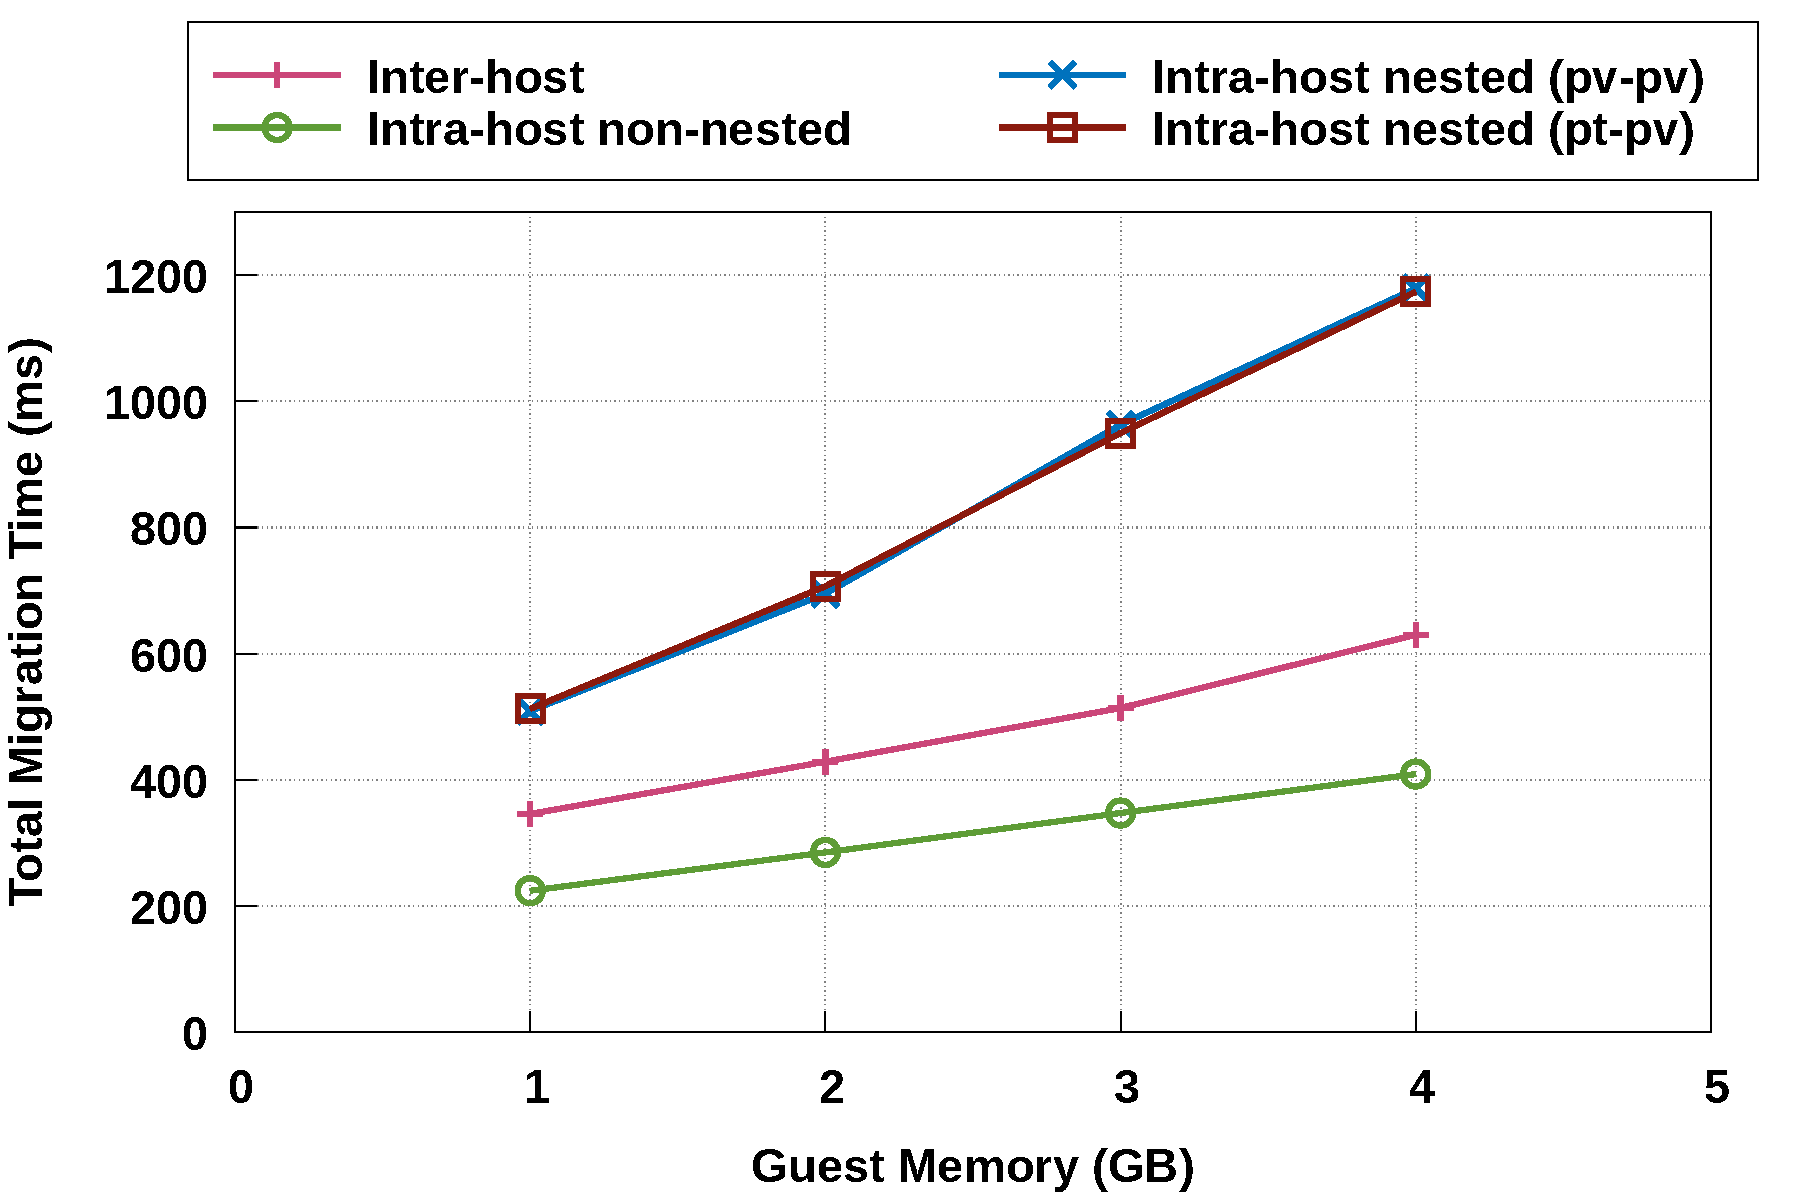
\includegraphics[width=.235\textwidth]{figures/idle_guest_migration.pdf}}
%	\subfloat[Busy guest]{
%		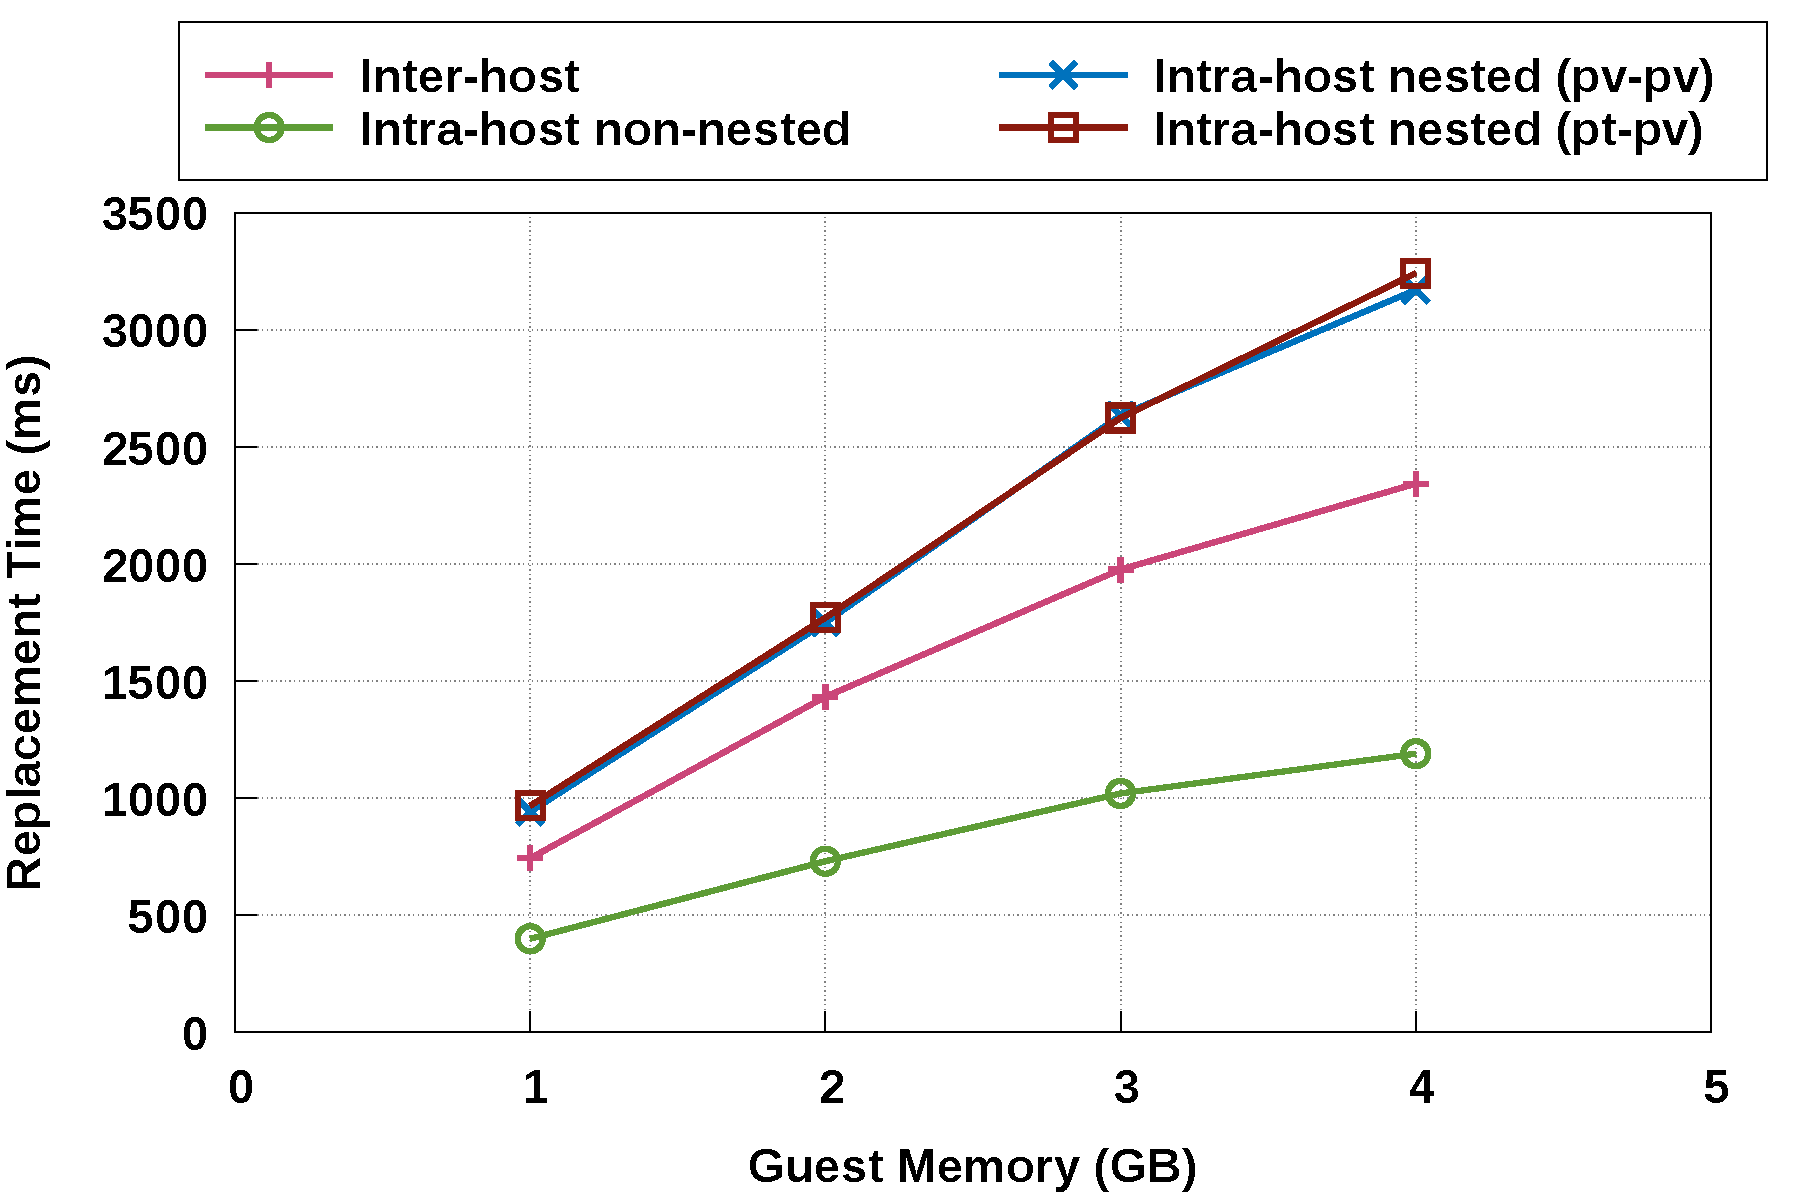
\includegraphics[width=.235\textwidth]{figures/busy_guest_migration.pdf}}
%	\caption{Replacement time comparison}
%	\label{fig:rt_motivation}
%\end{figure}

\subsection{Analysis of pre-copy performance for hypervisor replacement}
With the above optimizations to QEMU's default pre-copy live migration, 
we analyzed the total migration time, which also represents the time taken 
for hypervisor replacement operation.  We analyzed the following four configurations:
\begin{itemize}[leftmargin=0.15 in]
\parskip 0mm
\itemsep 0mm
\item {\bf Inter-host:} where a VM is migrated between two physical machines, as in Figure~\ref{fig:motivsetup}a. The source machine runs the stale hypervisor and the destination machine runs the new hypervisor.
\item {\bf Intra-host nested (pv-pv):} where the VM is migrated between two {\em co-located nested hypervisors}, as in Figure~\ref{fig:motivsetup}b. The source L1 runs the stale hypervisor and the destination L1 runs the new hypervisor. The network interfaces of both L1 hypervisors and their L2 VMs are configured as para-virtual {\em vhost-net} devices~\cite{vhost-net}.
\item {\bf Intra-host nested (pt-pv):} Same configuration as the above case, except that the both L1 hypervisors are configured to use pass-through network interfaces via virtual functions configured in the physical NIC.
\item {\bf Intra-host non-nested:} This is a baseline (and somewhat unrealistic) migration scenario where a single-level non-nested VM is migrated within the same host into another VM instance. This case helps us measure the intra-host live migration performance if there were no overheads due to nested virtualization and network interfaces (since source and destination QEMU processes communicate via the loopback device).
\end{itemize}
The experiments were conducted using machines having 10-core Intel-Xeon 2.2 GHz processors with 32GB memory 
and 40 Gbps Mellanox ConnectX-3 Pro network interface. 

Figure~\ref{fig:motiv}a plots the total migration time for an 
idle VM when the VM's memory size is increased 
from  1 GB to 4 GB. 
Figure~\ref{fig:motiv}b plots the total migration time for a busy VM
where the VM runs a write-intensive workload in the VM. Specifically, the 
write-intensive workload allocates a certain size of memory region and writes a few 
bytes to each allocated page at a controllable dirtying rate. 
The allocated memory size is 80\% of the VMs memory,  from 800 MB for a 1 GB VM to 3,200 MB for a 4 GB VM. 
The dirtying rate is set to 50,000 pages per second.

First we observe that in all the cases, as the VM size increases, 
the total migration time increases, because more memory pages must be transferred 
over a TCP connection for larger VMs. The migration times range from as low
as several hundred milliseconds for idle VMs to more than 3 seconds for 
busy write-intensive VMs. Since pre-copy retransmits dirtied pages from 
previous iterations, write-intensive VMs take longer to migrate.

The second surprising observation was that the {\em Inter-host} configuration  
for migrating a non-nested VM was faster than the {Intra-host}
configuration for migrating a nested VM. Replacing the para-virtual
{\em vhost-net} interface for the L1 hypervisor in the {\em Intra-host nested (pv-pv)} configuration with 
a pass-through interface in the {\em Intra-host nested (pt-pv)} configuration did not produce any noticeable
reduction in total migration time. 
%(However we did observe a reduction in 
%CPU utilization when pass-through I/O is used for the L1 hypervisor in the {\em pt-pv} case.)
To verify that this worse performance was caused by nesting overheads,
we carried out the {\em Intra-host non-nested} live migration described above. 
As expected, this fourth configuration performed better than the {\em Inter-host} 
configuration, confirming that nesting overheads indeed adversely affect 
intra-host VM migration.

Nevertheless, even in the ideal (though unrealistic) 
case represented by the {\em Intra-host non-nested} setting, 
traditional pre-copy migration takes between 0.4 seconds (for idle VM case)
to more than 1.19 seconds (for busy VM case) to migrate a single 4 GB busy VM. 
When multiple VMs must be relocated for hypervisor replacement, these 
times are bound to increase. We consider this performance unsatisfactory
for simply relocating VMs within the same host.

In summary, using intra-host pre-copy live migration for hypervisor 
replacement is expensive in terms of total migration time, network
overheads, and its affect on VM's performance. 
This motivates us to develop a much faster hypervisor replacement
technique based on memory remapping that does not involve copying of 
VM's memory pages within the same host. In the following sections,
we present our approach and show that our memory remapping-based
technique can achieve sub-10ms live hypervisor replacement times for VMs
and sub-second live OS replacement times for containers.

%During migration, the performance of VMs being migrated could be negatively impacted.  In addition, the large traffic generated during migration may impact other unrelated VMs sharing the same network infrastructure. These motivate us to seek a new technique for {\em fast} hypervisor/OS replacement. 

%-------------

%\para{Idle Case.} In \fref{fig:motivid}, we observe that, in the pre-copy live migration scenario, as the memory size of an idle VM increases, the total migration time increases accordingly. For example, the migration time increases from 346.2 ms for a 1 GB VM to 630.2 ms for a 4 GB VM for inter-host migration. Such an increase in total migration time is due to more memory transferred in pre-copy iteration rounds. 
%
%In contrast, we measured the migration time in the ``intra-host'' live migration scenario under nested virtualization.  We consider two typical configurations: (1) both L1 hypervisors and L2 VMs use the para-virtual driver; and (2) L1 hypervisors use  pass-through devices whereas L2 VMs use para-virtual driver. As shown in \fref{fig:motivid}, in comparison with the inter-host pre-copy scenario, we have the similar observation: as the memory size of the idle VM increases, the migration time also increases. Using either configuration 1 or 2, the ``intra-host'' case leads to higher total migration time compared to ``inter-host'' case. 
%%--- slightly higher when the memory size of the idle guest is 4 GB. 
%Though, with configuration 2, we do not observe much difference in terms of total migration time in comparison with configuration 1, we do observe lower CPU usage, as I/O pass-through eliminates the software overhead for L1.
%
%As hypervisor replacement occurs on the same host in our solution, we also measure the cost to migrate the guest on the same host. In \fref{fig:motivid}, the time spent in migrating a non-nested VM on the same host is still significantly high as the memory is still copied in multiple rounds. 
%
%%We also measure the total migration time to migrate a nested guest from one hypervisor to another on the same host. We consider two different configurations to measure migration of nested guest. In the first case, the hypervisor and the guest both use para-virtual driver to transmit the network packets. In the latter case, the hypervisor uses a pass-through device whereas the guest uses a para-virtual driver. 
%In \fref{fig:motivid}, the total migration time for the nested VM increases in both the cases compared to intra-host non-nested case due to the overhead induced by nested virtualization. In the figure, we see that these two configurations give almost the same performance. The difference in para-virtual/para-virtual(pv-pv) and pass-through/para-virtual(pt-pv) configuration is the CPU utilization on the host which is discussed in more detail in the design and evaluation sections.
%
%\para{Busy Case.} We run a write-intensive workload in the VM. More specifically, the write-intensive workload allocates a certain size of memory and dirties the memory by writing few bytes to the allocated memory at a controllable dirty rate. In the experiments, we vary the workload memory from 800 MB for a 1GB VM to 3200 MB for a 4 GB VM, which is 80\% of the memory and set the dirty rate to 50,000 pages per second. We migrate the VM after the given workload size is dirtied. 
%
%\fref{fig:motivbz} shows that, in all cases, the total migration time increases as the memory of the workload increases. It takes significant time to copy the working set memory over the network for inter-host migration (e.g., 2,342.6 ms for a 4 GB VM). 
%Again, the ``intra-host'' migration case without nested virtualization spends less time in migrating the VM, in comparison with the ``inter-host'' case.
%%a significant amount of memory copied on the same host. 
%The ``intra-host'' migration case with nested virtualization spends more time compared to the ``intra-host'' migration  without nested virtualization because of the nested virtualization overhead. 
%%Such overhead can be mitigated, if we use pass-through I/O devices for L1 hypervisor. 
%-------------


%The performance of the guest degrades considerably as the dirty page rate approaches the migration link bandwidth.
%The two factors that significantly affect the migration are page dirty rate and migration link bandwidth. The increase in dirty page rate increases the number of memory transfer rounds over the network. However, the downtime remains almost constant with varying dirty page rate as the number of pages transferred in the stop and copy phase is always less than 5000. In Fig. 2, a 2GB guest running a write-intensive application dirties memory at specified rate (pages / second). The migration link bandwidth is fixed to 1Gbps. We observe that the total migration time increases from abc to xyz as the page dirty rate increases. The downtime remains as low as 5ms. 

%If the migration link bandwidth increases, the total migration time and downtime decrease. A guest configured with 2GB memory and runs a memory intensive workload, zeusmp, a SPEC CPU2017 benchmark. The total migration time and downtime are measured as the migration link bandwidth is varied from 10Gbps to 40Gbps. From Fig. 3 and Fig. 4, the total migration time and downtime decrease as the migration link bandwidth increases. For a 10Gbps migration link bandwidth, the performance of the application running in the guest degrades due to high total migration time and downtime compared to 40Gbps migration link bandwidth.

%Setting the migration link bandwidth to a higher value improves the migration time but at the same time it generates huge network traffic. If the migration bandwidth is fixed to a lower value, the migration time increases and it affects the performance of the applications in the guest.

%\input{background.tex}
\section{\arch for Hypervisor Replacement}
In this section, we introduce the design and implementation of \arch for 
live hypervisor replacement, followed by live OS replacement 
in the next section. 
The key idea behind \arch is as follows: Instead of copying the memory 
of VMs from the stale hypervisor to the co-located replacement hypervisor, 
\arch transfers the ownership of VMs' physical memory pages via page table remapping. 
Such memory ownership relocation is fast and leads to sub-10ms live hypervisor 
replacement. In addition, \arch includes optimizations to further mitigate 
nesting overhead during normal execution of VMs.
We first introduce memory translation under nested virtualization, 
followed by hyperplexor-based hypervisor switching, and finally 
optimizations to mitigate nesting overheads.


%The key design goals of the proposed work are transparency and minimum 
%service disruption in guests. The architecture of live hypervisor replacement
%is shown in Figure~\ref{fig:arch}. Using nested virtualization, the hypervisors at L1 and unmodified guests are run on thin hyperplexor at L0. Using SR-IOV, a single PCI device or physical function is presented as multiple virtual functions to hypervisors to reduce the performance overhead in guest due to nested virtualization. Upon a migration event, an updated hypervisor is first started on thin hyperplexor. The updated hypervisor then replaces the aged hypervisor by co-mapping the memory of guest. The hyperplexor transfers the memory mappings using grant table mechanism where the  guest page frames are mapped to the updated hypervisor followed by unmapping of memory from the aged hypervisor. The completion of hypervisor replacement is marked by pausing the guest and transferring the vCPU and I/O states to the updated hypervisor.  

\begin{figure}[t!]
 	  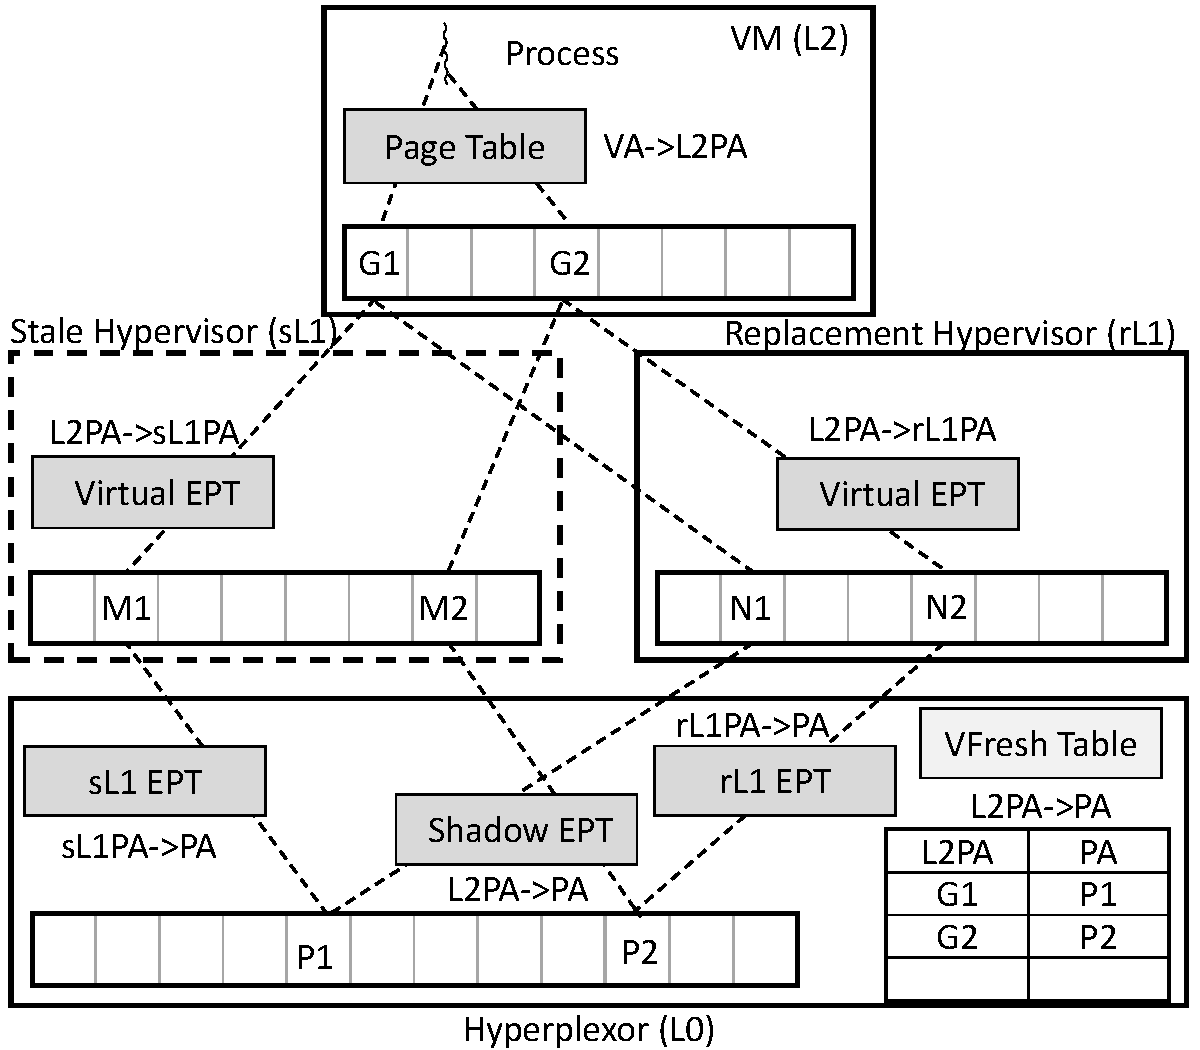
\includegraphics[width=0.45\textwidth]{figures/vfresh-table.pdf}
  \caption{Memory translations for hypervisor replacement.}
  \label{fig:mapping}
  %\includegraphics[width=15cm,height=6cm,keepaspectratio]{architecture__1_.jpg}
\end{figure}

\subsection{Memory Translation for Nested Virtualization}
In native execution mode (without virtualization), a page table stores the mappings between 
the virtual addresses (VA) of a process to its physical addresses (PA) 
where memory content actually resides. When a VA is accessed by 
a process, the hardware memory management unit (MMU) uses the page table 
to translate the VA to its PA.

In single-level virtualization, an additional level of address translation 
is added by the hypervisor for virtualizing the memory translations for VMs. 
The page table of a process running on a VM stores the mappings from the guest 
virtual addresses (GVA) of a process to the guest physical addresses (GPA),
which is the virtualized view of memory seen by the VM. 
The hypervisor uses another page table, called the extended page table (EPT) 
to map GPA to its physical addresses (PA). 
As with traditional page tables, an EPT is constructed incrementally upon page faults.
As a VM tries to access previously unallocated GPA, EPT violations are generated, 
like page faults for a process. 
These faults are processed by the hypervisor which allocates a new physical page 
for the faulting GPA. 

In nested virtualization, as shown in \fref{fig:mapping}, 
three levels of translations are needed. A process's virtual address is translated to the GPA 
of the layer-2 VM (labeled L2PA). 
An L2PA is translated to the guest physical address of the L1 hypervisor (L1PA) using a
{\em virtual EPT} for the layer-2 VM maintained by the L1 hypervisor. Finally, 
the L1PA is translated to the physical address of the host (PA) using the L1 hypervisor's EPT  
maintained by the hyperplexor at L0. Since, the MMU can translate only two levels 
of memory mappings, the hyperplexor at L0 combines the virtual EPT at L1 and the EPT at L0 to 
construct a {\em Shadow EPT} for every L2 VM.
The MMU uses the process page table in the L2 VM and the shadow EPT at L0 to translate a 
process VA to its PA. The shadow EPT is updated whenever the corresponding virtual EPT in L1 
and/or the EPT in L0 are updated.
 
\subsection{Hypervisor Replacement Overview}
We now present an overview of the hypervisor replacement mechanism followed by  low-level details.
Consider a VM that initially runs on the stale L1 hypervisor which in turn runs on the 
thin L0 hyperplexor.
To replace the stale hypervisor, the hyperplexor creates a new replacement L1 hypervisor (with pre-installed updates) 
and transfers the ownership of all L2 VMs' physical pages to this replacement hypervisor.

The page mappings from an L2 VM's guest physical address (L2PA) to the physical memory (PA) are
available in the shadow EPT of the L2 VM. 
Ideally, the hyperplexor could accomplish the L2 VM's relocation
simply by reusing the shadow EPT, albeit under the replacement hypervisor's control.
However, since the shadow EPT is the result of combining a nested
VM's virtual EPT in L1 and L1's own EPT in L0, these two intermediate mappings 
must be accurately reconstructed in the new address translation path via 
the replacement hypervisor. 

To accomplish this reconstruction, the replacement hypervisor must coordinate 
with the hyperplexor.
It does so by preparing a skeletal L2 VM to receive each incoming L2 VM
and reserves unallocated L1 page frame numbers in its guest-physical address space (L1PA) 
where the incoming VM's pages will be mapped. 
The replacement hypervisor then communicates the identity of these reserved page frames 
in L1PA to the hyperplexor (via a hypercall), so that the hyperplexor
can map these reserved page frames to the incoming L2 VM's existing physical pages.
Note that the reserved L1 page frames in the replacement hypervisor may not be the same as 
that in stale hypervisor as shown in \fref{fig:mapping}. 

The transfer of execution control is then  performed as follows.
The L2 VM's execution is paused at the stale hypervisor
and its execution state (consisting of all VCPU and I/O states) 
are transferred to the replacement hypervisor's control, which then resumes execution 
of the L2 VM. This switch over operation can be accomplished quickly 
(sub-10ms in our prototype) since no memory content is copied during this step.
Finally, once the control of the L2 VM is transferred to the replacement hypervisor, 
the stale hypervisor can unmap the L2 VM's  memory from its address space and be safely deprovisioned. 

As the relocated L2 VM begins execution on the replacement hypervisor,
it generates page faults against its memory accesses.
The entries in the new intermediate mapping tables (the virtual EPT and replacement hypervisor's 
L1 EPT) are populated on-demand to reflect the original physical 
pages used by the L2 VM under the stale hypervisor. 
In other words, the shadow EPT reconstructed for the relocated
VM ends up being identical to its erstwhile shadow EPT used under the stale hypervisor, while 
the new intermediate mapping tables are correspondingly adjusted.
We nest describe low-level details of \arch implementation.



\subsection{Implementation Details} 
We developed a prototype of \arch using the KVM/QEMU virtualization platforms with Linux kernel 
version 4.13.0 and QEMU version 2.9.0. KVM is a linux kernel module which is responsible for 
core hypervisor functionalities. QEMU is a user space process that manages VM control operations,
including live migration, and emulates its I/O operations. The VM runs unmodified Linux kernel 
version 4.13.0 and uses para-virtual I/O devices.
Our hypervisor replacement solution was implemented by modifying QEMU's live migration mechanism, besides
modifications to KVM to implement page remappings described above. 

Different from QEMU's live migration, 
\arch's hypervisor replacement operation only involves the transfer of VCPU and I/O state of the VM. 
Since the relocation of L2 VM's memory pages is performed 
out of the critical path of hypervisor replacement, we modified QEMU's live migration
to disable dirty page tracking, transfer of page contents via pre-copy iterations, and
also the transfer of residual dirty pages during the stop-and-copy phase of live migration. 
The VCPUs are paused only during the stop-and-copy phase which results in very low hypervisor 
replacement time.

\subsubsection{The \arch Table}
In KVM's current implementation, the L2 VM's shadow EPT cannot be easily transferred 
from the stale hypervisor to the replacement hypervisor.
Hence, our hyperplexor implementation constructs a parallel table, which we call the {\em \arch table},
to store a copy of the L2-to-physical page mapping information contained in the shadow EPT.
This \arch table is used for reconstructing the same L2PA-to-PA page mappings for 
the relocated VM upon EPT violations.

To construct the \arch table, the hyperplexor needs a list of L2-to-L1 page mappings 
of the VM from the stale hypervisor, using the virtual EPT table. 
% as listed in Table \ref{tab:api}. 
The stale hypervisor invokes a \texttt{hypercall\_put} hypercall multiple times
to pass a complete list of L2-to-L1 page mappings 
of the VM to the hyperplexor. For each received L2-to-L1 page mapping, the hyperplexor translates 
the L1 page number to the physical  page number using the EPT table at L0, and inserts 
the corresponding L2-to-physical page mapping into the {\em \arch table}. 

To relocate the ownership of a L2 VM's memory to the replacement hypervisor, the hyperplexor
needs  the list of L2-to-L1 page mappings of the newly created skeletal VM from the replacement hypervisor.
The replacement hypervisor invokes another \texttt{hypercall\_map} hypercall multiple times
to pass these mappings to the hyperplexor. For each received L2-to-L1 page mapping, the hyperplexor 
(1) looks up the {\em \arch table} to find the L2-to-PA mapping with the L2 page number 
as the key; and (2) installs the L1-to-PA page mapping in the replacement hypervisor's 
EPT table. More specifically, \arch translates each L1 guest frame number to its  host virtual address (HVA), 
installs the HVA-to-PA page mapping in the page table of the VM's QEMU process, and at last invalidates the 
corresponding entry in the EPT table, which is reconstructed later upon an EPT  fault.
Also, to clear any pre-existing GFN mappings of the replacement hypervisor, the hyperplexor flushes 
the entries in TLB and page table of QEMU, before resuming the relocated VM.

%TODO: Kartik: Spoorti, The following details can be included in your dissertation. Its too low for the paper.
%\para{Memory Relocation:}
%The source VM's QEMU makes an IOCTL to request current KVM hypervisor to pin the VM pages in memory during the boot time. Hypervisor uses memory slots to get the VM frame numbers (GFNs) of the VM and translates all the VM GFNs to hypervisor GFNs. KVM then transfers the VM GFNs and hypervisor GFNs mapping information to the hyperplexor using \texttt{hypercall\_set} hypercalls. The hyperplexor pins the pages in memory using the hypervisor GFNs. Hyperplexor creates the \arch table with VM GFN to physical frame number (PFNs) mappings and uses a VM ID to indicate the owner of the \arch table. 
%
%When the current hypervisor has to be replaced with updated hypervisor, the destination VM makes an IOCTL to the new KVM hypervisor to map the VM pages to the PFNs of the source VM using the \arch table. The new hypervisor also iterates through the memory slots to get all the VM GFNs. KVM then gets the free hypervisor GFNs to map the VM GFNs. To ensure that the hypervisor GFNs are clear of any previous mappings, we flush the entries in TLB and page table of QEMU. The VM GFNs and hypervisor GFNs are transferred to hyperplexor through \texttt{hypercall\_map} hypercalls. The hyperplexor maps the destination VM GFNs to the PFNs using the \arch table and adds the destination VM to the owner of the \arch table..
%
%A hypercall is costly as it involves a switch from the non-root mode to the root mode with a VMExit. For each VMExit, the hypervisor has to store the VMExit information, save the state of the VM and load the host state information (vice-versa on VMEntry). To minimize the number of hypercalls, we write the VM GFN to hypervisor GFN mappings to pages allocated in hypervisor and transfer the address of the pages to the hyperplexor. The number of hypercalls reduce to the number of pages required to store the memory mappings information. The \arch table is implemented as a hash table for fast lookup of the VM GFN to PFN mapping.


%\begin{figure}[t!]
%  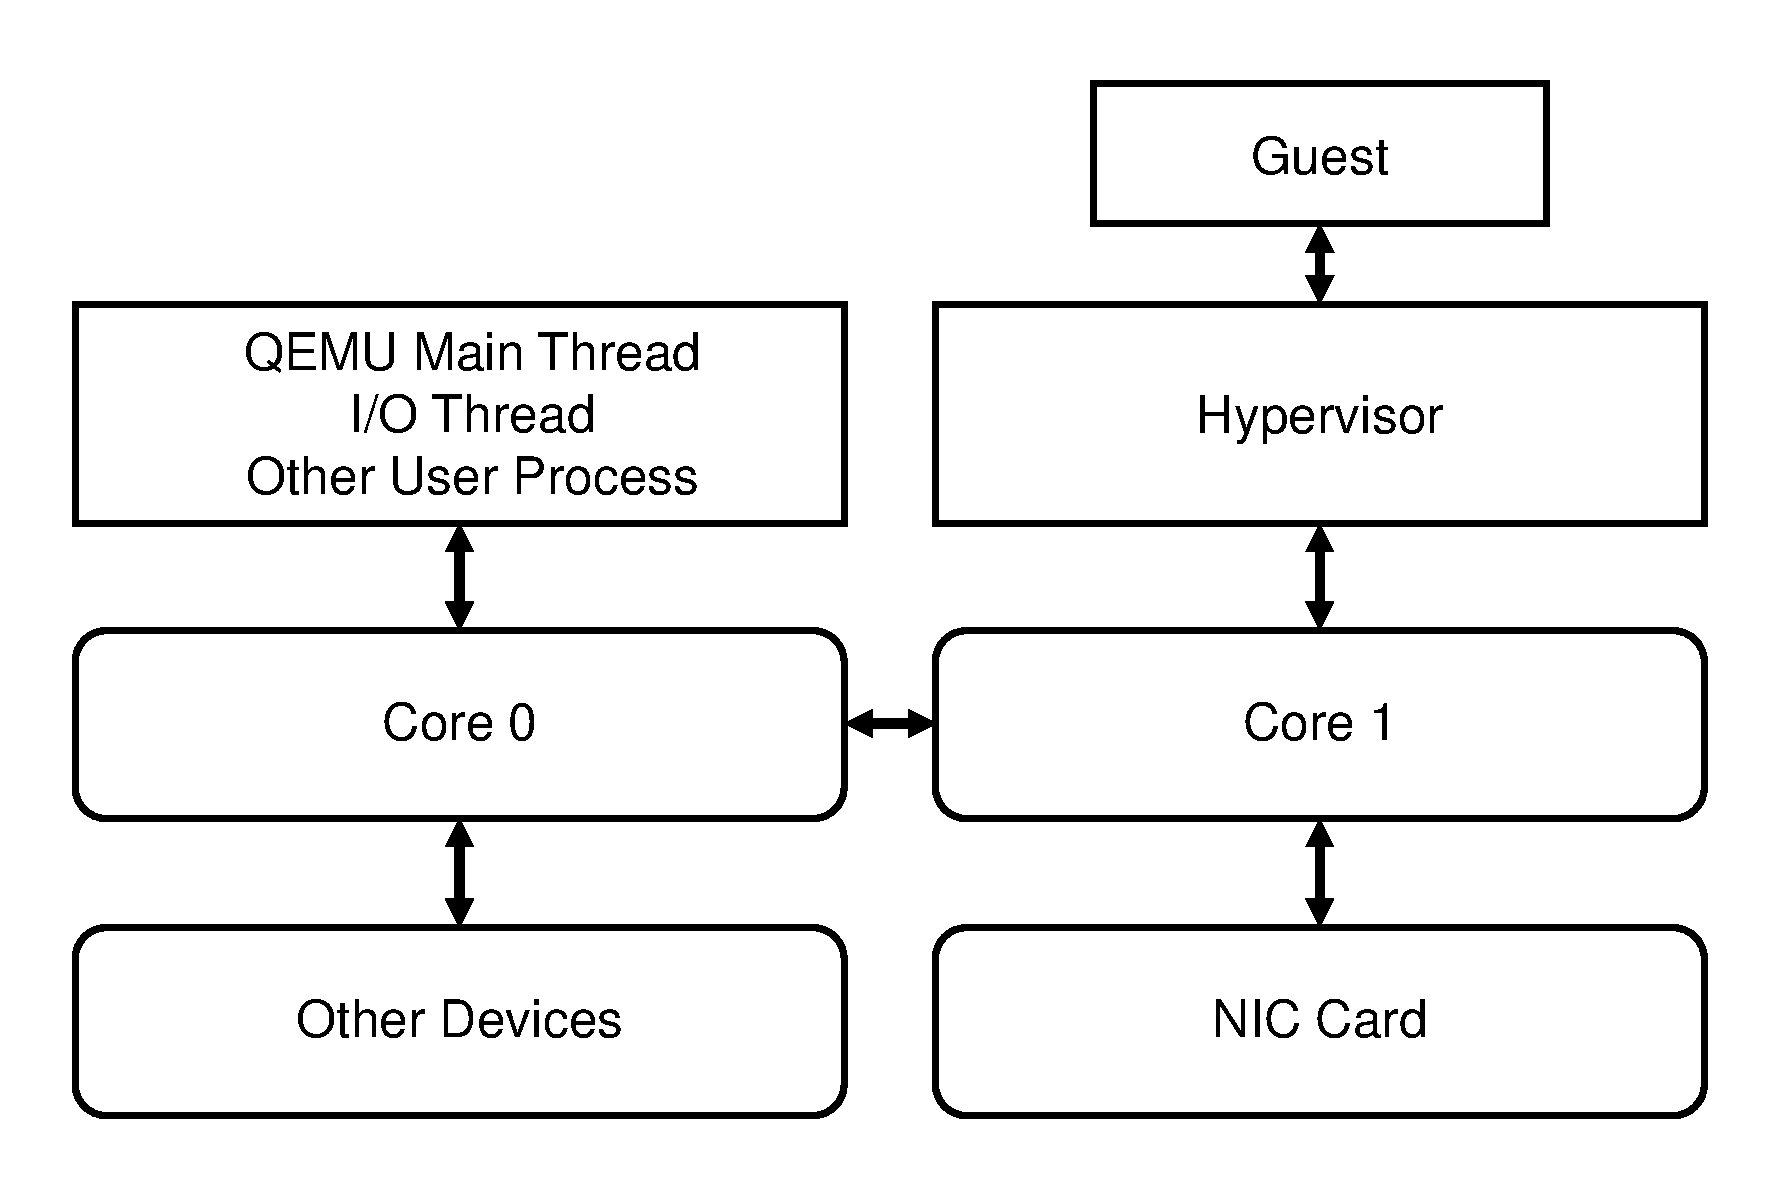
\includegraphics[width=0.4\textwidth]{figures/nested_virtualization_overhead_setup.pdf}
%  \caption{Optimizations to reduce overhead of nested virtualization: dedicated and isolated CPUs with Posted Interrupt support and halt\_poll\_ns disabled.}
%  \label{fig:optimizations}
  %\includegraphics[width=15cm,height=6cm,keepaspectratio]{architecture__1_.jpg}
%\end{figure}

\subsubsection{Mitigating Nesting Overheads}
\label{sec:overhead}
In comparison with the traditional single-level virtualization 
setup, where the hypervisor directly controls the hardware,
nested virtualization can introduce additional emulation overheads, especially for I/O virtualization. To mitigate such overhead, \arch uses the direct device assignment of network interface cards (NIC) to the hypervisor. 

%\textbf{Background}
Existing virtualization techniques (e.g., KVM \cite{kivity2007kvm}) support the full virtualization mode through device emulation \cite{sugerman2001virtualizing} and para-virtualization using virtio drivers \cite{russell2008virtio, barham2003xen}  in VMs. 
%They also support direct device assignment  to the guest \cite{ben2006utilizing}. 
For example, QEMU \cite{bellard2005qemu} emulates I/O devices requiring no modifications to VMs. When VMs access the devices, the I/O instructions are trapped into hypervisor leading to a number of VM/host context switches, resulting in lower performance of VMs. The para-virtualized devices offer better performance compared to device emulation, as the modified drivers in VMs avoid excessive VM/host switches for the I/O workloads. With Intel's VT-d \cite{abramson2006intel}, direct device assignment offers improved performance, as VMs directly interact with the devices bypassing the hypervisor.    
%With hardware virtualization technology, 
Further, SR-IOV \cite{dong2008sr} enables a single network device to present itself as multiple virtual NICs to VMs through virtual functions (VFs). Using a VF, a VM directly interacts with the network device --- with Intel's hardware support, VMs can directly access device memory through IOMMU which converts VMs physical addresses to host physical addresses.

%\textbf{Direct Device Assignment of Network Interface Card}
In this paper, \arch uses VFs to achieve network performance in nested guest to match the performance of a single-level guest and minimize the CPU Utilization in hyperplexor. VFIO \cite{vfiodriver} driver supports direct device assignment to a virtual machine. As shown in \fref{fig:vFresharch} every hypervisor running on hyperplexor is assigned one virtual function. The guest running on hypervisor uses para-virtualized driver to run the I/O workloads. \arch further applies many optimizations to provide hypervisor with enough resources and reduce the CPU utilization on hyperplexor. The goal is to run the hypervisor with minimum hyperplexor intervention. We describe the optimization techniques in detail in the following sections.

\begin{figure}[t!]
 	  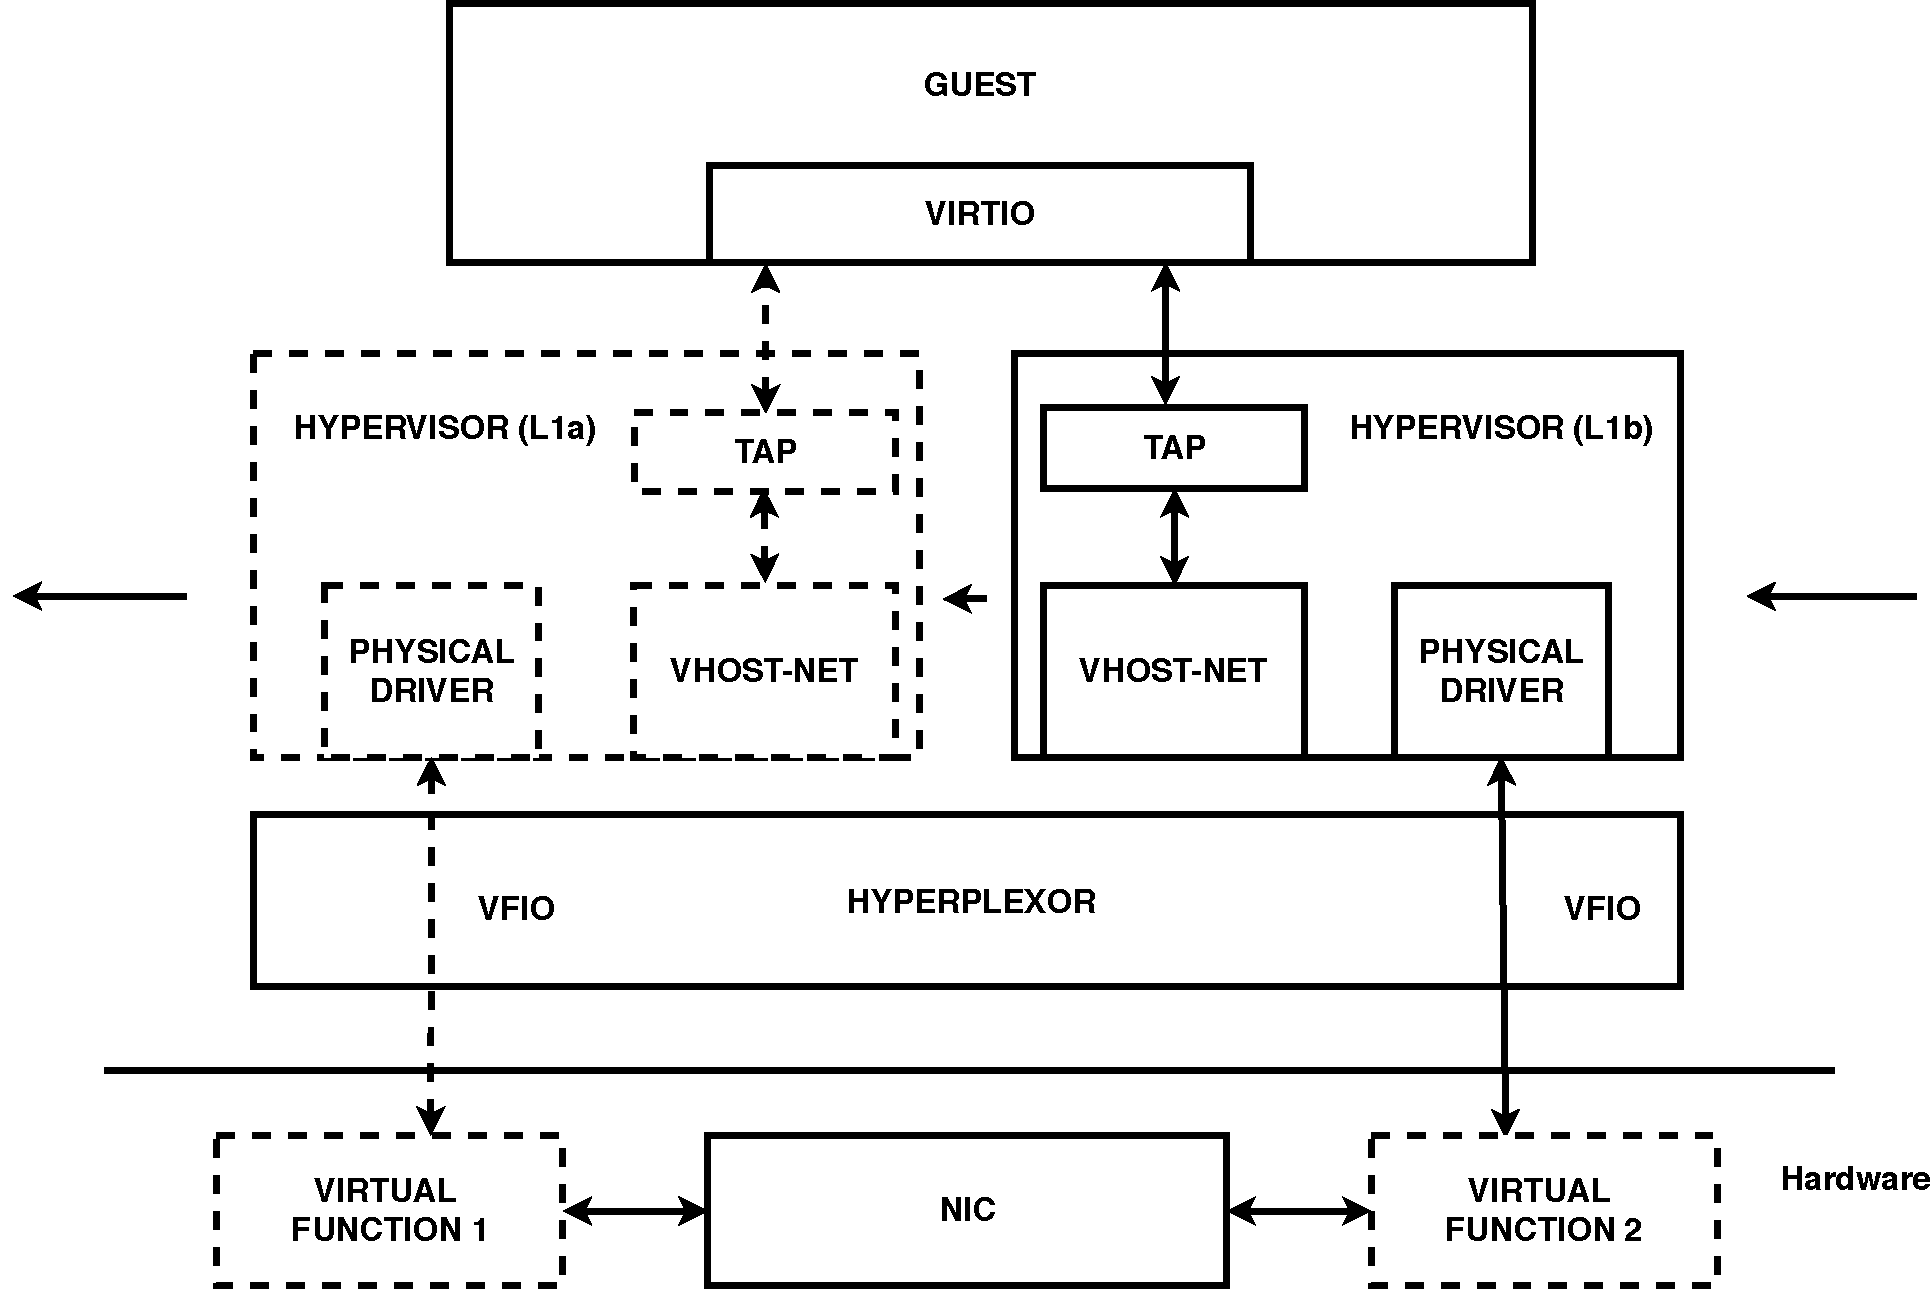
\includegraphics[width=0.45\textwidth]{figures/architecture_modified.pdf}
  \caption{Architecture for hypervisor replacement with direct-device assignment and thin hyperplexor.}
%TODO: Please fix this caption
  \label{fig:vFresharch}
  \vspace{0.2in}
  %\includegraphics[width=15cm,height=6cm,keepaspectratio]{architecture__1_.jpg}
\end{figure}

%\begin{itemize}
%\item \textbf{\textit{Reducing Memory Footprint of Hyperplexor}}
\para{Memory Footprint:}
As the hyperplexor involvement is minimal, it is configured with essential packages, device drivers and services reducing the memory consumption. The size of the hyperplexor without VM is 90 MB of the available memory compared to the Ubuntu server size 154 MB. The userspace processes and services that where not necessary to run the L1 hypervisor with direct-device assignment were identified and removed. The Linux kernel 4.13.0 is compiled with 32 kernel modules compared to 120 kernel modules in Ubuntu server. 
    
%	\item \textbf{\textit{HLT Exits}}
%halt_poll_ns is a kvm kernel module parameter. When guest VCPU has no work to do or goes idle, the VCPU goes to sleep by executing HLT instruction which causes a VM Exit. The parameter halt_poll_ns specifies how much time the VCPU needs to poll before executing the HLT instructions. This polling interval helps in making the guest more responsive for workloads like the network.

\para{HLT Exits:}
Although a directly assigned network device to a VM gives better performance, the CPU utilization on the host is high due to the idle polling of VCPUs. When the VM is idle, QEMU halts the idle VCPUs by executing a HLT instruction which triggers a VM exit. When the work is available for the VCPU, it has to be woken up to execute the new work. This transition from idle to ready state is costly as it involves context switch and hinders the performance of the VM. To avoid too many transitions, before executing the HLT instruction the VCPU polls for the specified amount of time to check if there is any additional work to be executed. This idle polling of VCPUs reduces the number of VM exits but increases CPU utilization on host. To reduce CPU utilization on host, we disable polling of VCPUs before executing HLT instruction. 
KVM provides a \texttt{halt\_poll\_ns} kernel module parameter to set the value of \texttt{halt\_poll\_ns}. To disable polling we set \texttt{halt\_poll\_ns} to zero. In this paper, as we assign the network device to the hypervisor, we disable the halt polling of hypervisor VCPUs to reduce the CPU Utilization in hyperplexor.
    
   %\item \textbf{\textit{Posted Interrupts}}
\para{Posted Interrupts:}
     When an external interrupt arrives, the CPU switches from non-root mode to root mode (VM Exit) and transfers the control to the hypervisor. Increase in number of external interrupts causes increase in VM Exits. With Intel's VT-d posted interrupt support the external interrupts are delivered to guest without hypervisor intervention. With posted interrupts support the hypervisor can inject a virtual interrupt to guest by updating the fields in the VMCS in guest or non-root mode. Hypervisor notifies the arrival of posted interrupt to the guest by setting the fields Posted Interrupt Request (PIR), Notification Vector (NV) and Outstanding Notification (ON) in Posted Interrupt Descriptor structure. The PIR field is 256 bit long and provides storage for posting the interrupts. The NV field is used to notify the interrupt vector to the guest. The ON bit indicates the processing status of the posted interrupt. We enable posted interrupt feature on the hyperplexor and deliver external interrupts directly to hypervisor without causing exits to hyperplexor.  
     
%\item \textbf{\textit{Dedicated Cores}}
\para{Dedicated Cores:}
All the system processes are running on two cores except the VCPUs which run on dedicated cores. The remaining CPUs are isolated and each VCPU is pinned to one CPU to avoid other processes from contending with VCPUs. 
%As shown in Figure~\ref{fig:optimizations}. 
The QEMU process along with other hyperplexor processes are pinned to CPU0 \& CPU1, and the hypervisor VCPUs run on the dedicated cores. 

%------OLD Stuff----------------------------------------
% \begin{table*}[!htb]
%\small
%  \begin{tabular}{|c|l|l|l|}
%   \hline
%  \arch API & \multicolumn{1}{c|}{Input Parameters} & \multicolumn{1}{c|}{Return Value} & \multicolumn{1}{c|}{Description}\\
%  \hline
%  \hline
%  hypercall\_set &unsigned long base\_addr\_of\_l2gfn\_list, &0 on success,  & Given the VM on the stale hypervisor, \\ 
%  &unsigned long base\_addr\_of\_l1gfn\_list, &failure code otherwise & pass a list of L2-to-L1 page mappings to hyperplexor  \\
%  &unsigned int count, & & for setting up \arch table entries  \\
%  &unsigned int vmid & & storing the L2-to-PA page mappings\\
%  \hline
%
%  hypercall\_map &unsigned long base\_addr\_of\_l2gfn\_list, &0 on success, & Given the VM on the replacement hypervisor, \\
%  &unsigned long base\_addr\_of\_l1gfn\_list, &failure code otherwise & pass a list of L2-to-L1 page mappings to hyperplexor \\
%  &unsigned int count, & & to look up \arch table  \\
%  &unsigned int vmid && for creating L2-to-PA mappings\\
%  \hline
%  
%    hypercall\_set &unsigned long base\_addr\_of\_gva\_list, &0 on success,  & Given a process on the stale OS, \\ 
%  &unsigned long base\_addr\_of\_gfn\_list, &failure code otherwise & pass a list of process-to-VM page mappings   \\
%  &unsigned int count, & & to hypervisor for setting up \arch table entries  \\
%  &unsigned int pid & & storing the GVA-to-PA page mappings\\
%  \hline
%
%  hypercall\_map &unsigned long base\_addr\_of\_gva\_list, &0 on success, & Given the process on the replacement hypervisor, \\
%  &unsigned long base\_addr\_of\_gfn\_list, &failure code otherwise & pass a list of process-to-VM page mappings\\
%  &unsigned int count, & & to look up \arch table  \\
%  &unsigned int pid && to hypervisor for creating GVA-to-PA page mappings\\
%  \hline
%\end{tabular}
%\caption{\arch API}
%\vspace{-0.2in}
%\label{tab:api}
%\end{table*}

%In our approach, we leverage grant table mechanism to transfer the mappings of guest from current hypervisor to updated hypervisor. The current hypervisor requests the hyperplexor to create grant entries in grant table. The updated hypervisor then requests the hyperplexor to map the guest page frame to physical page frames. 

%\textbf{\textit{Background}}
%In Xen, Virtual Machine Monitor (VMM) runs at the highest privilege level which coordinates with host domain (Dom0) or host OS to maintain isolation between guest domains (DomU) or guest OS. Xen supports both full-virtualization and para-virtualization modes. Para-virtualization mode is more efficient with lower virtualization overhead. However, it comes with a trade-off of modifying the guest OS.

%In Xen, the devices are managed by native device drivers run in isolated driver domain (IDD). The network device is presented as a virtual network device to a guest OS. The guest OS runs the front-end driver which shares a device ring buffer with the back-end driver in IDD or Dom0. In para-virtualization mode, a grant table\cite{Pratt05xen3.0} is used as a communication channel between domains. Each domain has a grant table and it is used to share or transfer the memory mappings between the domains. A grant table data structure is shared between Xen and the domain. The grant table entries are indexed using an integer field called grant reference. The reference field indicates which grantee can share the pages with the granter. 

%To share the pages, the granting domain advertises the page to be shared with other domains. The granting domain shares the grant reference ID with the receiving domain. The receiving domain maps the page by updating it's grant table entry. After the receiving domain has finished the operation on the page, the granting domain revokes the access to the page. For page transfer mechanism, after the granting domain transfers the page to the receiving domain, the page is freed from the granting domain. Transferring the pages between the domains reduces the memory-copy overhead which increases with increase in data-size.   

%\subsubsection{Hypervisor Switching}
%In the proposed work, we use grant table to share and finally transfer the ownership of the physical page frames from old hypervisor to the current hypervisor. As shown in Figure~\ref{fig:mapping}, the grant table is maintained by the hyperplexor which is responsible to transfer the ownership of the guest memory. The grant table holds the list of all the guest page frame mappings to the memory page frames. It also contains a guest ID field which signifies the ownership of the guest page frames.

%During boot time, VM1 pre-allocates its memory by pinning the L2 pages in memory (i.e., the swap option is disabled). By doing this, the virtual EPT for VM1 in its L1 hypervisor and the shadow EPT in the L0 hyperplexor get populated, resulting in no further virtual EPT or shadow EPT faults during the runtime. The \arch table is created when VM1 requests the L1 hypervisor to pin all the L2 pages --- the L1 hypervisor invokes a series of \texttt{hypercall\_set} hypercalls each with a list of L2-to-L1 page mappings (i.e., from the virtual EPT), and the hyperplexor uses received mappings to populate the \arch table for VM1 as stated above.

%and for the guest in the hyperplexor during the boot time.  As the guest memory pages are pinned in memory and the swap option is turned off the memory mappings of the guesteare not bound to change.


%The replacement hypervisor prepares a new VM, VM2, in the {\em replacement} state (i.e., not running). VM2 is allocated with the same range of L2 pages as VM1, and then requests the replacement hypervisor to map its L2 pages to the same physical pages as VM1.
%After populating the L2-to-L1 page mappings, the replacement hypervisor invokes a series of \texttt{hypercall\_map} hypercalls each with a list of L2-to-L1 page mappings to the hyperplexor. The hyperplexor installs the L1-to-PA page mappings in the replacement hypervisor's EPT table using the \arch table, as stated above. 

%At this stage, VM2 still stays in the replacement state (i.e., not running) and hence does not corrupt the memory of VM1. VM2 waits for the VCPU and I/O device state of VM1 before starting running. VM1 on the stale hypervisor is then paused and the VCPU and I/O device state are transferred to VM2 on the replacement hypervisor.  Once VM1 is paused, the VM ID of the \arch table is changed to the VM2's ID. 



%As shown in Figure~\ref{fig:mapping} when the updated hypervisor has to replace the current hypervisor, the guest QEMU that runs on updated hypervisor before the migration requests updated hypervisor to map it's guest page frames to the physical page frames in advance using the grant table. The hyperplexor maps the new guest page frames to physical page frames using grant table. At this stage, the QEMU on updated hypervisor is in migrate state and does not corrupt the memory as it does not contain the current vCPUs and I/O device information. This maintains the consistency in memory. As a result the ownership of the physical page frames in grant table is not yet transferred to the new guest.    

 

\section{\arch for OS Replacement}
Using containers to host applications becomes a common usage scenario 
in today's cloud~\cite{aws, gcpkubernetes, azureks, ibmkubernetes, vmwarepks}. 
Under this scenario, the act of OS replacement can be viewed as 
moving the state of all containers from the old VM with the 
stale OS to a new VM with the replacement OS. Again, we leverage 
intra-host live migration to avoid inter-host communication.

\subsection{Memory Translation for Containers}
The memory management for containers belongs to the above-mentioned single-level virtualization. As shown in \fref{fig:mappingc}, the page table of a process (belonging to a container) running in the VM stores the mappings between the guest virtual addresses (GVA) of the process and the guest physical addresses (GPA) of the VM. The hypervisor uses the EPT to map GPA to physical addresses (PA). 

\subsection{OS Replacement Overview}
To replace the stale OS for a container, the hypervisor creates a new VM with the replacement OS, and transfers the ownership of all the container's pages to this new VM.

\arch transfers the memory ownership using the \arch table, whose purpose is similar to that described for hypervisor replacement.
The  per-process \arch table stores the memory mappings from the pages of the container to the  pages of the physical memory, constructed by the stale OS, and is leveraged by the new OS for reconstructing the 
memory address space of the container during OS replacement. 

The replacement process on the new VM first reconstructs all the GVAs of the container. The VM kernel then allocates corresponding GPAs and sets up the GVA-to-GPA page mappings in the page table of the container. Finally, the new VM's kernel invokes a series of \texttt{hypercall\_map} hypercalls to the hypervisor, which installs the GPA-to-PA page mappings in the new VM's EPT table using the \arch table.

The transfer of execution control is performed as follows:
The container's execution is paused at the stale OS
and its execution state (all state of the container) 
are transferred to the replacement VM's control, which then resumes execution of the new VM. Finally, once the control of the container is transferred to the replacement OS, 
the stale OS can unmap the container's memory from its address space and be safely deprovisioned. 

\begin{figure}[t!]
 	  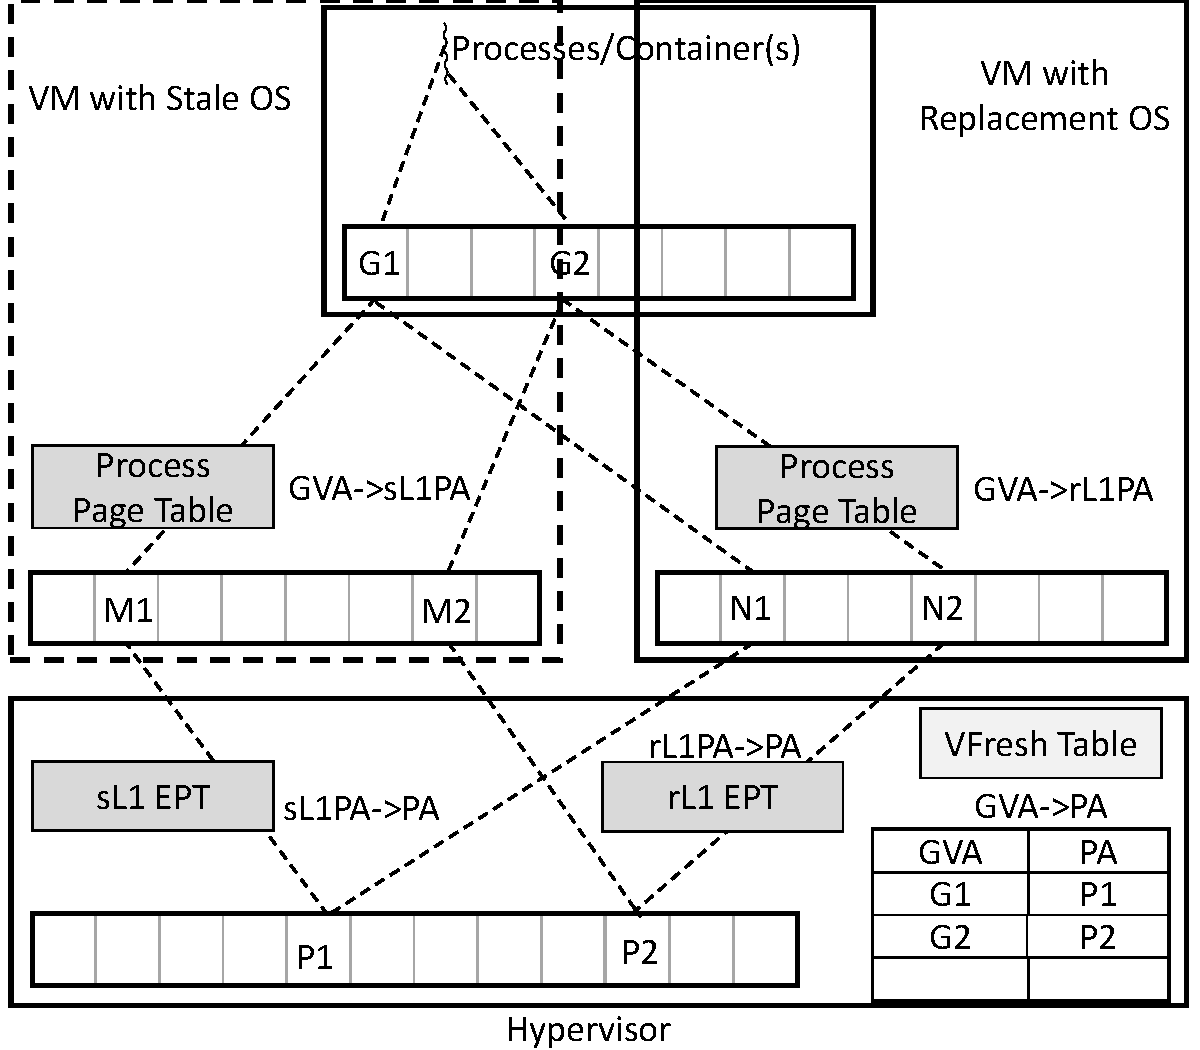
\includegraphics[width=0.45\textwidth]{figures/vfresh-table-container.pdf}
  \caption{Memory translations for OS replacement.}
  \label{fig:mappingc}
  %\includegraphics[width=15cm,height=6cm,keepaspectratio]{architecture__1_.jpg}
  \vspace{0.2in}
\end{figure}


%Essentially, a container consists of a hierarchy of processes as well as isolation mechanisms (e.g., \texttt{cgroups} and \texttt{namespaces} in Linux). If not specified, processes running upon an OS belong to a default container. Hence, moving a container from one VM to another for OS replacement needs to copy the state of all processes in the container from one VM to another. Again, \arch's OS replacement relocates the memory ownership of all processes instead of copying memory data. The design of \arch's OS replacement is  similar to the above hypervisor replacement, and we focus on the differences in the OS replacement.




    
%\subsection{OS Switching}
%During OS replacement, the stale VM's kernel provides the GVA-to-GPA page mappings for \texttt{hypercall\_put} hypercalls to build an \arch table. Such mappings can be obtained by walking through the page table of the process in the stale VM's kernel. These mappings can also be obtained using a user-level replacement tool (e.g., CRIU~\cite{criu}), which dump and transfer memory state from the user space (e.g., reading from \texttt{$\slash$proc$\slash$[PID]$\slash$pagemap}). To support such a user-level live OS replacement implementation, \arch provides a new system call, \texttt{syscall\_set}, which takes a list of GVA-to-GPA mappings from the user space. Thus, in this syscall, the VM kernel simply passes received GVA-to-GPA mappings to the hypervisor via \texttt{hypercall\_put} hypercalls.  

%The replacement process on the new VM with the replacement OS first reconstructs all the GVAs (e.g., with the \texttt{mmap} system call). The VM kernel then allocates corresponding GPAs and sets up the GVA-to-GPA page mappings in the page table of the process (e.g., with the \texttt{set\_pte\_at} system call). Finally, the new VM's kernel invokes a series of \texttt{hypercall\_map} hypercalls to the hypervisor, which installs the GPA-to-PA page mappings in the new VM's EPT table using the \arch table as stated above. 

%To further support user-level live OS replacement implementations, which dump and transfer memory state from the user space (e.g., CRIU \cite{criu}), \arch provides a  system call, \texttt{syscall\_set}. Similar to \texttt{hypercall\_set}, \texttt{syscall\_set} takes a list of GVA-to-GPA mappings from the user space. Differently, the user-level replacement tool should prepare these mappings (e.g., reading from \texttt{$\slash$proc$\slash$[PID]$\slash$pagemap}). Thus, in this syscall, the VM kernel simply passes received GVA-to-GPA mappings to the hypervisor via \texttt{hypercall\_set} hypercalls.  

%Using a memory copying based approach, reconstructing address space of the process on the VM with the replacement OS involves two steps: (1) creating the same GVAs (e.g., via \texttt{mmap}) as that of the process on the stale VM (from received memory mapping metadata); and (2) loading memory page contents (e.g., via \texttt{preadv}) from the received memory data. With given GVAs, loading memory page contents will establish all the mappings in two page tables --- the GVA-to-GPA page table of the process and the GPA-to-PA EPT of the VM with the replacement OS.


%\label{sec:destdesign}
%This syscall also needs to change the virtual address of the array passed from the user space to a set of disjoint GPAs before calling hypercalls). 
%\end{itemize}

%\begin{figure}[t!]
%  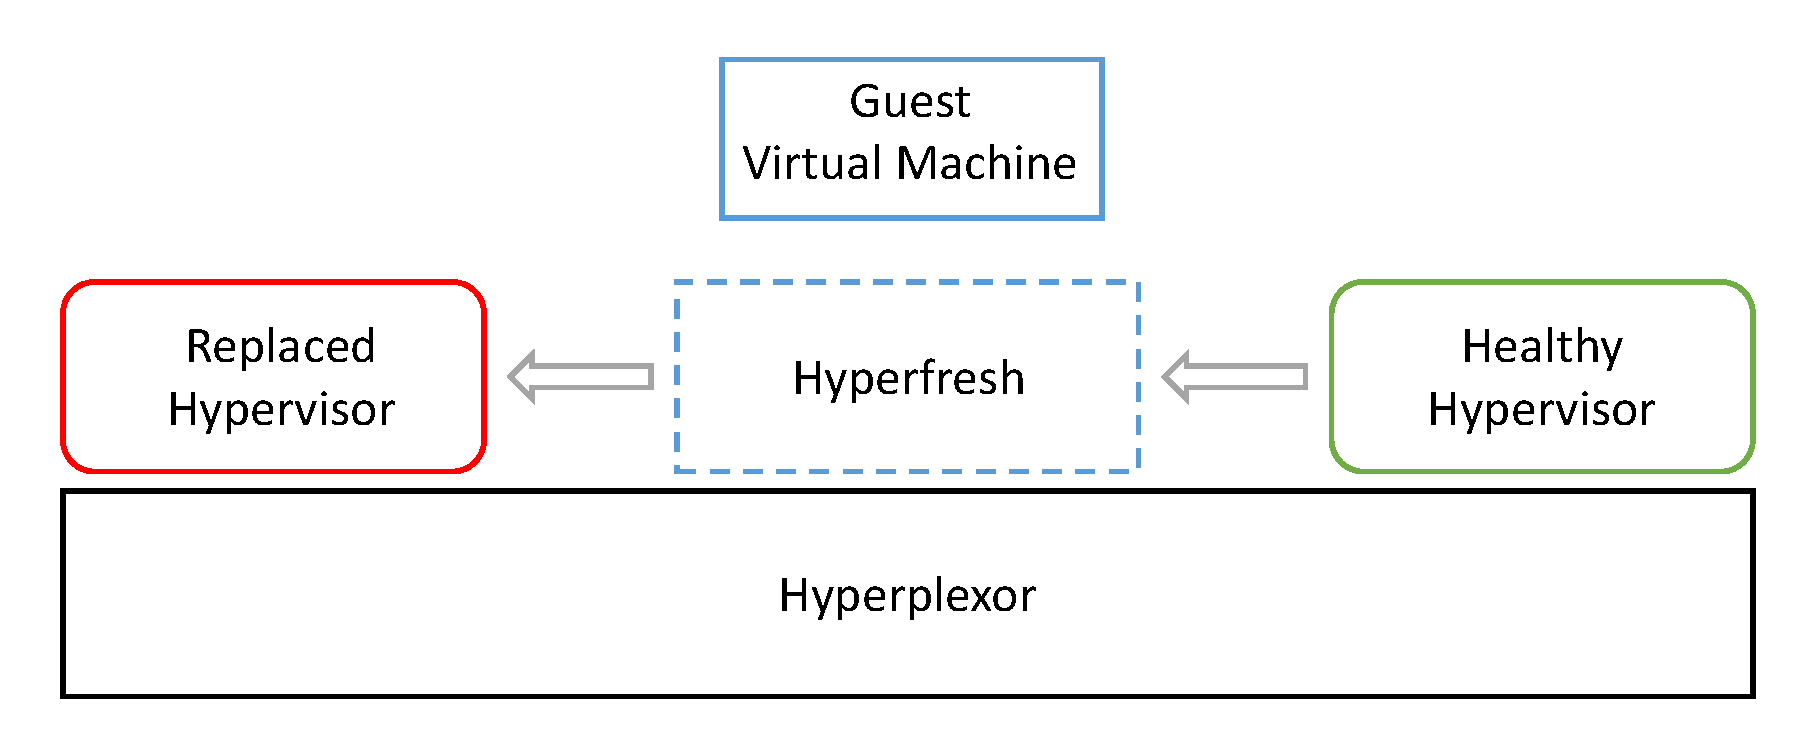
\includegraphics[width=0.5\textwidth]{figures/shift.pdf}
%  \caption{Hypervisor switching operation}
%  \label{fig:switching}
  %\includegraphics[width=15cm,height=6cm,keepaspectratio]{architecture__1_.jpg}
%\end{figure}

%\subsection{Hypervisor Switching}
%The guest initially runs on the hypervisor which in turn runs on thin hyperplexor. The guest pre-allocates it's memory by pinning the pages in memory during boot time. When the current hypervisor requires updates, a new hypervisor with pre-installed updates boots up  and runs the guest in migration state. The guest in migration state maps it's memory in advance to the guest running on current hypervisor using grant table mechanism described above and waits for the VCPU and I/O device state. The guest on current hypervisor is then paused and the VCPU and I/O device state are transferred to the guest on updated hypervisor as shown.

\subsection{Implementation Details}
We have implemented an OS replacement prototype based on CRIU \cite{criu} --- a well-known checkpoint/restore tool implemented in the user space. CRIU consists of two stages: checkpointing (on the source VM) and restoration (on the destination VM). By automating these two parts, we implemented the live OS replacement for containers. \arch's OS replacement operation involves the transfer of all the state of containers and their processes (e.g., file descriptors, memory maps, registers, namespaces, cgroups, etc.) except for memory content from the source VM (with the stale OS) to the destination VM (with the replacement OS).

In our implementation, when the OS replacement operation is invoked, one of the target processes in a container is paused. During the checkpointing phase, \arch collects all state of the process except for its memory content and build the \arch table. During the restoration phase, \arch restores the process state on the destination VM and relocates the memory ownership. In the final stage, \arch resumes running the process on the destination VM. The source VM unmaps the pages of the process from its address space. \arch repeats this process until all target processes are moved to the destination VM. Then the source VM can be gracefully shutdown. 

\para{The \arch Table.}
To build the \arch table for OS replacement, the hypervisor needs a list of GVA-to-GPA page mappings of a container from the stale OS. Similarly to the hypervisor replacement, \arch invokes multiple \texttt{hypercall\_put} hypercalls to pass a list of GVA-to-GPA page mappings to the hypervisor. For each received GVA-to-GPA page mapping, the hypervisor translates the page of GPA to the page of PA (i.e., using the VM's EPT), and puts the corresponding GVA-to-PA page mapping to the {\em \arch table}.

Restoring the address space of a container on the new VM needs to build GVAs, GPAs, and their mappings. Given the GVA-to-GPA page mappings of the container, the new VM's kernel invokes multiple \texttt{hypercall\_map} hypercalls to pass a list of GVA-to-GPA page mappings of the container to the hypervisor. 
For each received GVA-to-GPA page mapping, the hypervisor: (1) looks up the {\em \arch table} to find the GVA-to-PA page mapping with GVA as the key; and (2) installs the GPA-to-PA page mapping in the EPT page table of the new VM. 
%Similarly, the new VM's kernel can invoke multiple \texttt{hypercall\_map} hypercalls to pass all GVA-to-GPA mappings for fully relocating memory address space for the process on the new VM with the replacement OS.  

\para{Checkpointing.}
We modified CRIU's checkpointing code to replace the procedure of dumping memory content with the one which builds the \arch table by calling \arch's new system call, \texttt{syscall\_set}. The function takes an array of GVAs and the their mapped GPAs (e.g., reading from the \texttt{/proc/[PID]/pagemap} file).
%which stores the GVA-to-GPA mappings. 
We further use the \texttt{memalign} function to allocate page-size aligned memory for the input arrays. The \texttt{syscall\_set} system call translates the base address of the two arrays (containing GVAs and GPAs) into GPAs, and invokes the \texttt{hypercall\_set} hypercall to transfer the GPAs of the arrays to the hyperplexor.  
As stated above, the \texttt{hypercall\_set} hypercall obtains the GVA-to-PA mappings, and inserts them to the \arch table.

\para{Restoration.} On the destination VM, we modify CRIU's restoration code to replace the procedure of loading memory content with the one of transferring address space via \arch's new system call, \texttt{syscall\_map}. Before invoking  \texttt{syscall\_map}, the restorer needs to restore GVAs using the \texttt{mmap} system call. It then invokes \arch's \texttt{syscall\_map} to pass an array of GVAs. The \texttt{syscall\_map} system call in turn gets free VM memory pages, GPAs, and establish the GVA-to-GPA page mappings in the process's page table. With such GVA-to-GPA page mappings, the \texttt{syscall\_map} system call invokes the \texttt{hypercall\_map} hypercall to transfer these mappings to the hypervisor. As stated above, the \texttt{hypercall\_map} hypercall installs the GPA-to-PA page mappings in the destination VM's EPT table.


%\input{tex_files/overview.tex}
%\input{tex_files/tech_specs.tex}
%\input{tex_files/impl.tex}
%\input{Proposed_Framework.tex}
\section{Evaluation}
This section presents our comprehensive evaluation of the
benefits of \arch for hypervisor and OS replacement using both micro-benchmarks and real world applications.
\subsection{Hypervisor Replacement}
We run our experiments on server machines each with a 10-core Intel Xeon CPU of 2.2 GHz, 32 GB memory and one 40 Gbps Mellanox ConnectX-3 Pro network interface. All experimental results are averaged over five runs or more to increase the confidence in the results. 
%Table \ref{tab:setup1} shows the detailed setup configuration.

%Idle guest	Memory Variation			
%Guest Memory (GB)			1		2		3		4
%Inter-host					346.2	429		514		630.2
%Intrahost non-nested		224.4	285.2	347.6	409.4
%Intrahost nested (pv-pv)	509.2	695		963		1179
%Intrahost nested (pv-pt)	512.6	707		949.6	1173.6
%Hyperfresh					6.4		6.8		7		7.6

%The hypervisors are configured with 8GB and 4vCPUs.
%\begin{figure}[t!]
%  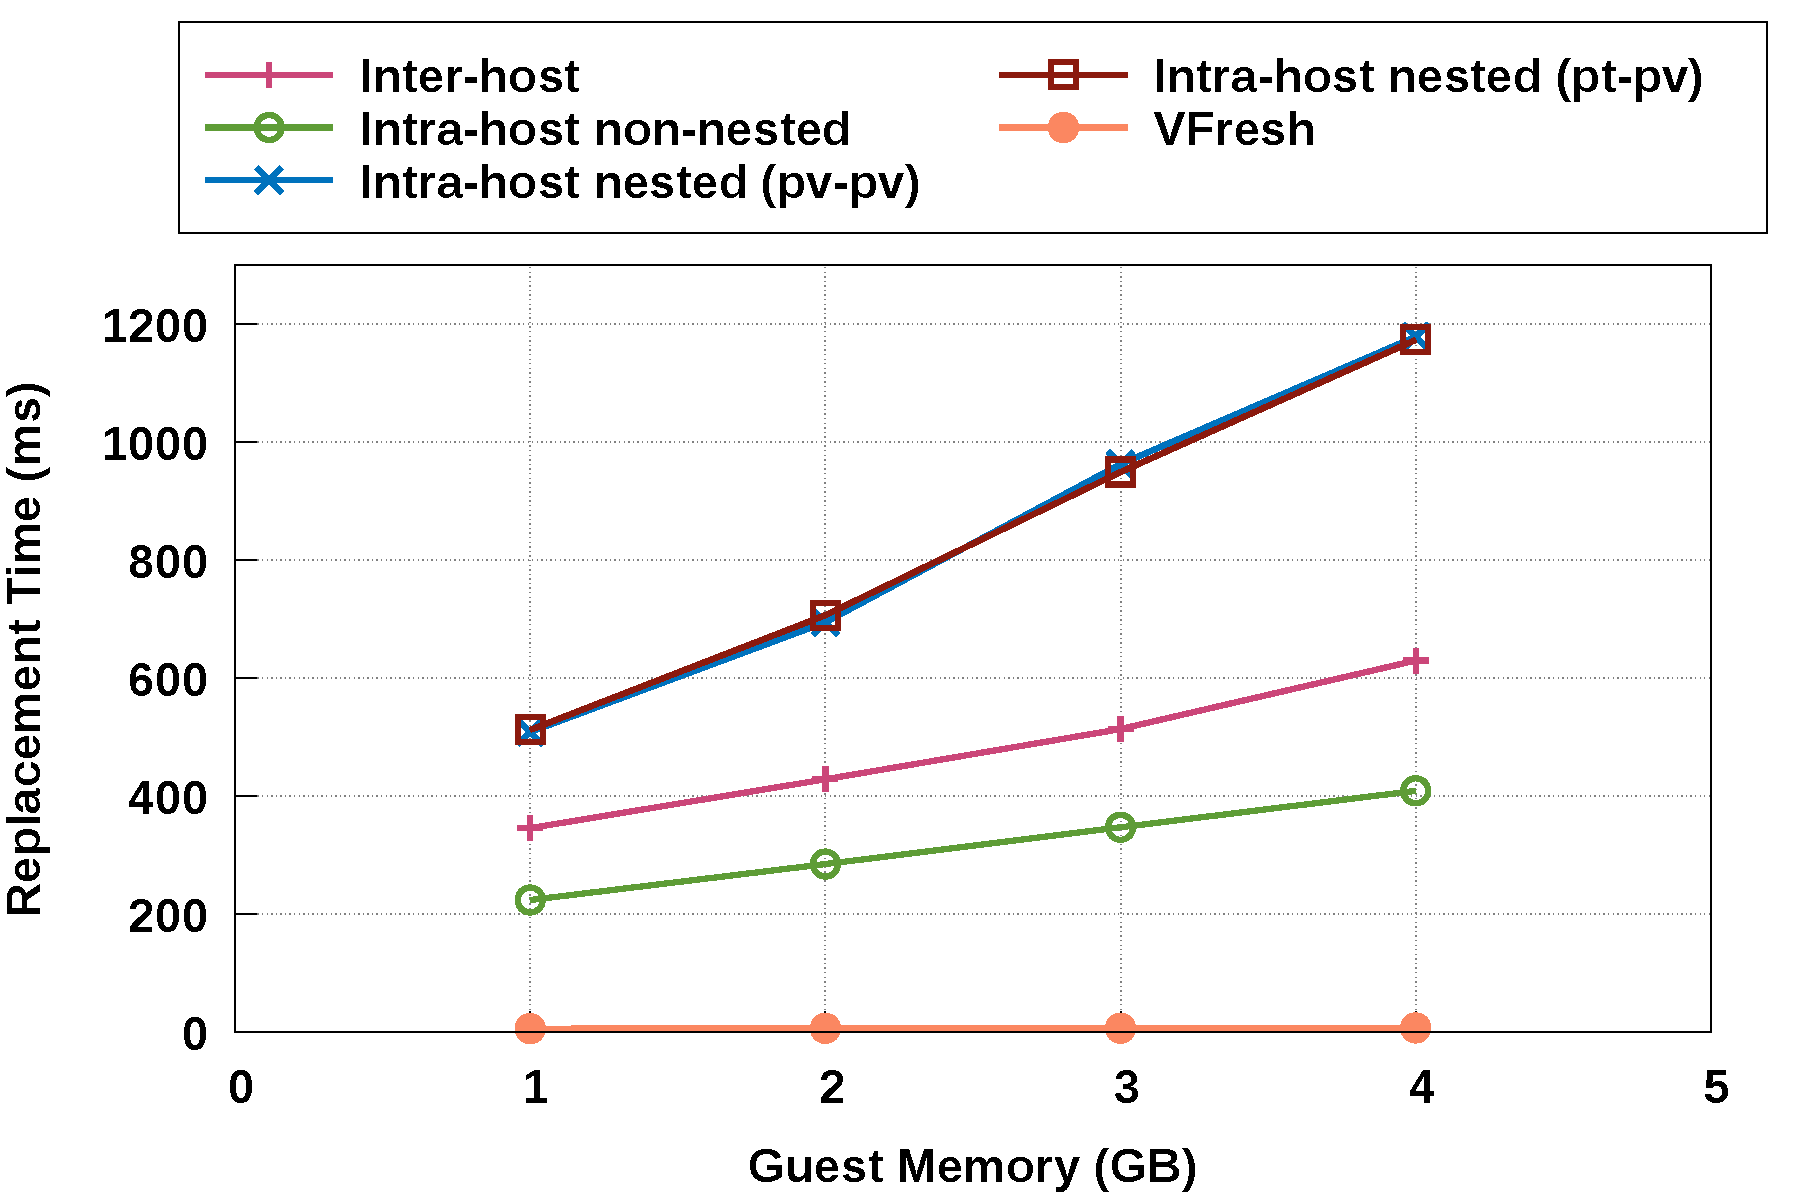
\includegraphics[width=0.45\textwidth]{figures/idle_guest_migration_with_vFresh.pdf}
%  \caption{Comparison of hypervisor replacement time for an idle guest with \arch and different setups.}
  %\caption{Comparison of refresh time for an idle guest - Our solution vs Optimized Pre-copy}
%  \label{fig:idleVfresh}
%  \includegraphics[width=15cm,height=6cm,keepaspectratio]{architecture__1_.jpg}
%\end{figure}

%\begin{figure}[t!]
%  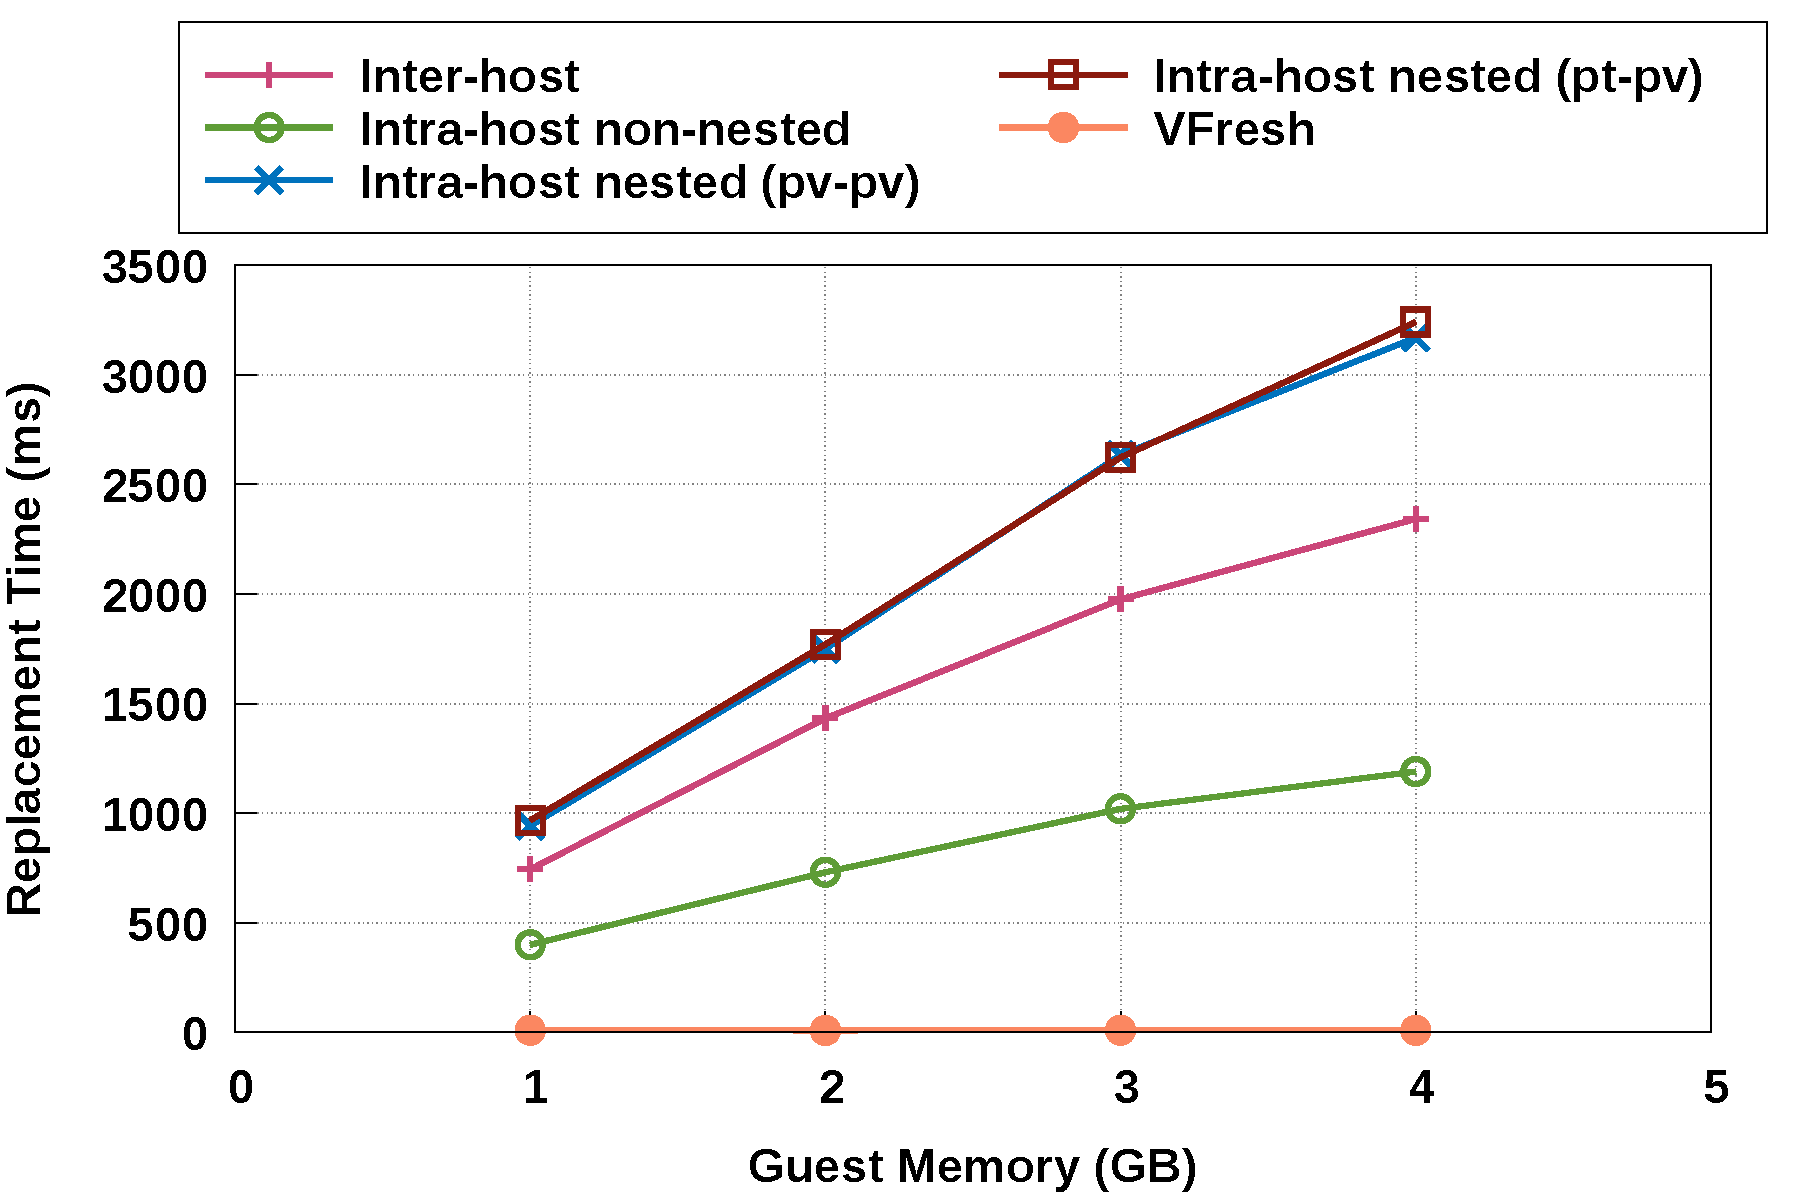
\includegraphics[width=0.45\textwidth]{figures/busy_guest_migration_with_vFresh.pdf}
%  \caption{Comparison of hypervisor replacement time for a guest performing write-intensive workloads with \arch and different setups.}
%  \label{fig:VfreshBusy}
%\end{figure}

%\begin{figure*}[t!]
% 	  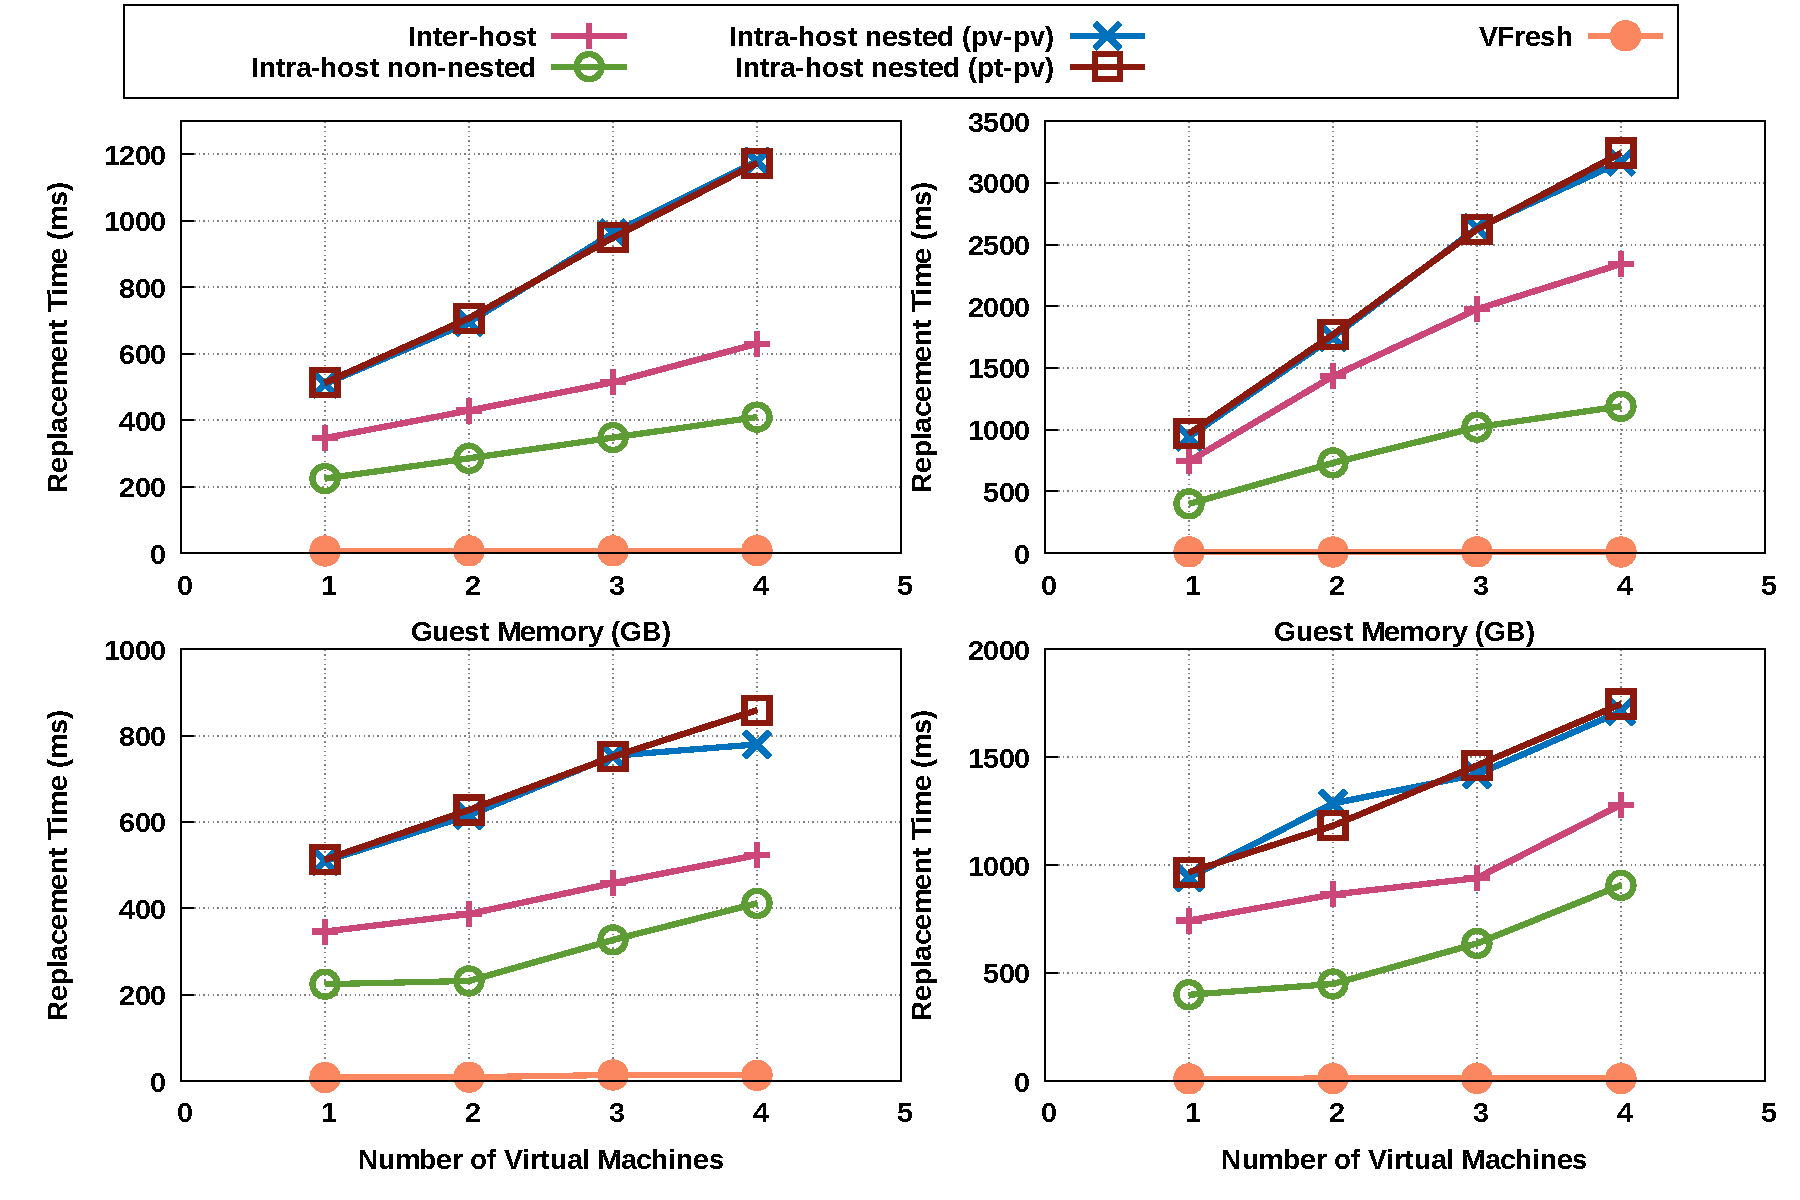
\includegraphics[width=0.98\textwidth]{figures/migration.pdf}
%  \caption{Architecture for hypervisor replacement with direct-device assignment and thin hyperplexor.}
%TODO: Please fix this caption
%  \label{fig:vFresharch}
  %\includegraphics[width=15cm,height=6cm,keepaspectratio]{architecture__1_.jpg}
%\end{figure*}

\begin{figure*}
\centering
\begin{minipage}{.43\textwidth}
  \centering
  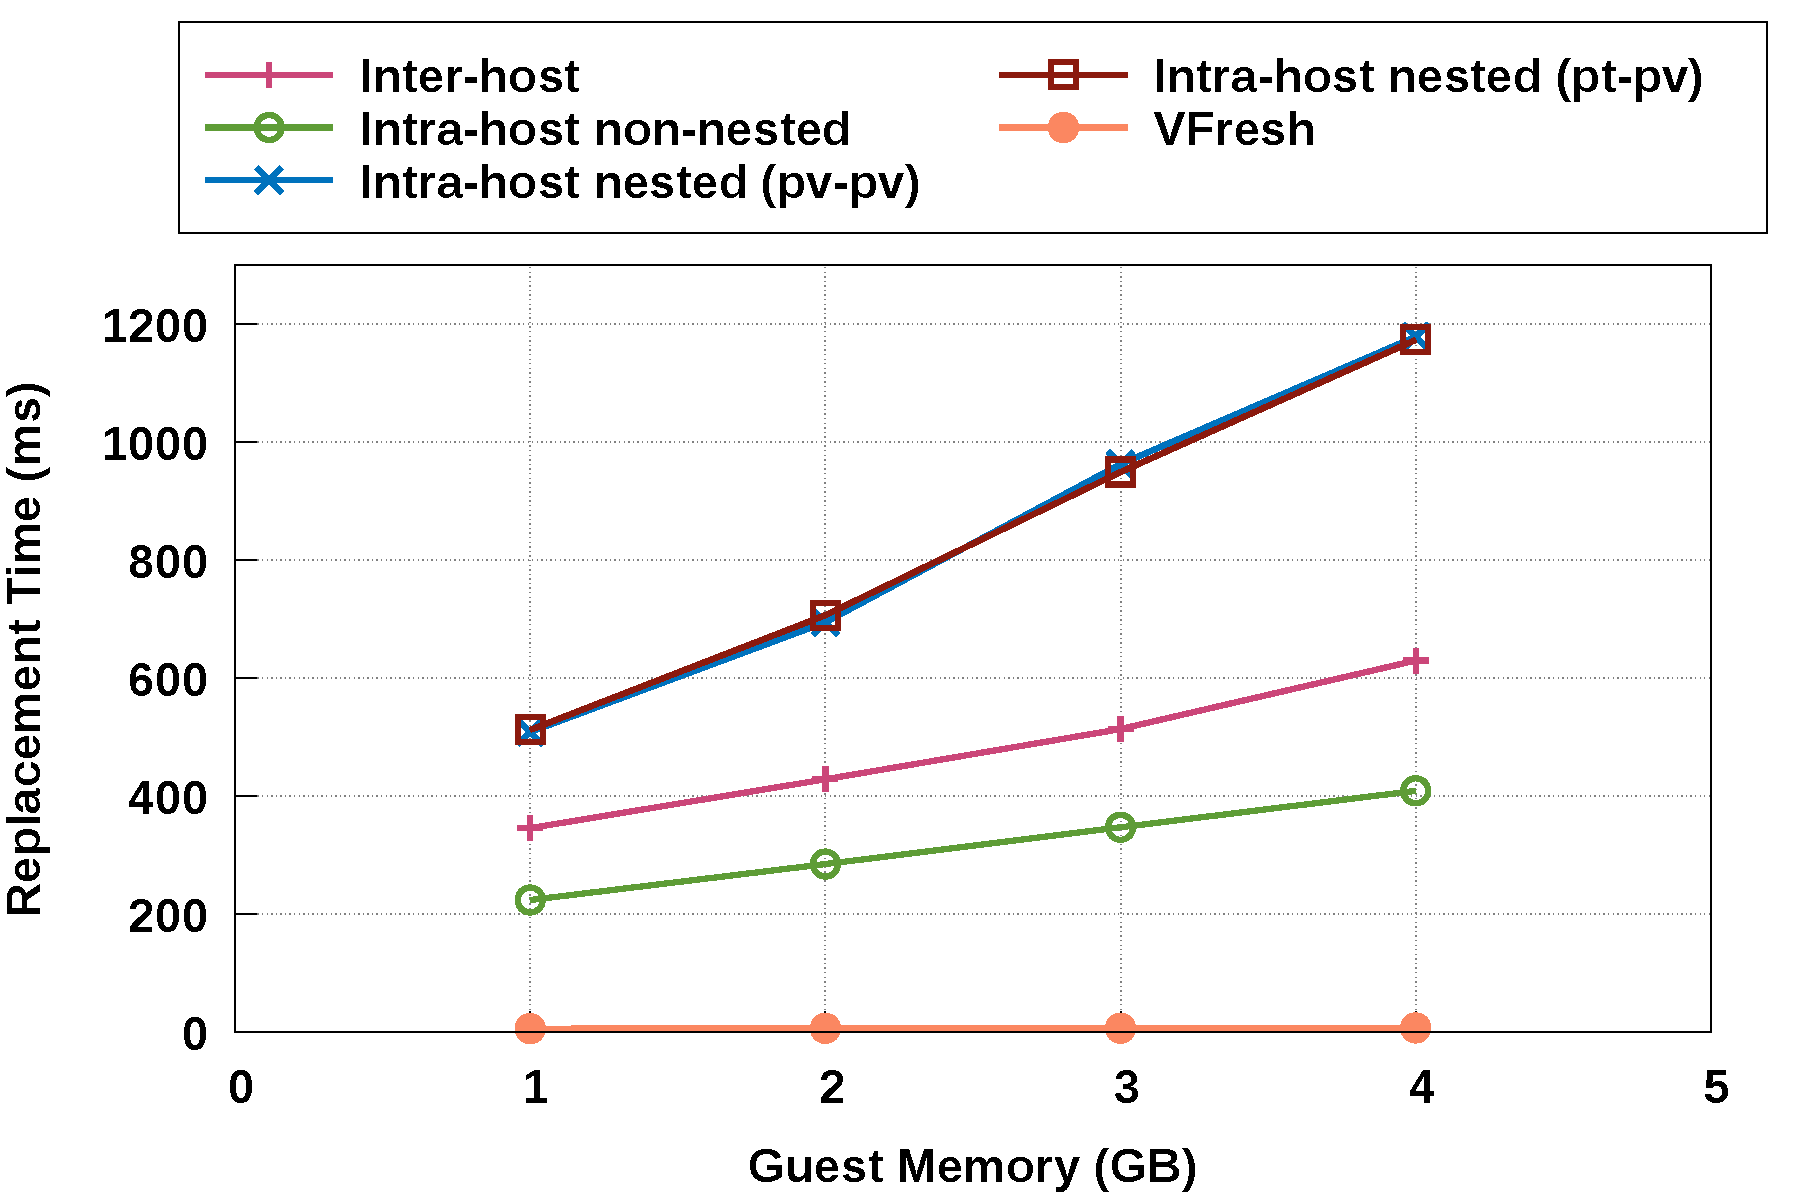
\includegraphics[width=.95\linewidth]{figures/idle_guest_migration_with_vFresh.pdf}
   \vspace{-0.1in}
  \captionof{figure}{Comparison of hypervisor replacement time for an idle VM with varying memory sizes.}
  \label{fig:idleVfresh}
\end{minipage}
\hspace{0.34in}
\begin{minipage}{.43\textwidth}
  \centering
  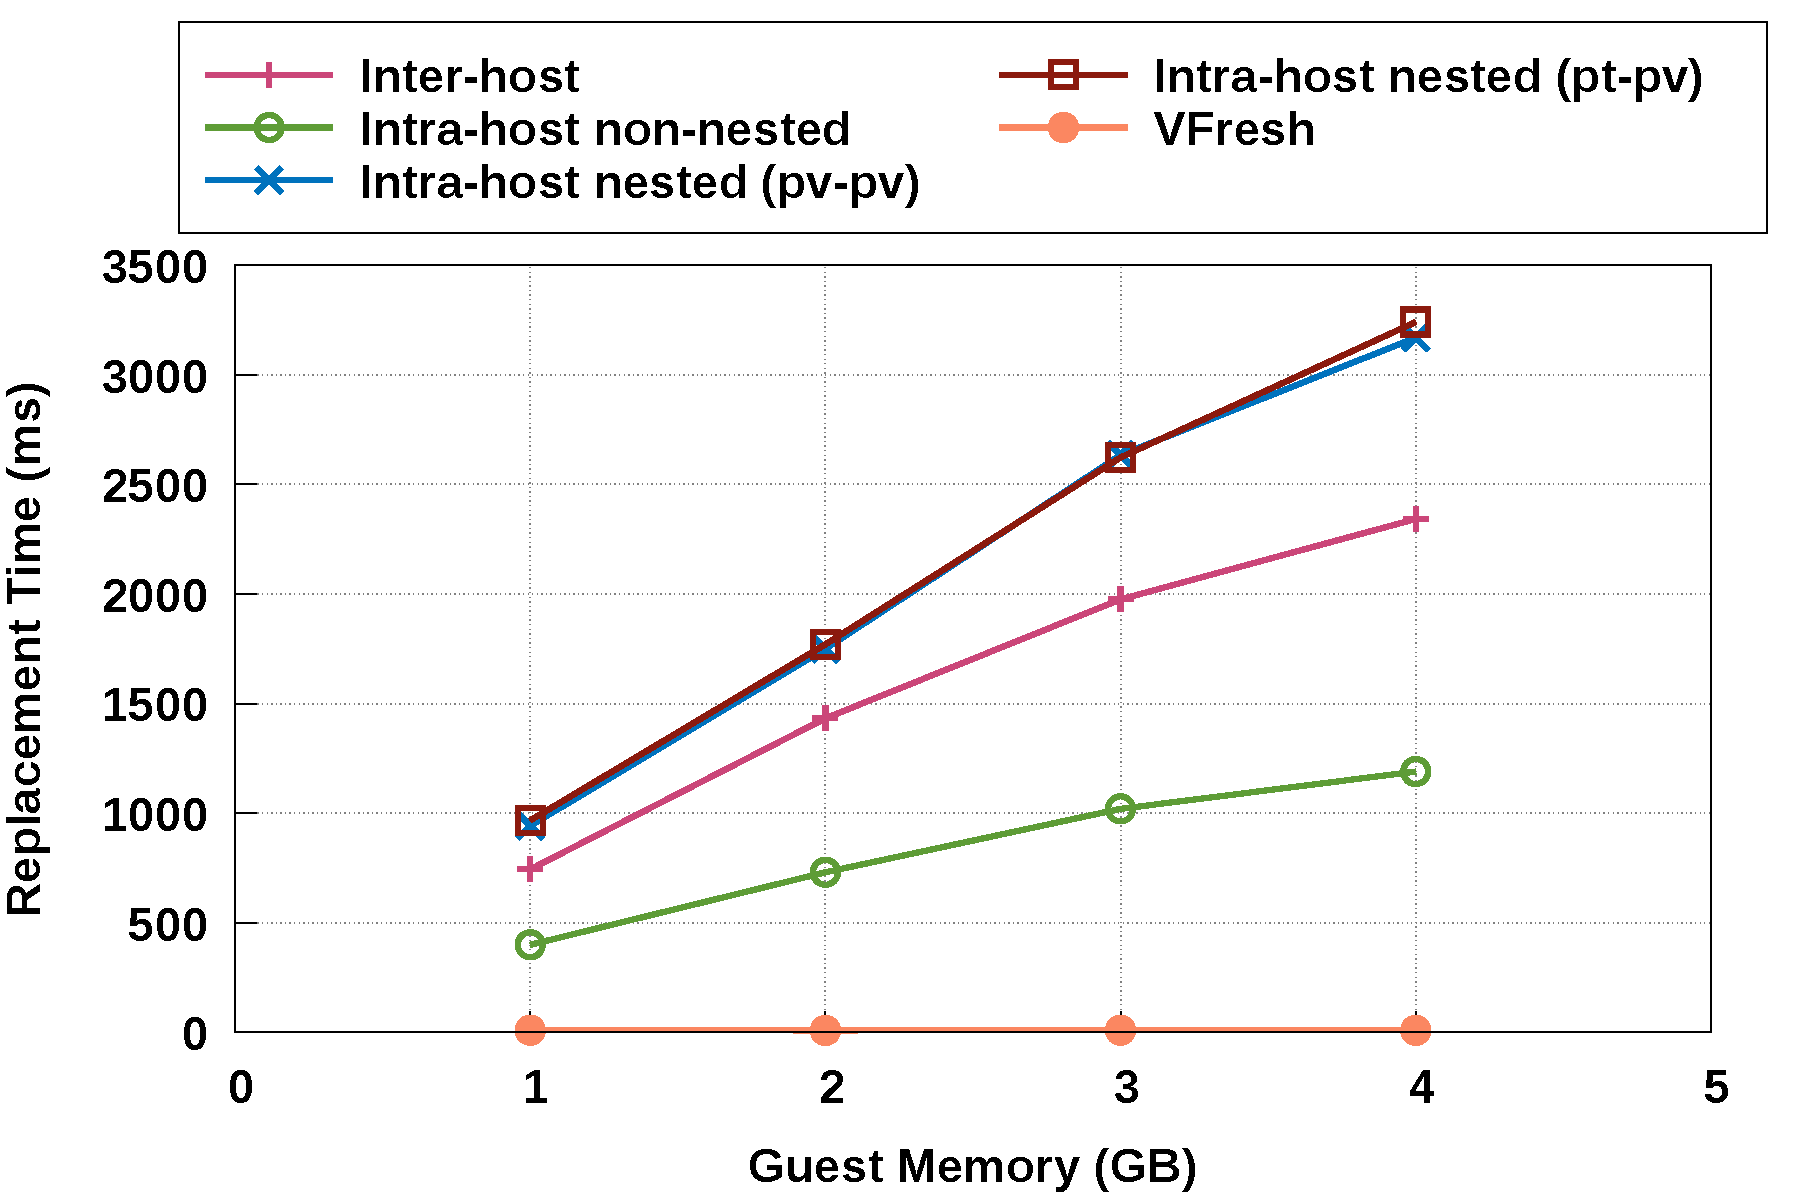
\includegraphics[width=.95\linewidth]{figures/busy_guest_migration_with_vFresh.pdf}
   \vspace{-0.1in}
  \captionof{figure}{Comparison of hypervisor replacement time for a write-intensive VM with varying memory sizes.}
  \label{fig:VfreshBusy}
\end{minipage}%
  \vspace{-0.1in}
\end{figure*}

\begin{figure*}
\centering
\begin{minipage}{.43\textwidth}
  \centering
  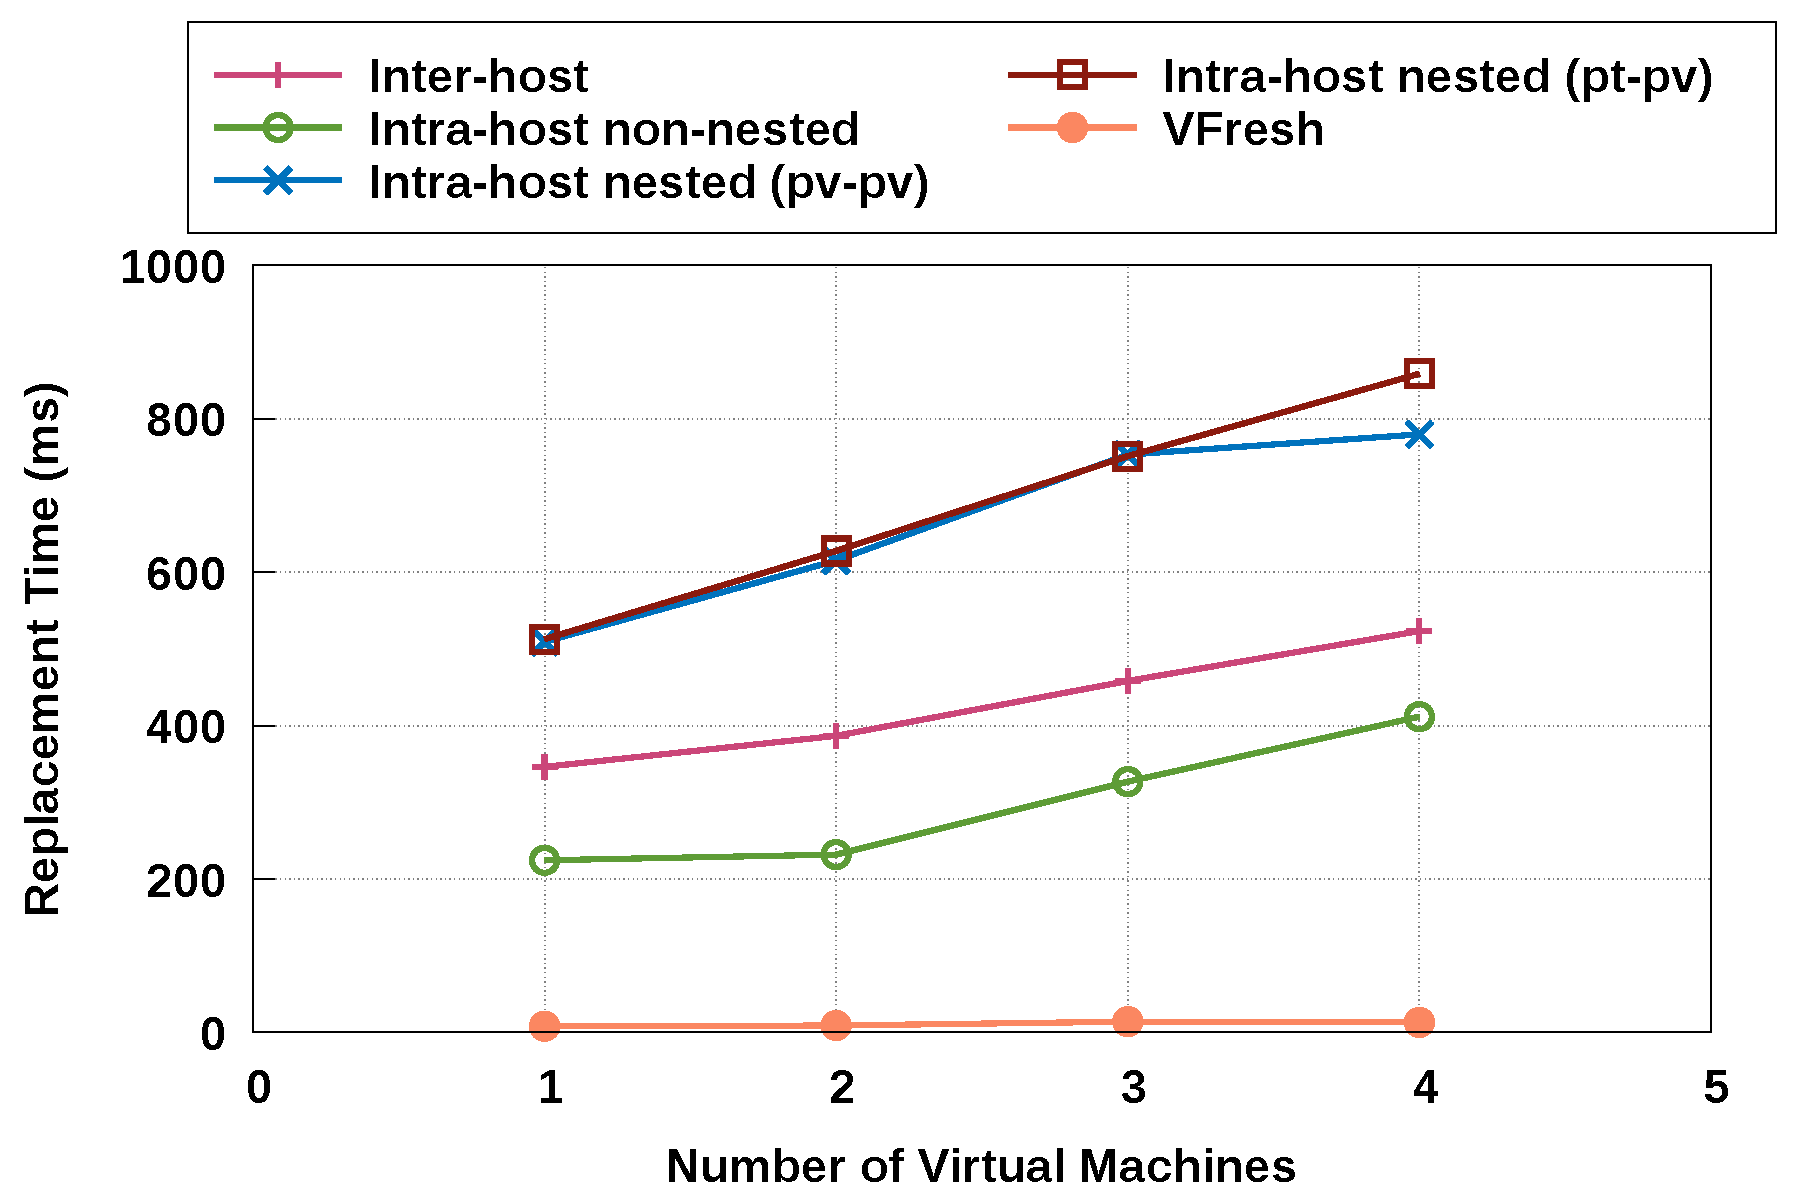
\includegraphics[width=.95\linewidth]{figures/multivm_idle_guest_migration_vFresh.pdf}
   \vspace{-0.1in}
  \captionof{figure}{Comparison of hypervisor replacement time for multiple idle VMs with varying VM \#.}
  \label{fig:multiVfreshIdle}
\end{minipage}
\hspace{0.34in}
\begin{minipage}{.43\textwidth}
  \centering
  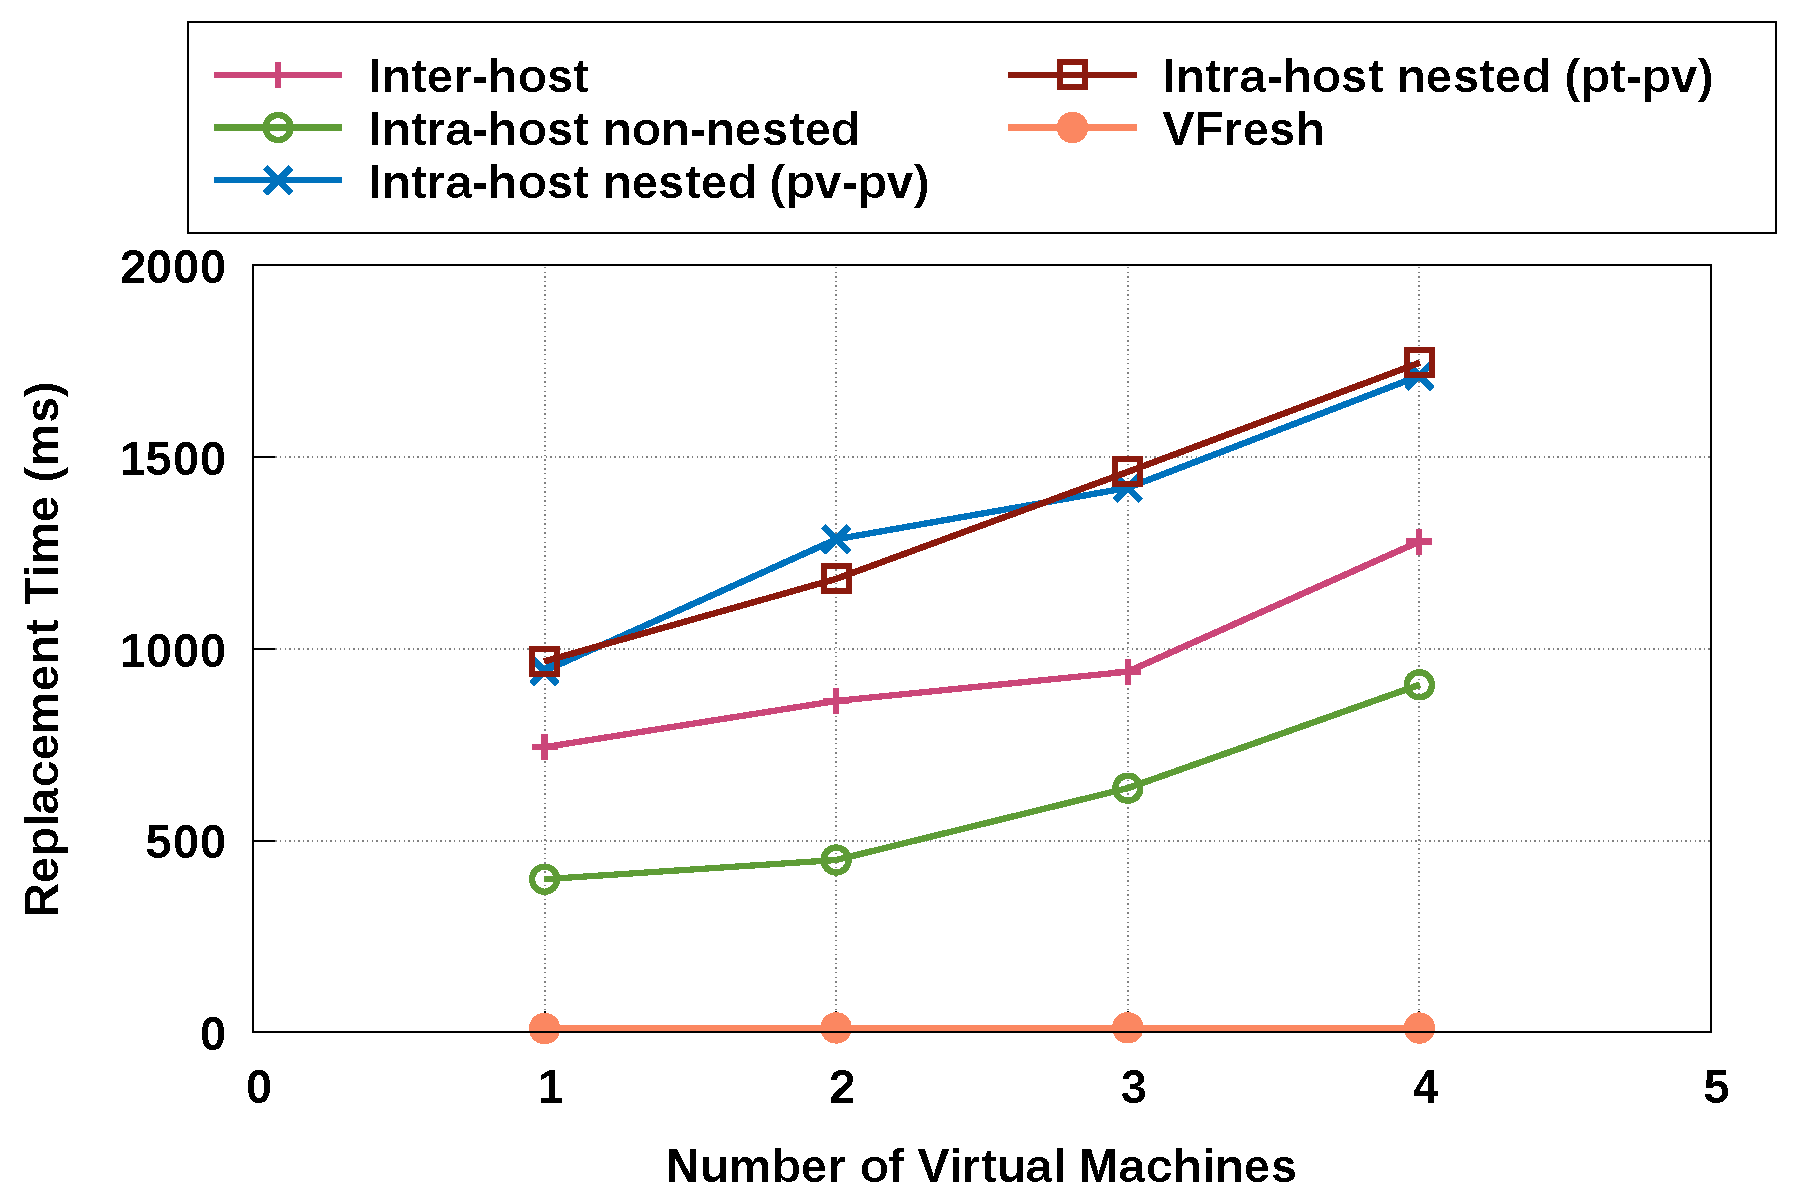
\includegraphics[width=.95\linewidth]{figures/multivm_busy_guest_migration_vFresh.pdf}
   \vspace{-0.1in}
  \captionof{figure}{Comparison of hypervisor replacement time for multiple write-intensive VMs with varying VM \#.}
  \label{fig:multiVfreshBusy}
\end{minipage}%
  \vspace{-0.1in}
\end{figure*}

\begin{table}
\small
\begin{tabular}{|p{1.75cm}|p{1.65cm}|p{1.5cm}|p{1.5cm}|} \hline
 & Hyperplexor & Hypervisor & Guest \\ \hline
Host & 1GB, \linebreak 1CPU & - & - \\ \hline
Non-Nested & 8GB, \linebreak 4CPUs & - & 1GB, 1VCPU \\ \hline
Nested & 32GB, 10CPUs & 8GB, \linebreak 4VCPUs & 1GB, 1VCPU \\ \hline
\arch & 32GB, 10CPUs & 8GB, \linebreak 4VCPUs & 1GB, 1VCPU \\ \hline
\end{tabular}
\vspace{6pt}
\caption{Experiment setup to measure the hypervisor replacement time for different setups.}
\label{tab:setup1}
\end{table}


\subsubsection{Replacement Time}
We measure the hypervisor replacement time under \arch and compare it with 
%optimized pre-copy migration. 
the four cases based on the optimized pre-copy live migration as stated in Section \ref{sec:motiv}, which are (a) inter-host, (b) intra-host nested (pv-pv), (c) intra-host nested (pt-pv), and (d) intra-host non-nested. The nested virtualization configurations are listed in detail in Table \ref{tab:setup1}: The L2 VMs are configured with 1 VCPU (and varying memory sizes under different test cases); the L1 hypervisors are configured with 8 GB memory and 4 VCPUs; and the L0 hyperplexor is configured with 32 GB memory and 10 CPUs. 

\para{Single VM.} First, we use a single idle VM and vary its memory sizes from 1 GB to 4 GB. \fref{fig:idleVfresh} shows that the total replacement time under the inter-host case is around 0.35 seconds for 1 GB memory and 0.6 seconds for 4 GB memory. Under the intra-host nested cases (both pv-pv and pt-pv), the replacement time increases to around 0.5 seconds for 1 GB memory, and 1.17 seconds for 4 GB memory. In contrast, the total hypervisor replacement time under \arch is extremely low --- 10 ms. Further, the replacement time remains constant as the VM's memory size increases. It is because, in \arch, the memory is re-mapped between the L1 hypervisors and such operations are performed out of the critical path of the VM state transfer; the replacement time only comprises of the time of transferring the VCPU and I/O device state information, which is constant. 
%the total replacement time is almost constant and independent of the VM memory size. Instead, the replacement time only comprises of the time of transferring the VCPU and I/O device state information. 
%The migration rate limit, pre-copy iterations and the page dirty rate do not affect the total migration time in \arch.  
However, under both the inter-host and intra-host cases, transferring the memory pages through the network accounts for higher total migration time and thus higher replacement time. 

%Explain what is working set
%dirty page rate is 50000pages/second
Next, we use a busy VM with varying memory sizes. The busy VM runs a ``working set'' benchmark which dirties the memory at a controllable page dirty rate --- we fix it as 5,000 pages per second in all our experiments.
%As explained before, working set is a write-intensive synthetic benchmark 
%with varying sizes of memory at a fixed dirty rate --- 5,000 pages per second. \
In \fref{fig:VfreshBusy}, under all pre-copy live migration based cases the replacement time again increases as the memory size of the VM increases. The replacement time is higher than that under the idle VM, because dirtied pages are transferred in multiple rounds for the busy VM.
With \arch, the replacement time remains constant irrespective of the memory dirty rate --- the replacement time remains around 10 ms for the cases with varying memory sizes.
%with increase in size of the working set as the number of dirty pages to be transferred in pre-copy iterations increase. 
%The increase in total migration time for nested guest is due to the overhead introduced by nested virtualization. 

%Busy guest	Memory Variation			
%							1		2		3		4
%Inter-host					743.6	1433	1975.8	2342.6
%Intrahost non-nested		399.6	730.6	1020	1190
%Intrahost nested(pv-pv)	942.4	1750	2634	3170
%Intrahost nested(pv-pt)	967.4	1770.6	2623.2	3241.6
%Hyperfresh					10		9		10.2	9.4


%\begin{figure}
%	\centering
%	\subfloat[Idle guest]{
%		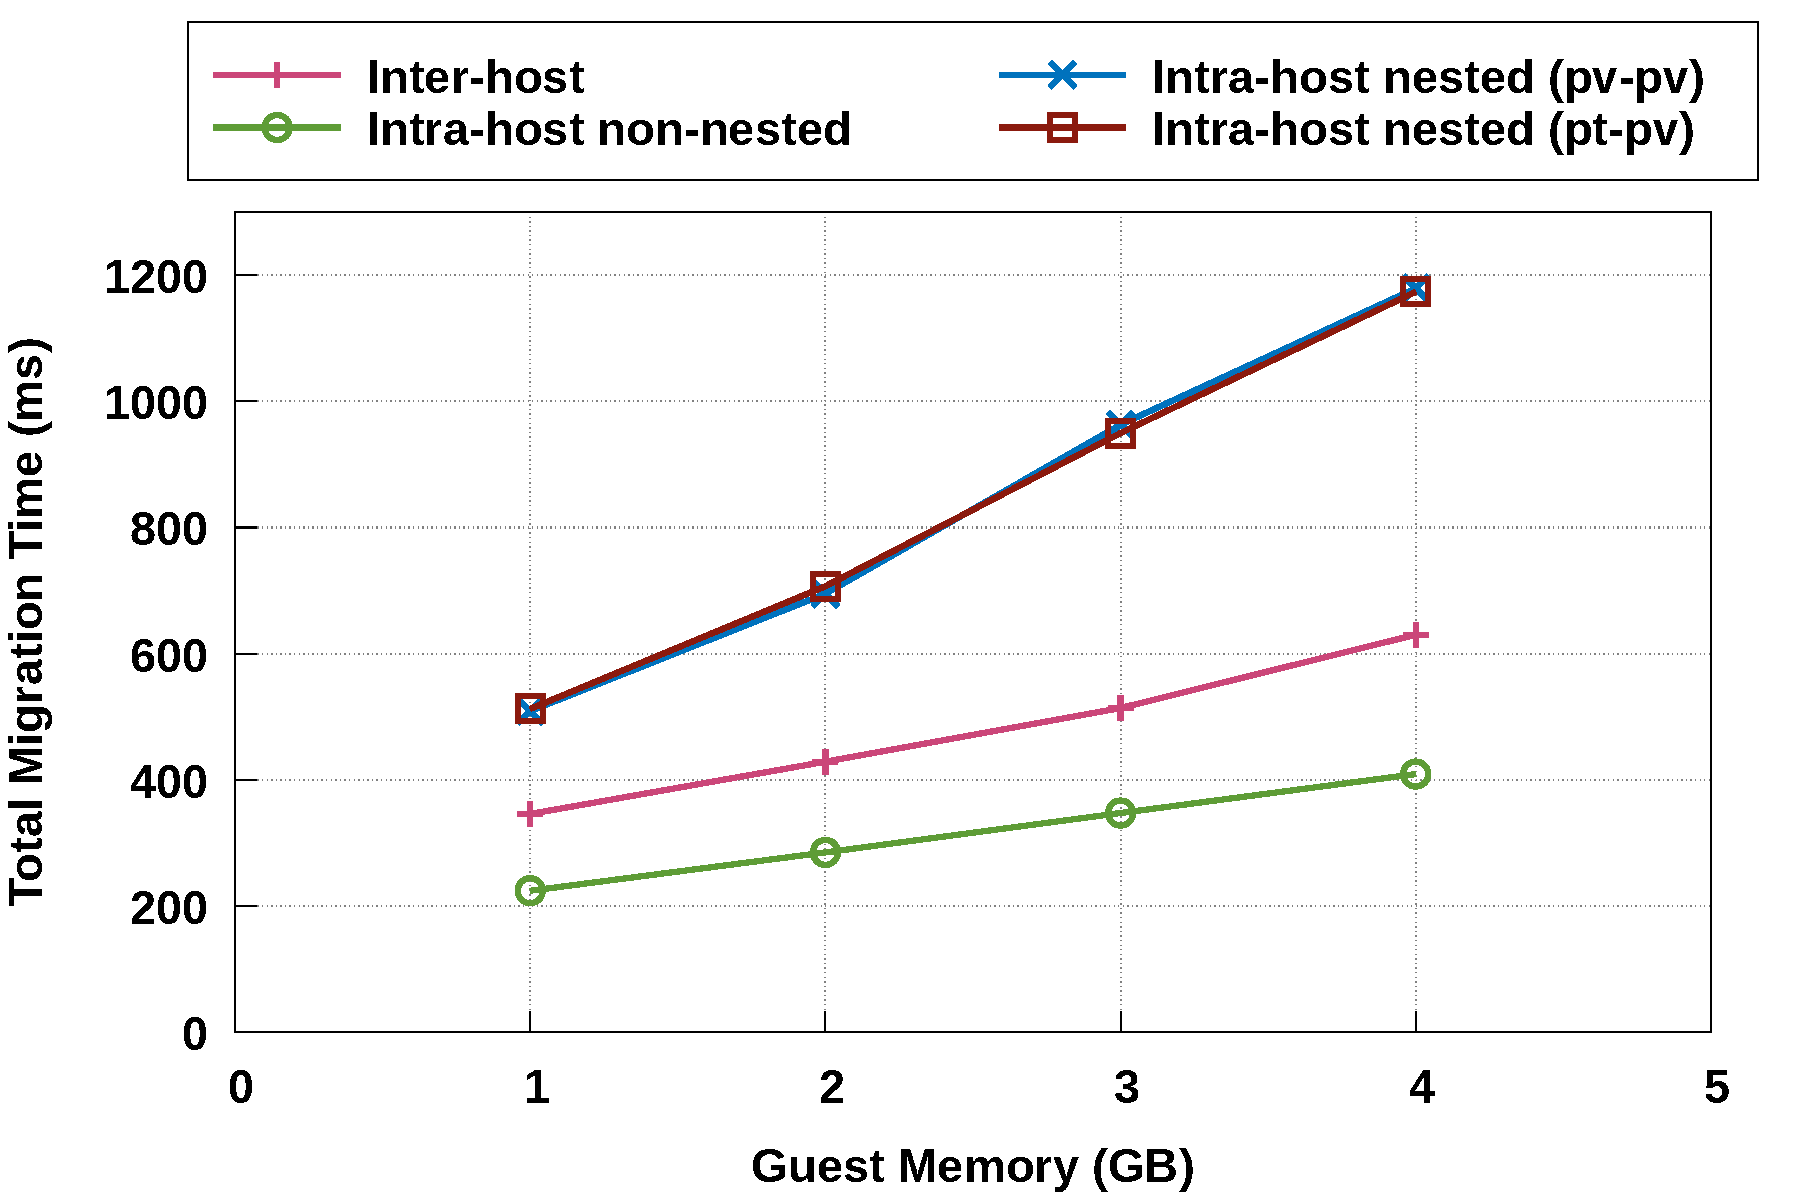
\includegraphics[width=.235\textwidth]{figures/idle_guest_migration.pdf}}
%	\subfloat[Busy guest]{
%		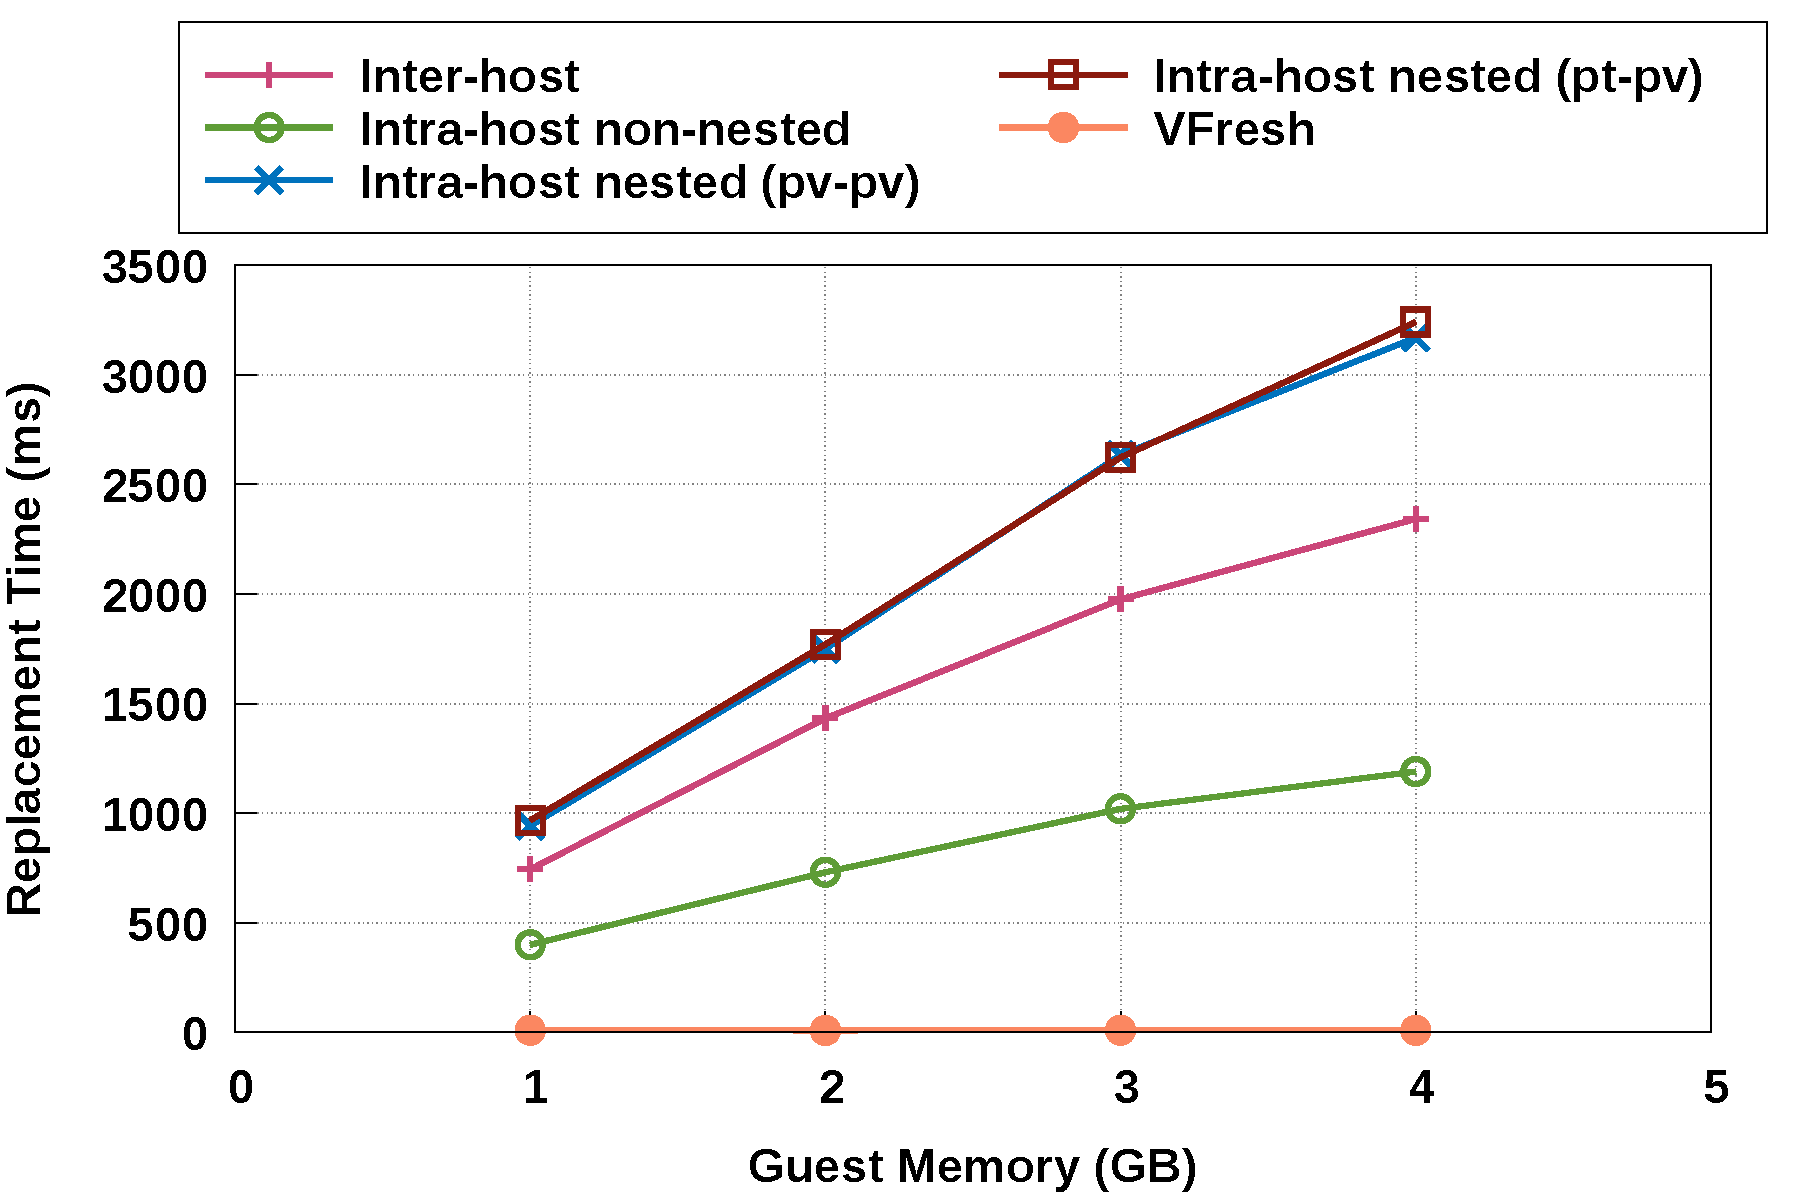
\includegraphics[width=.235\textwidth]{figures/busy_guest_migration_with_vFresh.pdf}}
%	\caption{Replacement time comparison with VFresh}
%	\label{fig:rt_exp1}
%\end{figure}

\para{Multiple VMs.} 
Further, we measure the replacement time
%to replace old hypervisor with new hypervisor that is 
by running multiple VMs on the same stale hypervisor and later moving them to another co-located replacement hypervisor. We vary the VM number from 1 to 4. 
Each VM is configured with 1 GB memory; all the VMs start the migration at the same time. 
We consider the following two cases: (1) with all VMs being idle and (2) with all VMs being busy (with the same page dirty rate of 5,000 pages per second). 

In \fref{fig:multiVfreshIdle}, with all idle VMs, it takes 0.3 seconds to migrate 1 VM and 0.5 seconds to migrate 4 VMs under inter-host live migration. The migration time increases to 0.5 seconds for migrating 1 VM and 0.8 seconds for 4 VMs under intra-host nested live migration (for both pv-pv and pt-pv setups). In \fref{fig:multiVfreshBusy}, with all busy VMs, it takes 0.7 seconds to migrate 1 VM and 1.27 seconds for 4 VMs under inter-host live migration. Under intra-host nested live migration (for both pv-pv and pt-pv setups), the migration time increases to 1 second for 1 VM and 1.75 seconds for 4 VMs.
In contrast, with \arch, the time to replace the hypervisor remains 10 ms with either idle or busy VMs. The replacement time does not increase as the number of VMs increases, because again the VMs' memory is remapped and only the VCPU and I/O device state is transferred during hypervisor replacement.
%from one host to another using optimized pre-copy and it takes 0.3s to migrate 1 VM and increases to 0.5s to migrate 4 virtual machines. The migration time increases when nested virtual machines are migrated from one hypervisor to another on the same host with both pv-pv and pt-pv setup. 
%In \fref{fig:multiVfreshBusy}, 
%we migrate virtual machines that perform write intensive workload. Every virtual machine dirties the memory at the rate 50000 pages/second. The virtual machines are migrated once 80\% of every VM's memory is dirtied simultaneously. The migration time for optimized pre-copy migration increases from 0.7 s to 1.27 s for 1 VM to 4 VMs. In \arch, the time to replace the hypervisor remains to be 10ms running busy or idle virtual machines. The replacement time does not increase with increase in number of virtual machines because the guest memory is co-mapped and only the VCPU and I/O device information is transferred during migration.

\begin{figure}
	\centering
	\subfloat[Optimized pre-copy]{
		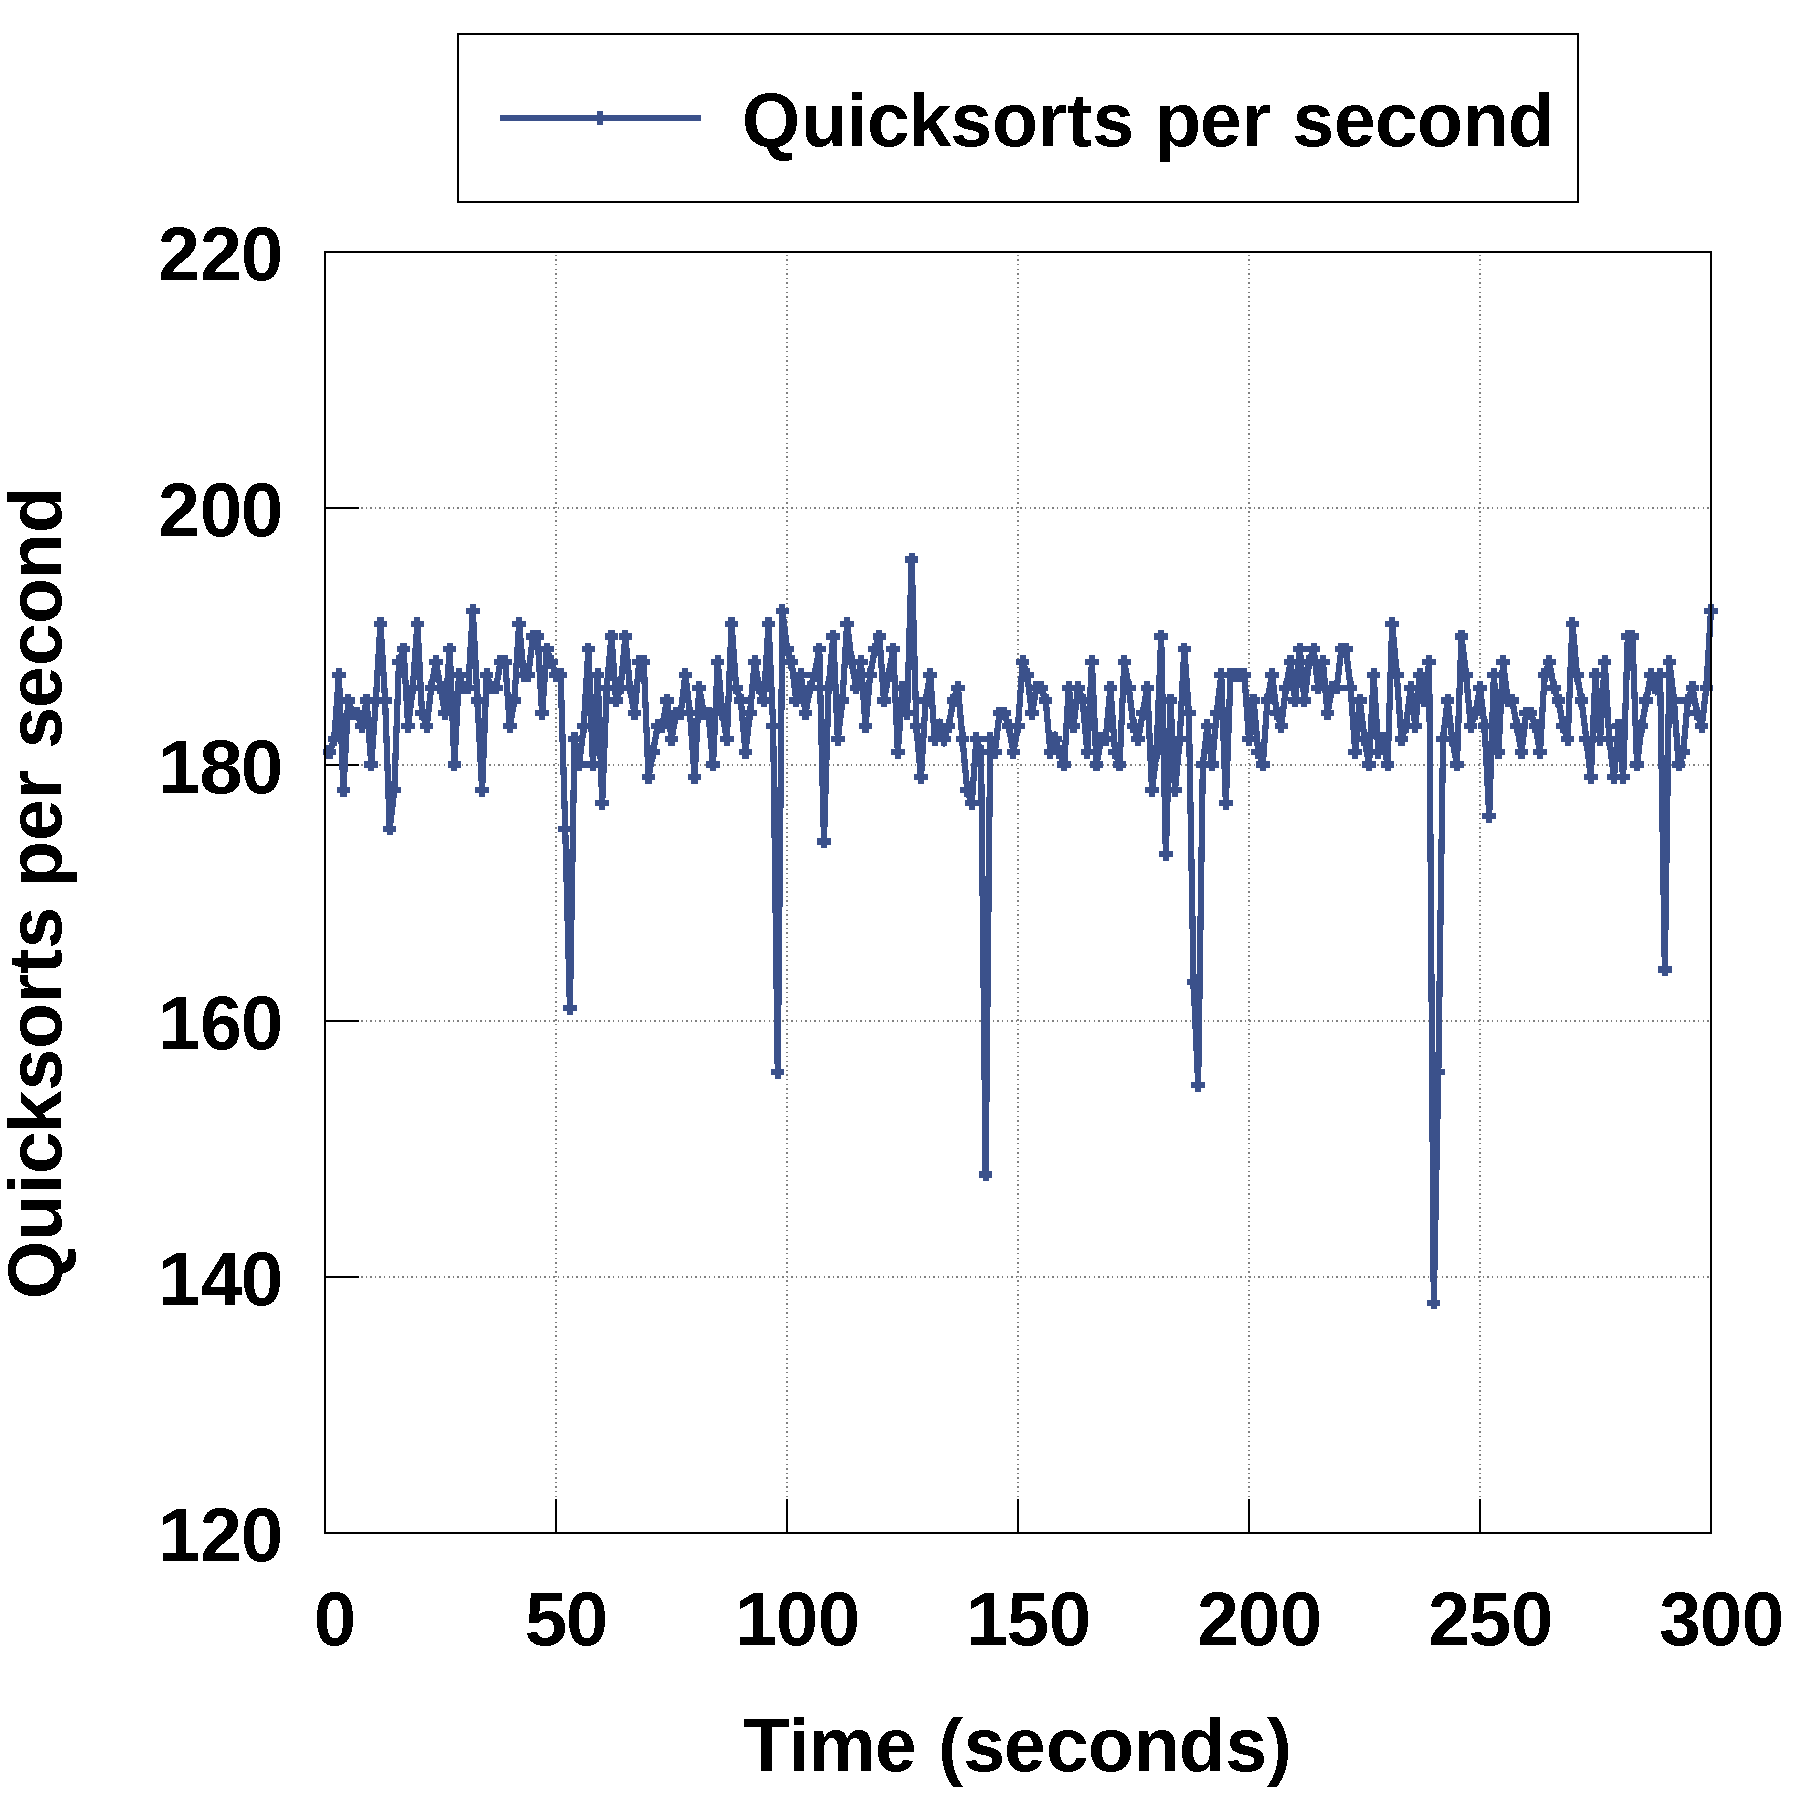
\includegraphics[width=.235\textwidth]{figures/qsortps_1GB_nested_precopy_disable_rate_limit.pdf}}
	\subfloat[\arch.]{
		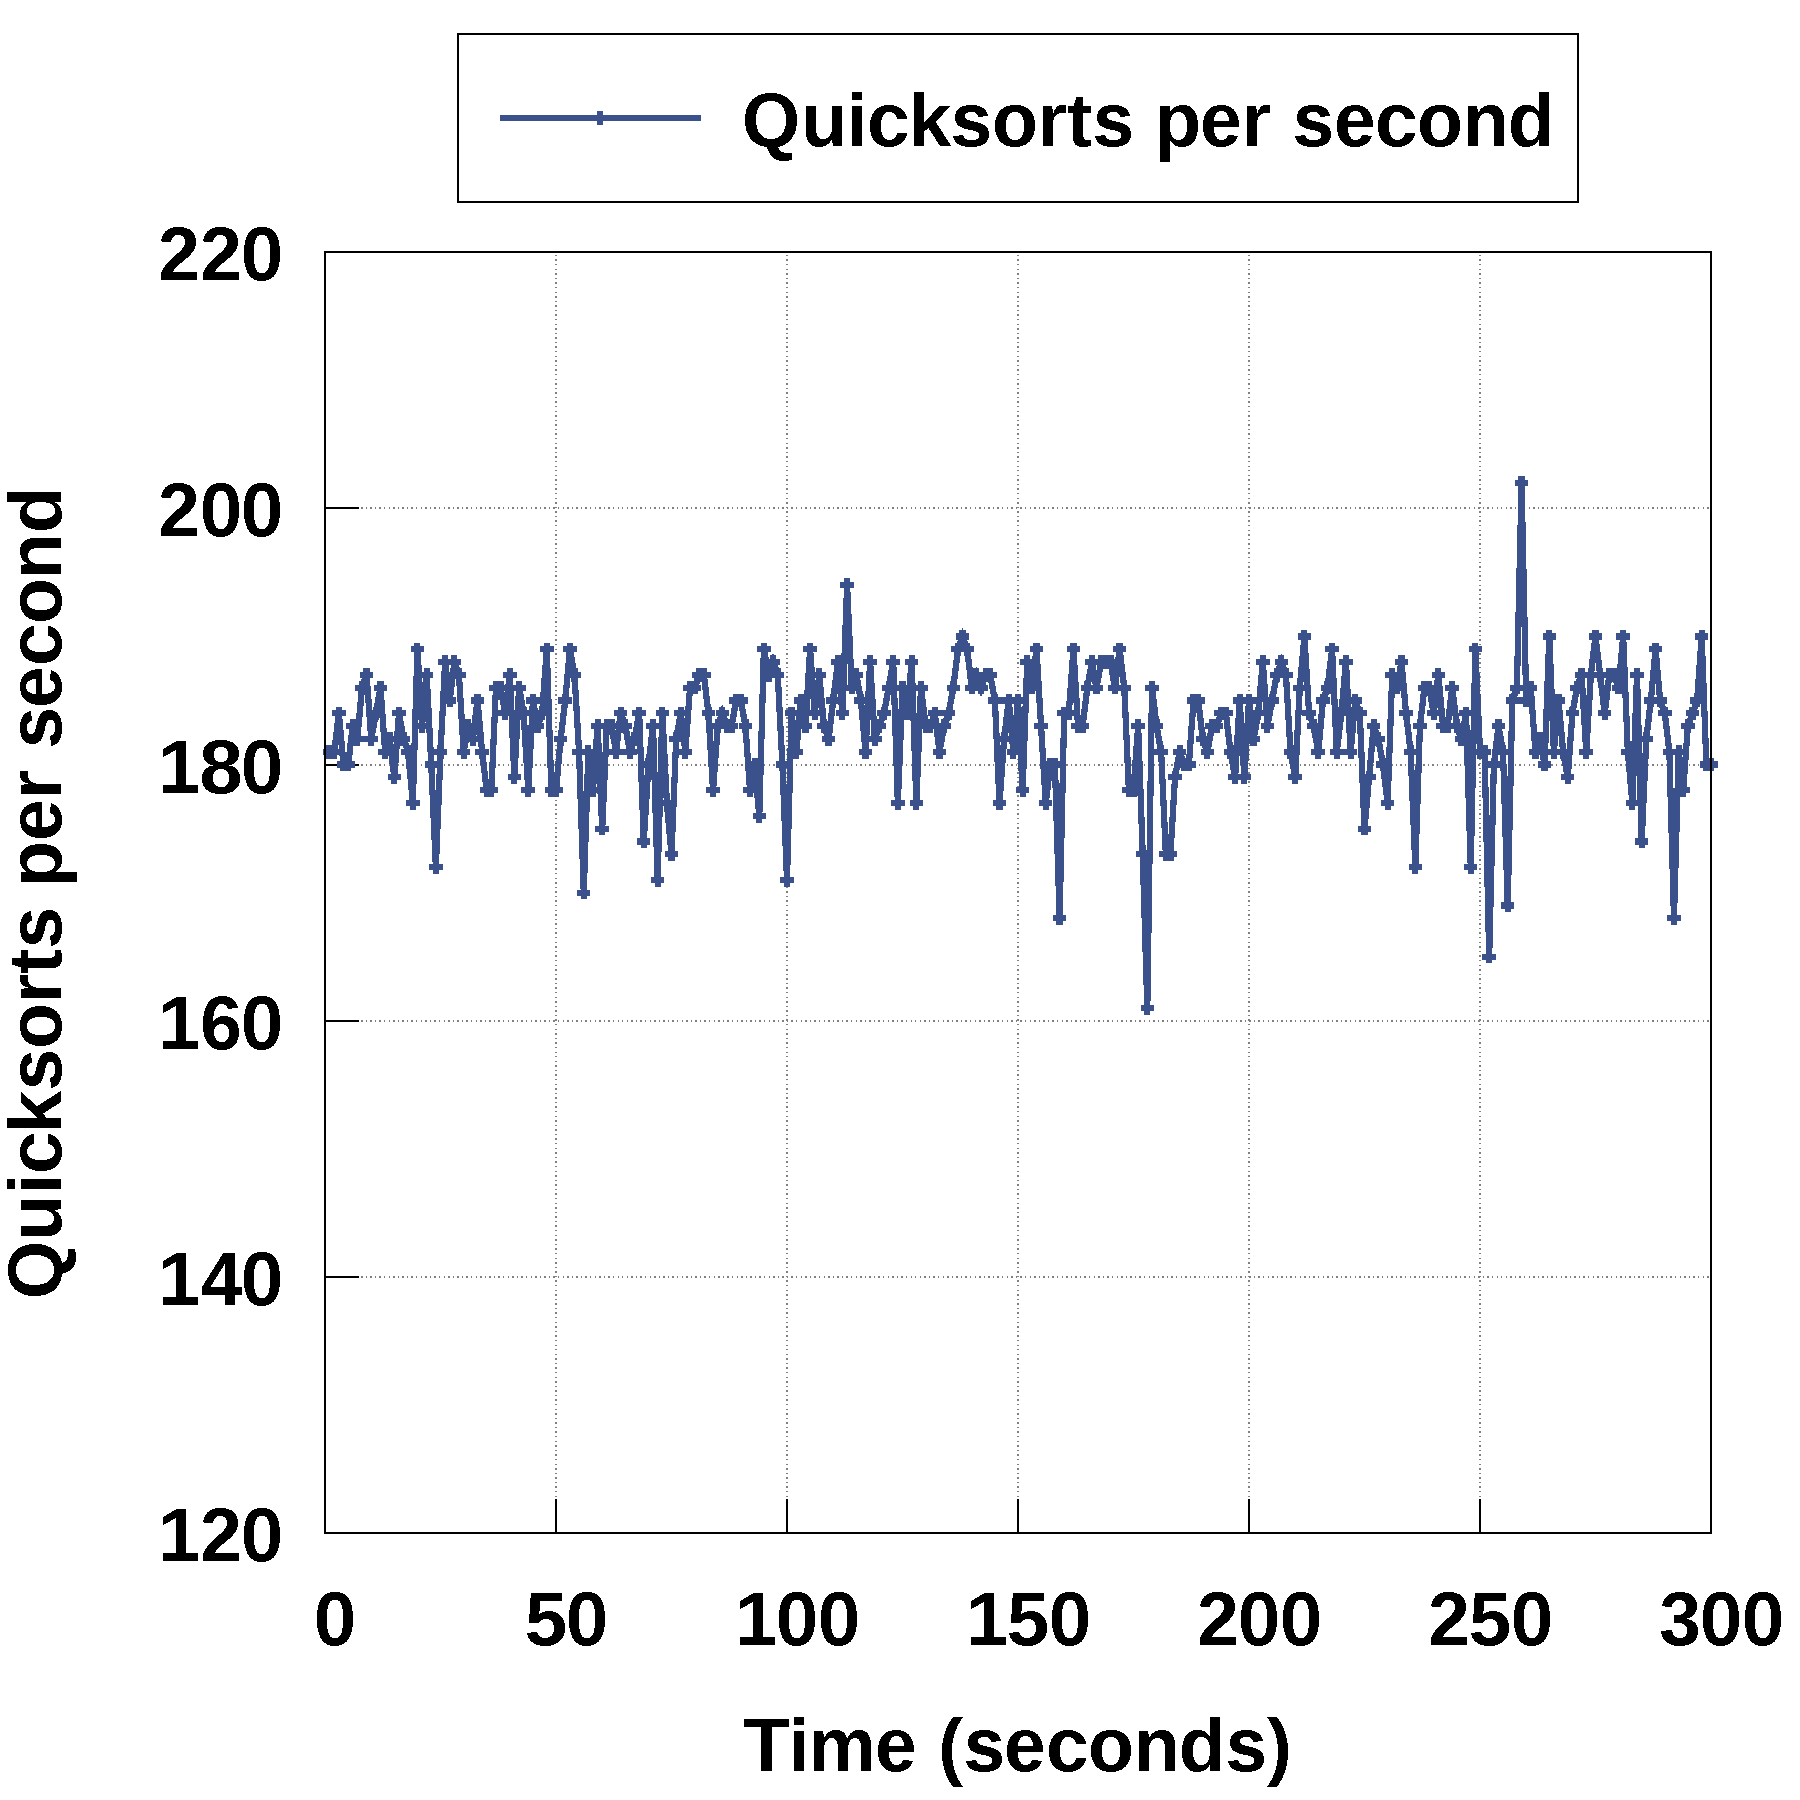
\includegraphics[width=.235\textwidth]{figures/qsortps_1GB_nested_precopy_hyperfresh.pdf}}
	\caption{Quicksort performance over multiple hypervisor replacements.}
	\label{fig:implq}
\end{figure}


%\begin{figure}
%	\centering
%   	\subfloat[Optimized Pre-copy migration]{
%		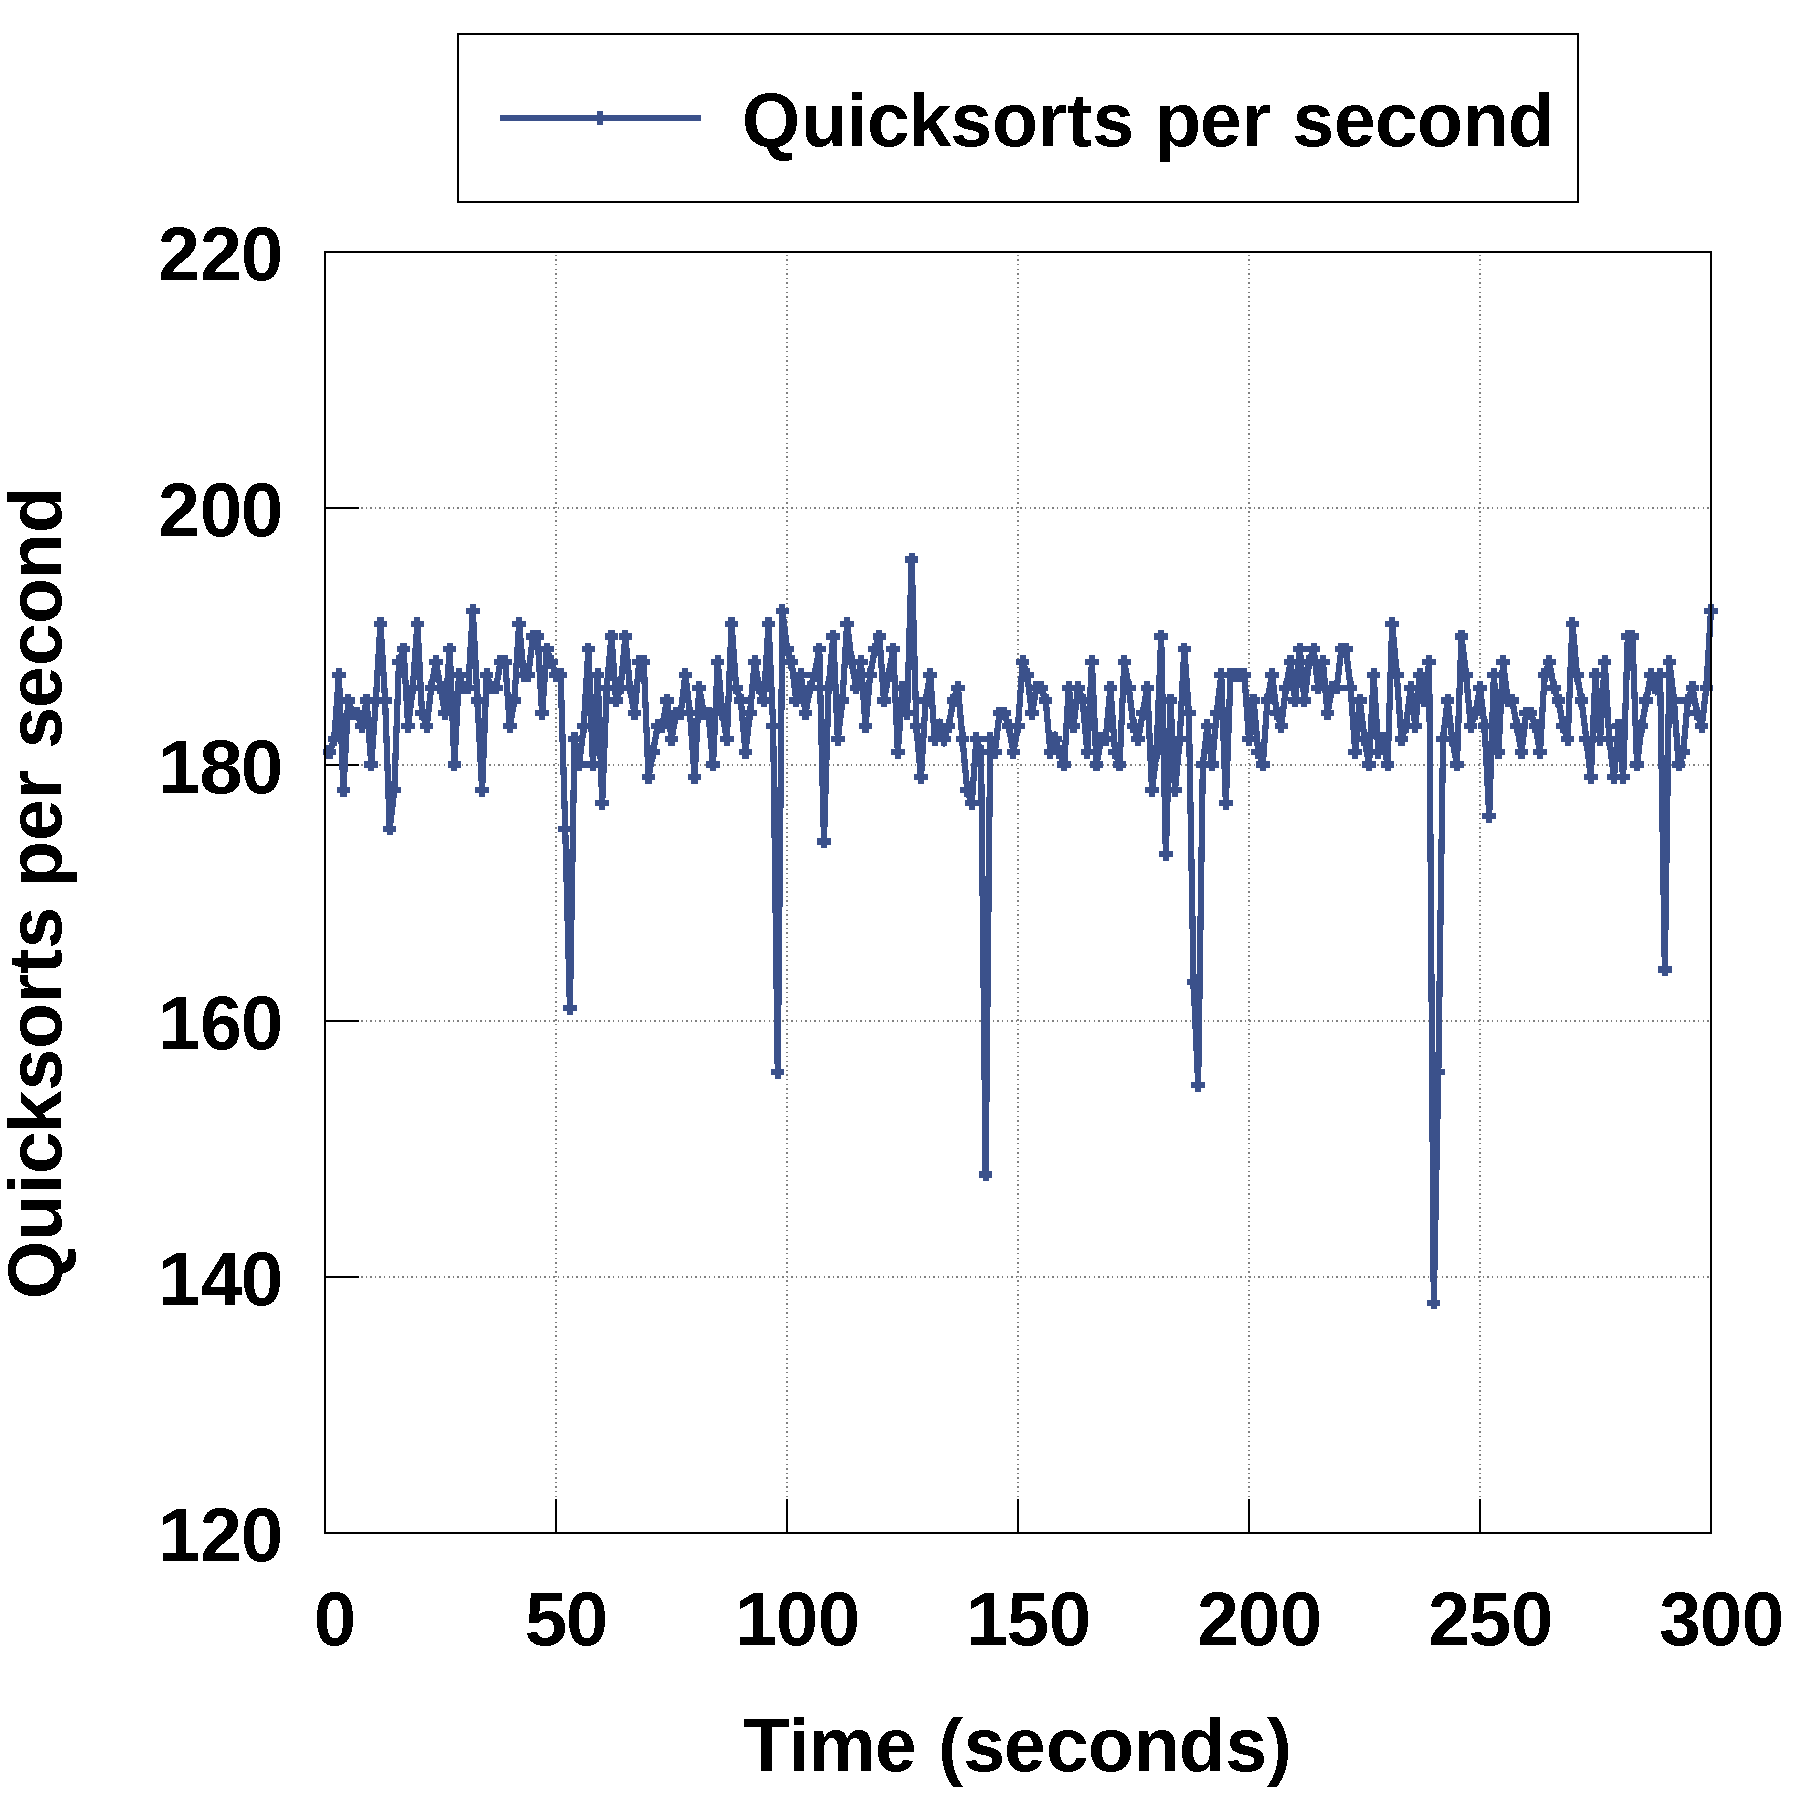
\includegraphics[width=.235\textwidth]{figures/qsortps_1GB_nested_precopy_disable_rate_limit.pdf}}
%		\hspace{0.1in}     
%	\subfloat[\arch]{
%		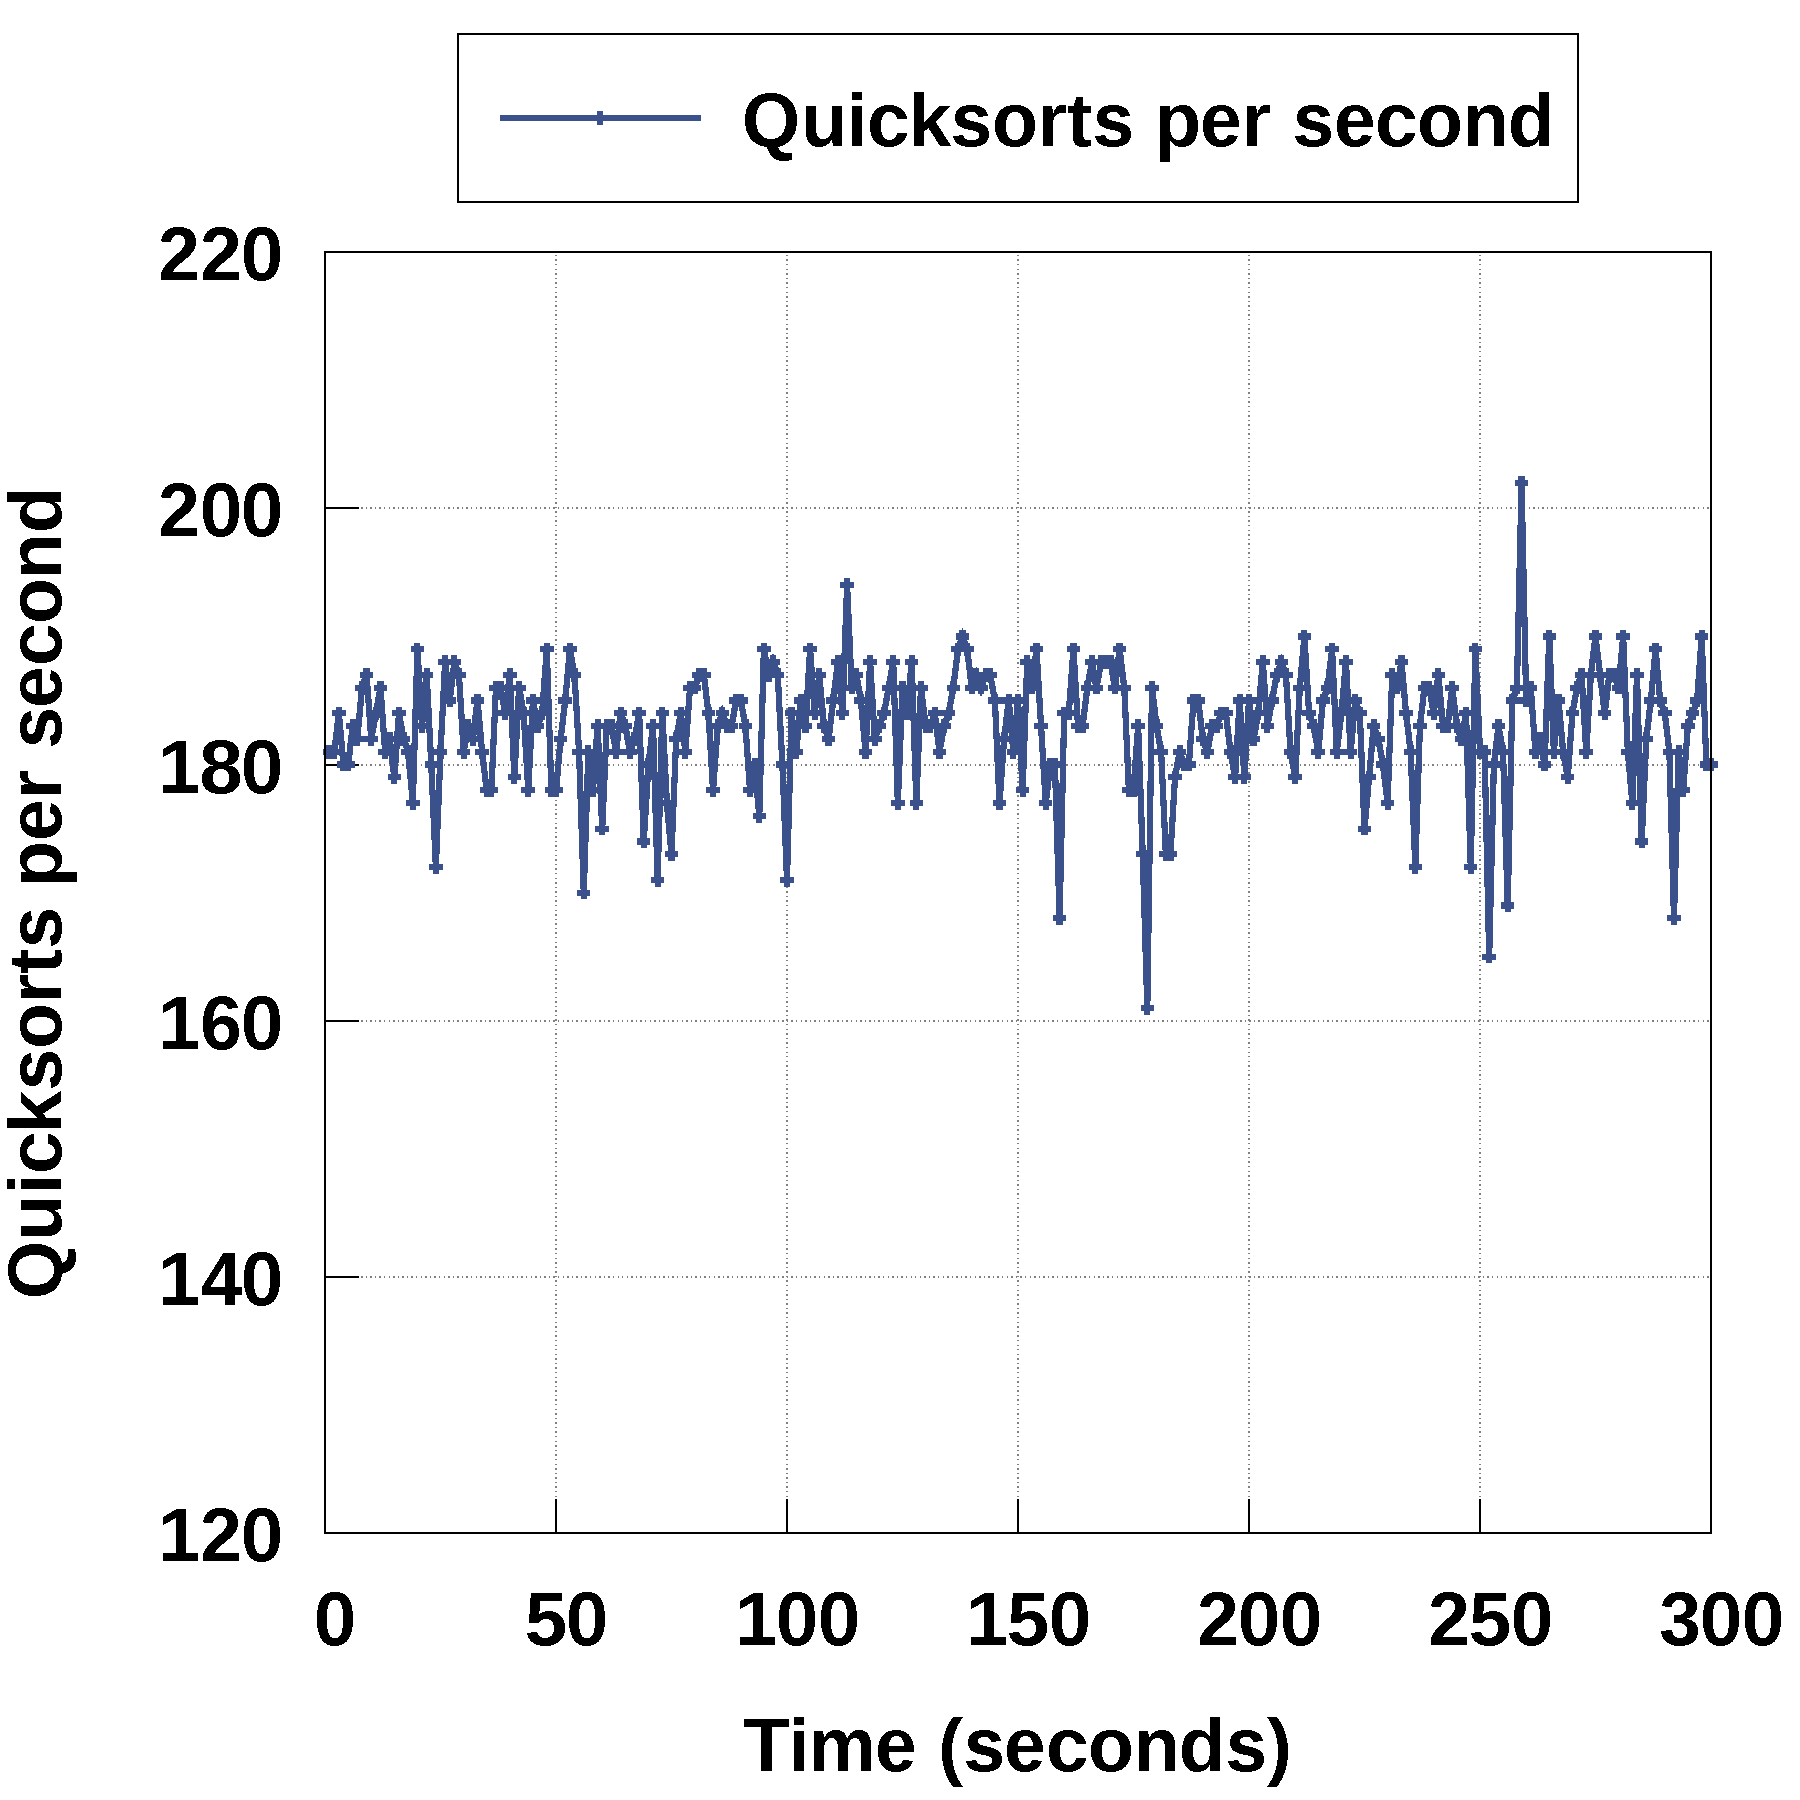
\includegraphics[width=.235\textwidth]{figures/qsortps_1GB_nested_precopy_hyperfresh.pdf}}
		%\hspace{0.1in}
%		\vspace{-0.1in}
%	\caption{Quicksort performance during migration of a nested guest: Optimized Pre-copy vs. VFresh}
%	\vspace{-0.1in}
%    \label{fig:impl}
%\end{figure}

\subsubsection{Performance Impact} 
We measure the application performance during hypervisor replacement between \arch and the intra-host nested (pt-pv) case. We use a CPU-intensive benchmark, Quicksort.
%The Quicksort benchmark is a CPU-intensive benchmark: 
Quicksort first allocates 1 GB memory, and then each operation takes 200 KB (50 pages) from the pre-allocated memory, writes random integers into it and performs the quicksort algorithm on these pages. In \fref{fig:implq}, we conduct 6 hypervisor replacements over a 300-second time window for both \arch and the intra-host nested case. We measure the number of quicksort operations per second during both regular execution and replacement.
%during migration of a nested VM using \arch and compare the results nested optimized pre-copy live migration.

%Idle guest	Number of Vms variation			
%Guest Memory (GB)			1		2		3		4
%Inter-host					346.2	386.6	458.2	523.2
%Intrahost non-nested		224.4	231.8	326.8	411.6
%Intrahost nested (pv-pv)	509.2	615.2	753.2	779.6
%Intrahost nested (pv-pt)	512.6	627.6	751.2	858.6
%Hyperfresh					8		9		14		13

%\begin{figure}[t!]
%  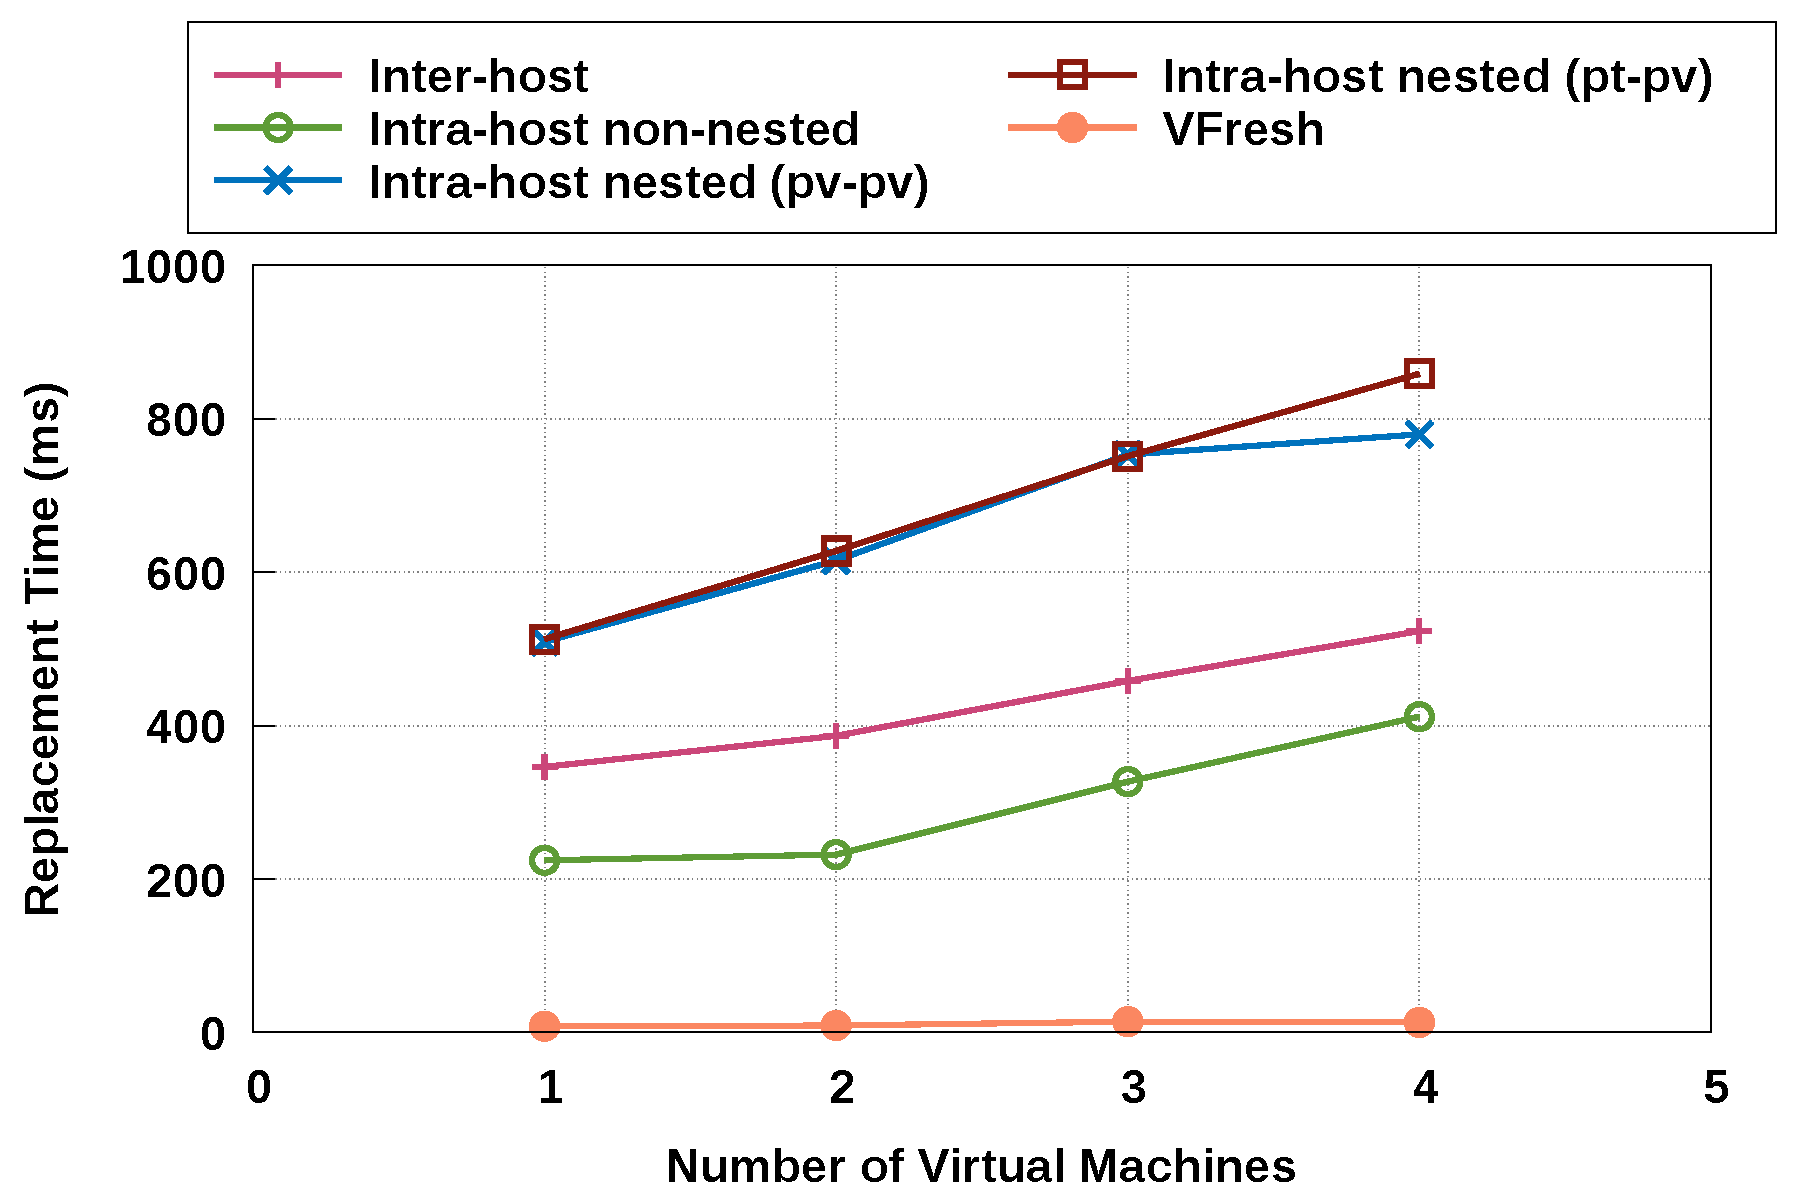
\includegraphics[width=0.45\textwidth]{figures/multivm_idle_guest_migration_vFresh.pdf}
%  \caption{Comparison of hypervisor replacement time for mutiple idle VMs with \arch and different setups.}
%  \label{fig:multiVfreshIdle}
%\end{figure}

%passthrough-vhost-net
%\fref{fig:impl1} shows that the performance of quicksort during optimized pre-copy migration. With optimized pre-copy, as the rate limit is disabled, a large number of dirty memory pages are transferred in less number of pre-copy iterations. As the number of pre-copy iterations decrease 
As shown in \fref{fig:implq}a, in the intra-host nested (pt-pv) case, there is no significant performance degradation during pre-copy iterations. However, the sharp performance dip is observed during the stop-and-copy phase, during which the VM is paused. 
%\fref{fig:impl}a. shows the dip in performance of quicksort during multiple optimized pre-copy migrations. 
In \fref{fig:implq}b, with \arch, the performance of quicksort does not reduce during the whole replacement and no significant performance dip is observed during the stop-and-copy phase. It is because, unlike the intra-host live migration case, \arch does not transfer any pages in the stop-and-copy phase, leading to much shorter stop-and-copy phase and hence less performance impact.   
%due to memory remapping


%Explain performance of quicksort during migration

%As discussed in the motivation section, the performance of the applications running in the guest decreases with decrease in the migration link bandwidth and the increase in bandwidth introduces significant network traffic during migration. In our solution, we eliminated the page transfer over the network and hence maintaining the performance of the applications in the guest. In Fig. 11 the performance of benchmark X does not get affected significantly during hypervisor refresh. 

%\begin{figure}[t!]
%  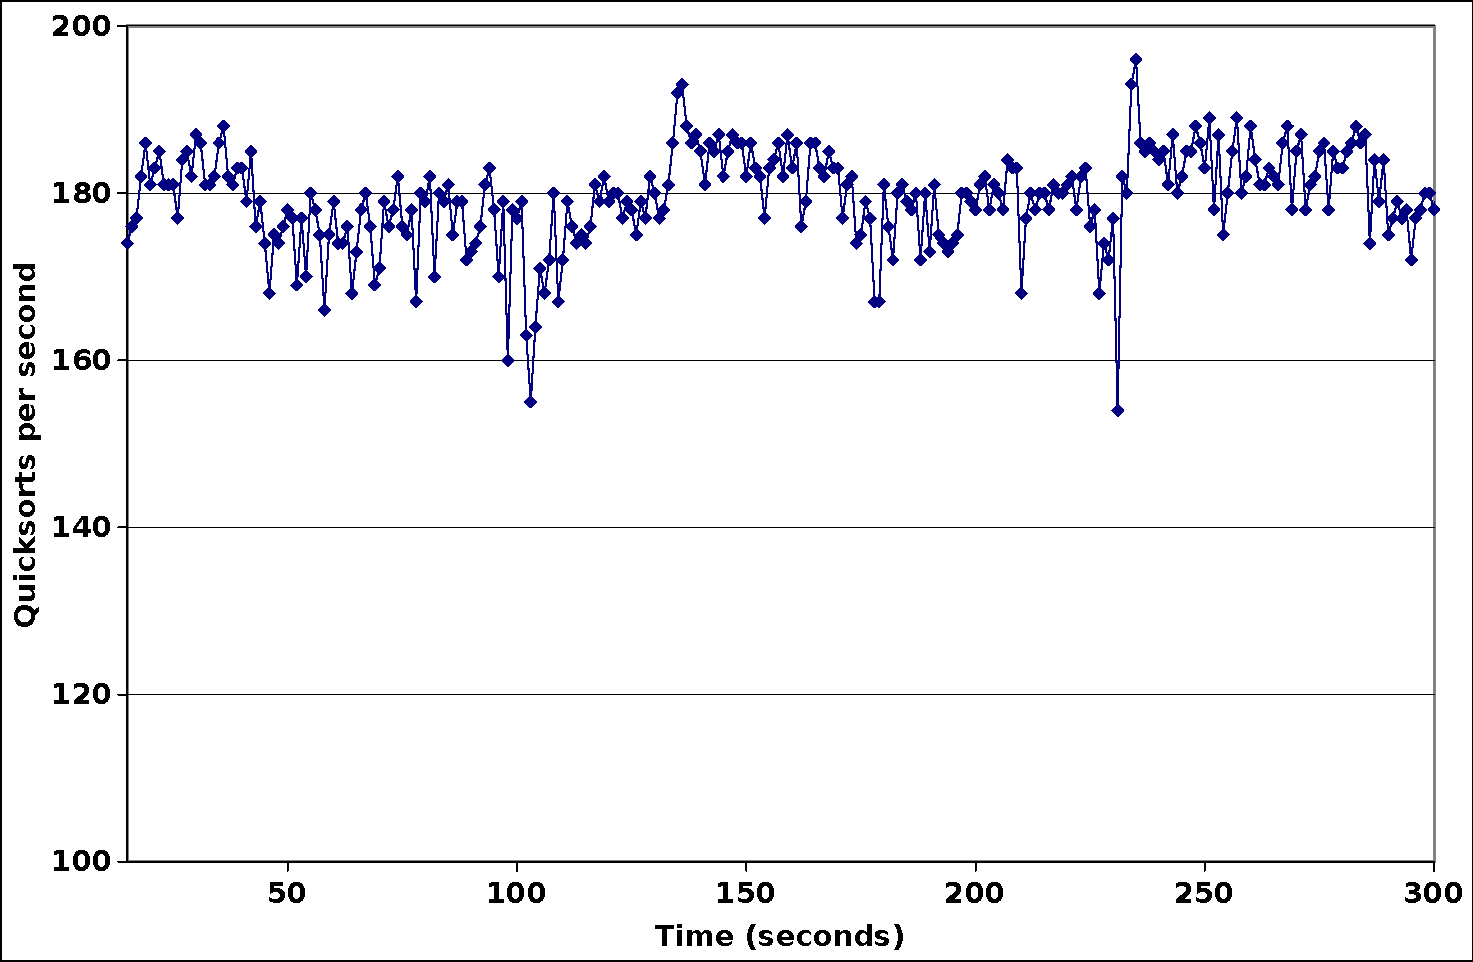
\includegraphics[width=0.5\textwidth]{figures/precopy-nested-2G-qsortps.pdf}
%  \caption{Pre-copy live migration: Performance of quicksort during migration of a %nested guest}
%  \label{quicksort-performance-1GB-nested-vhost-vhost.png}
%\end{figure}

%\subsubsection{Memory Mappings}
%The guest pages are pinned to the memory and populate the EPT and shadow EPT entries on boot up. The time taken to pin the pages in memory and populate the page table entries on the source host are 1.7 s, 3.3  s, 4.8 s, 6.3 s for a 1 GB, 2 GB, 3 GB and 4 GB memory respectively. The time taken on the destination host is 0.56 s, 1.2 s, 1.6 s, 2 s for 1 GB, 2 GB, 3 GB and 4GB respectively. The memory mapping time increases with increase in memory size of the guest as the number of pages to be mapped and hence the page table entries to be populated increase. The memory-mapping time measured represent the time taken to create the grant table used to transfer the memory mappings. The time taken to create the grant table increase with increase in guest memory as the number of hypercalls from hypervisor to hyperplexor increase along with grant table entries. However, this does not affect the total migration time as the grant table is created during the VM boot process.


%\begin{figure}[t!]
%  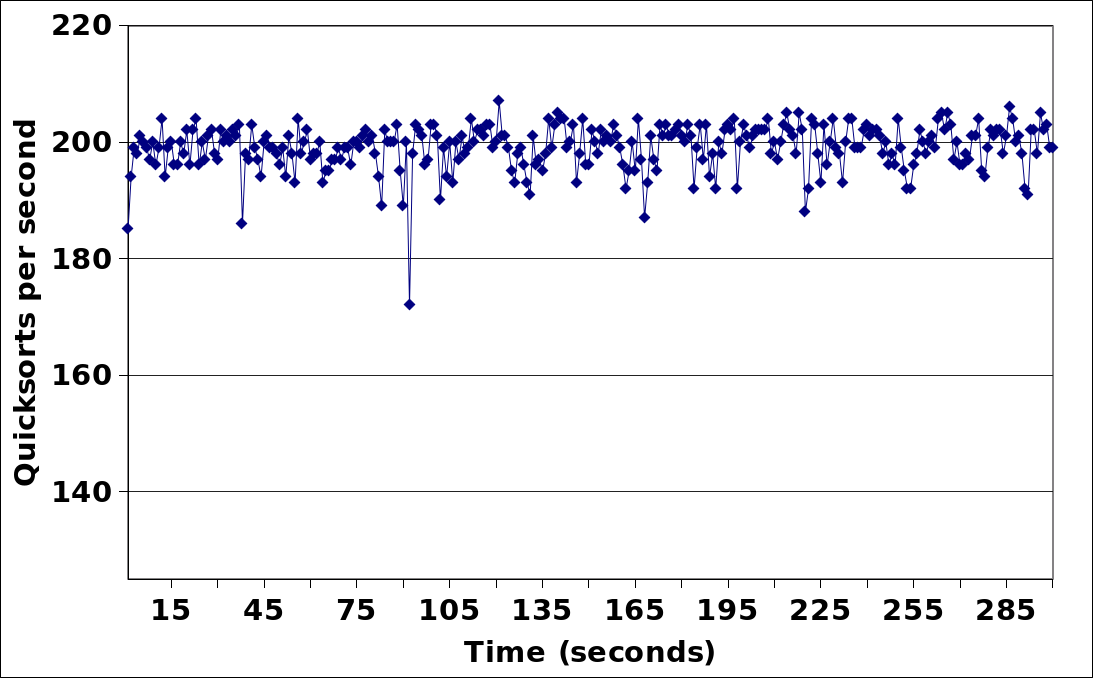
\includegraphics[width=0.5\textwidth]{figures/inter-host-quicksort-1GB.png}
%  \caption{Performance of quicksort during migration of guest from one host to another}
%  \label{quicksort-performance-1GB-interhost}
%  %\includegraphics[width=15cm,height=6cm,keepaspectratio]{architecture__1_.jpg}
%\end{figure}

%\begin{figure}[t!]
%  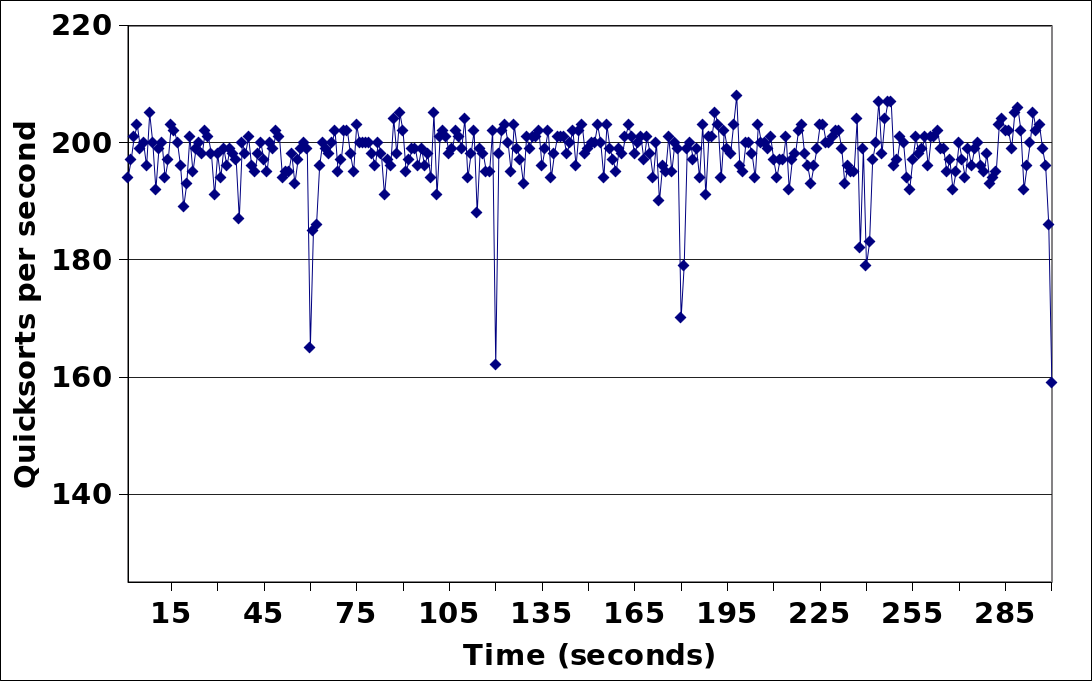
\includegraphics[width=0.5\textwidth]{figures/intrahost-non-nested-quicksort-1GB.png}
%  \caption{Performance of quicksort during migration of non-nested guest on same host}
%  \label{quicksort-performance-1GB-intrahost.png}
%  %\includegraphics[width=15cm,height=6cm,keepaspectratio]{architecture__1_.jpg}
%\end{figure}

%\begin{figure}[t!]
%  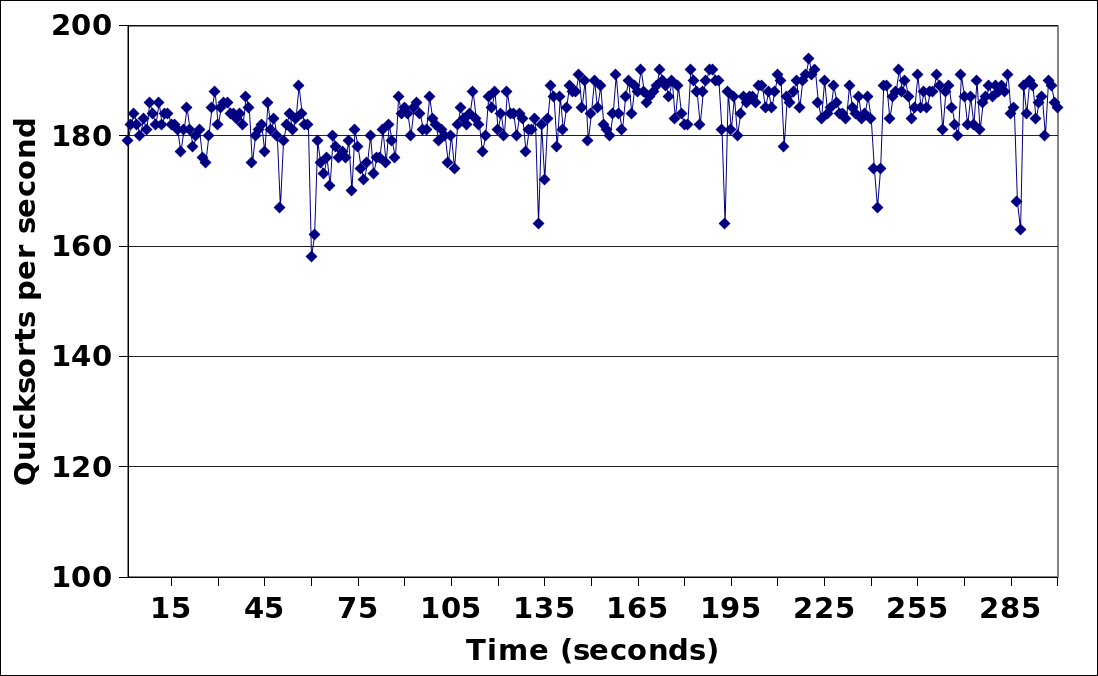
\includegraphics[width=0.5\textwidth]{figures/intrahost-nested-paravirt-quicksort-1GB.png}
%  \caption{Performance of quicksort during migration of a nested guest in para-virtualization %setting}
%  \label{quicksort-performance-1GB-nested-vfio-vhost.png}
%  %\includegraphics[width=15cm,height=6cm,keepaspectratio]{architecture__1_.jpg}
%\end{figure}

%\begin{figure}[t!]
%  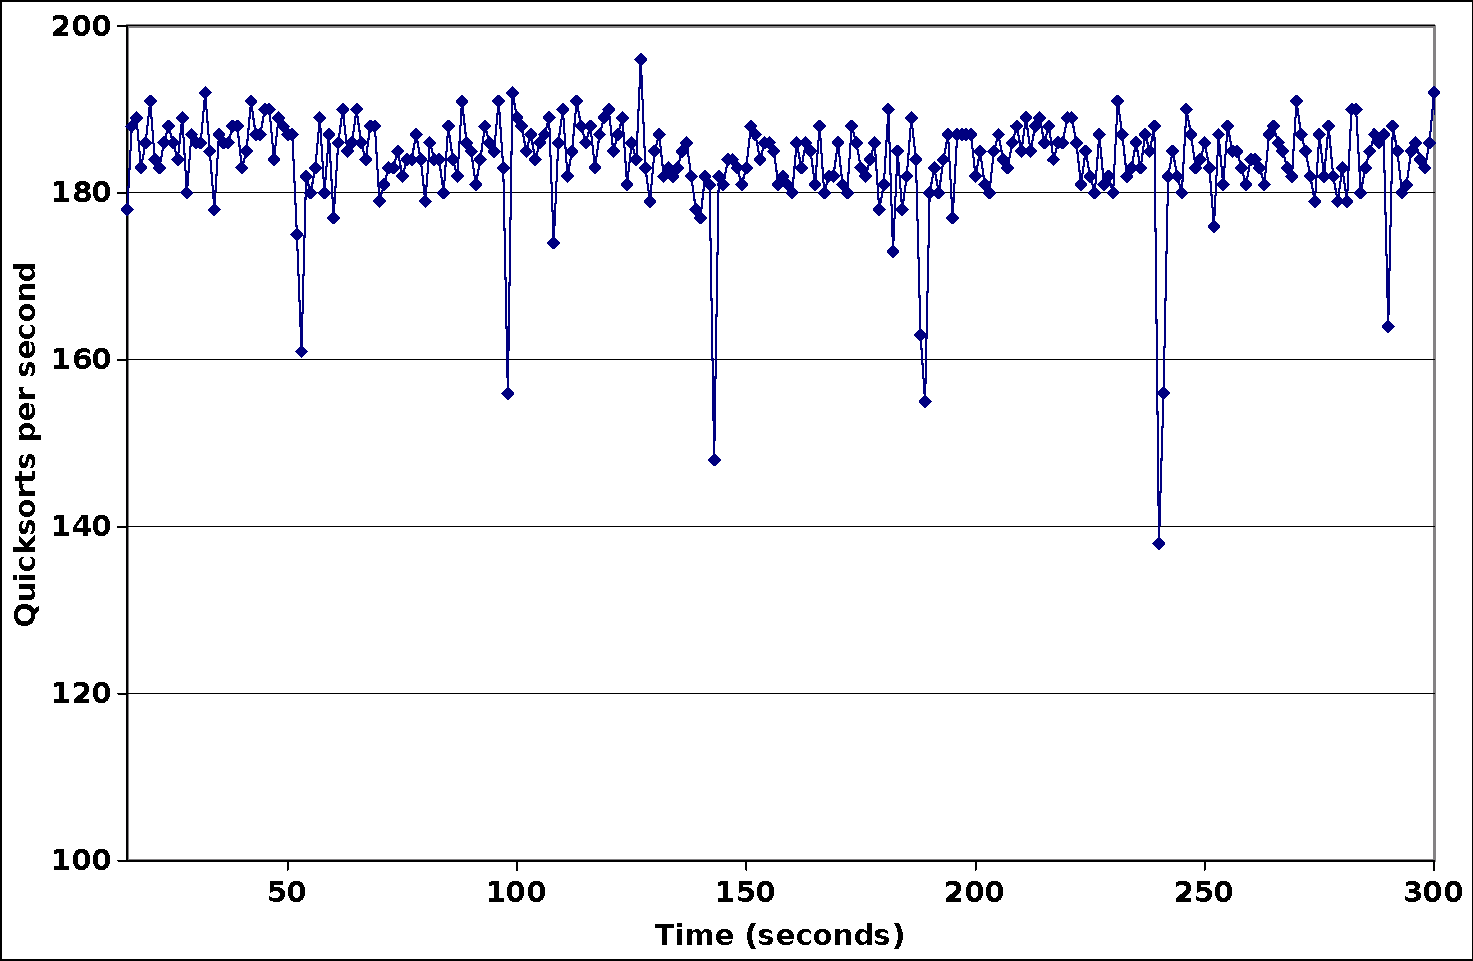
\includegraphics[width=0.5\textwidth]{figures/disable-rate-limit-pre-copy-qsortps-2G.pdf}
%  \caption{Optimized pre-copy live migration: Performance of quicksort during migration of a nested guest}
%  \label{quicksort-performance-1GB-nested-vhost-vhost2.png}
%\end{figure}

%\begin{figure}[t!]
%  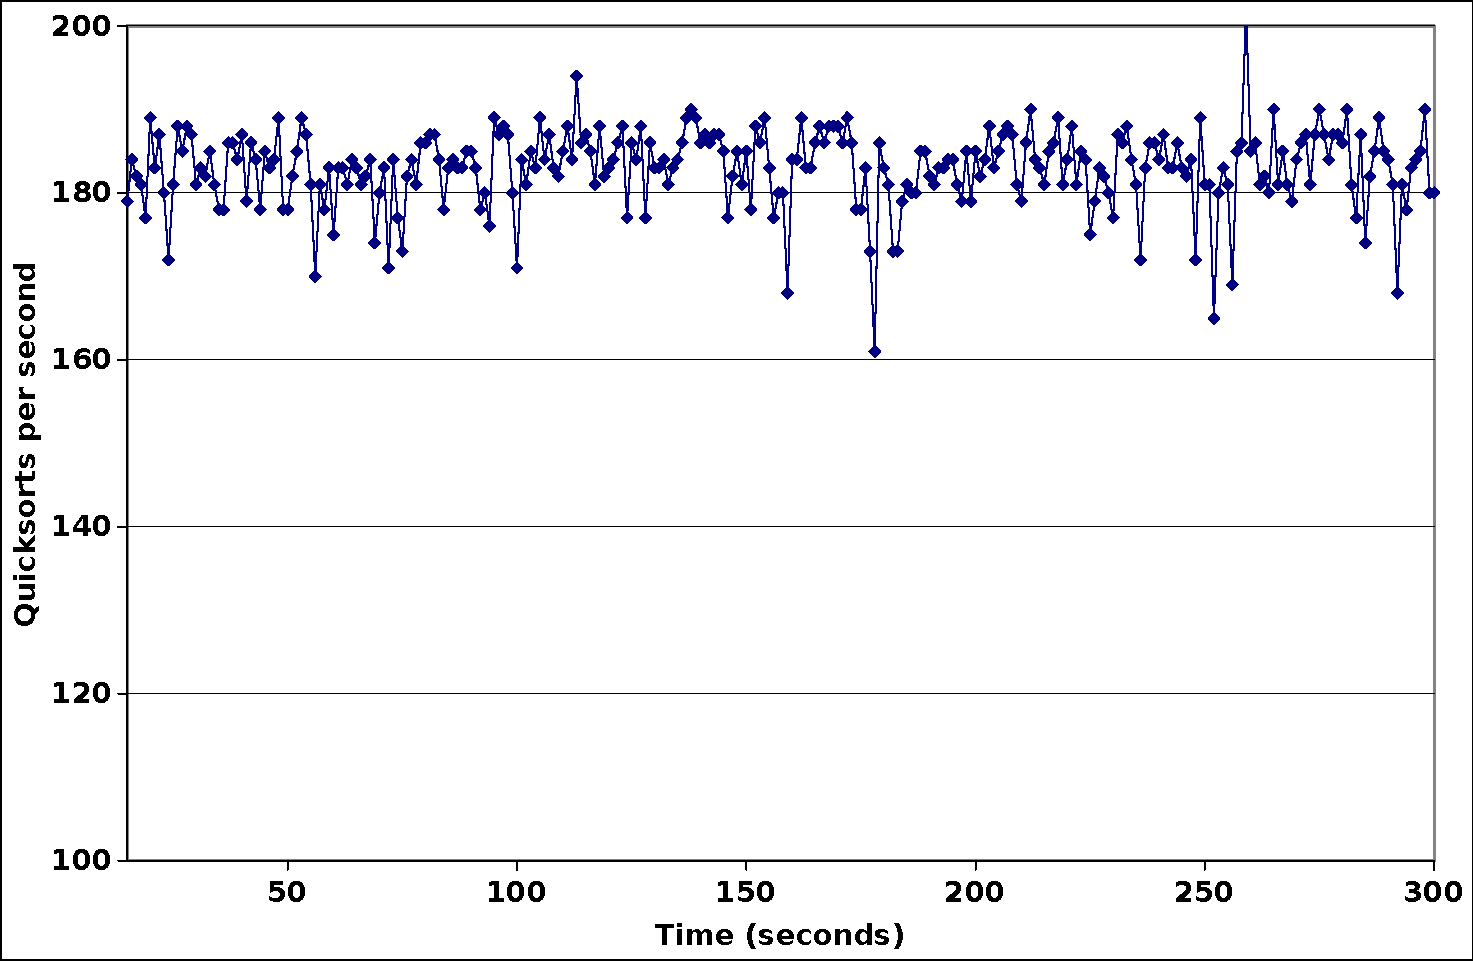
\includegraphics[width=0.5\textwidth]{figures/hyperfresh_qsortps_2G.pdf}
%  \caption{Hyperfresh: Performance of quicksort during migration of a nested guest}
%  \label{quicksort-performance-1GB-nested-vhost-vhost1.png}
%\end{figure}

%Busy guest	Number of Vms variation			
%Guest Memory (GB)			1	    2	    3	    4
%Inter-host					743.6	864.2	940.4	1279.8
%Intrahost non-nested		399.6	449.4	637		906.2
%Intrahost nested (pv-pv)	942.4	1285.8	1419.8	1711.8
%Intrahost nested (pv-pt)	967.4	1182.4	1461.4	1745.8
%Hyperfresh					10		11.6	12		11.4

%\begin{figure}[t!]
%  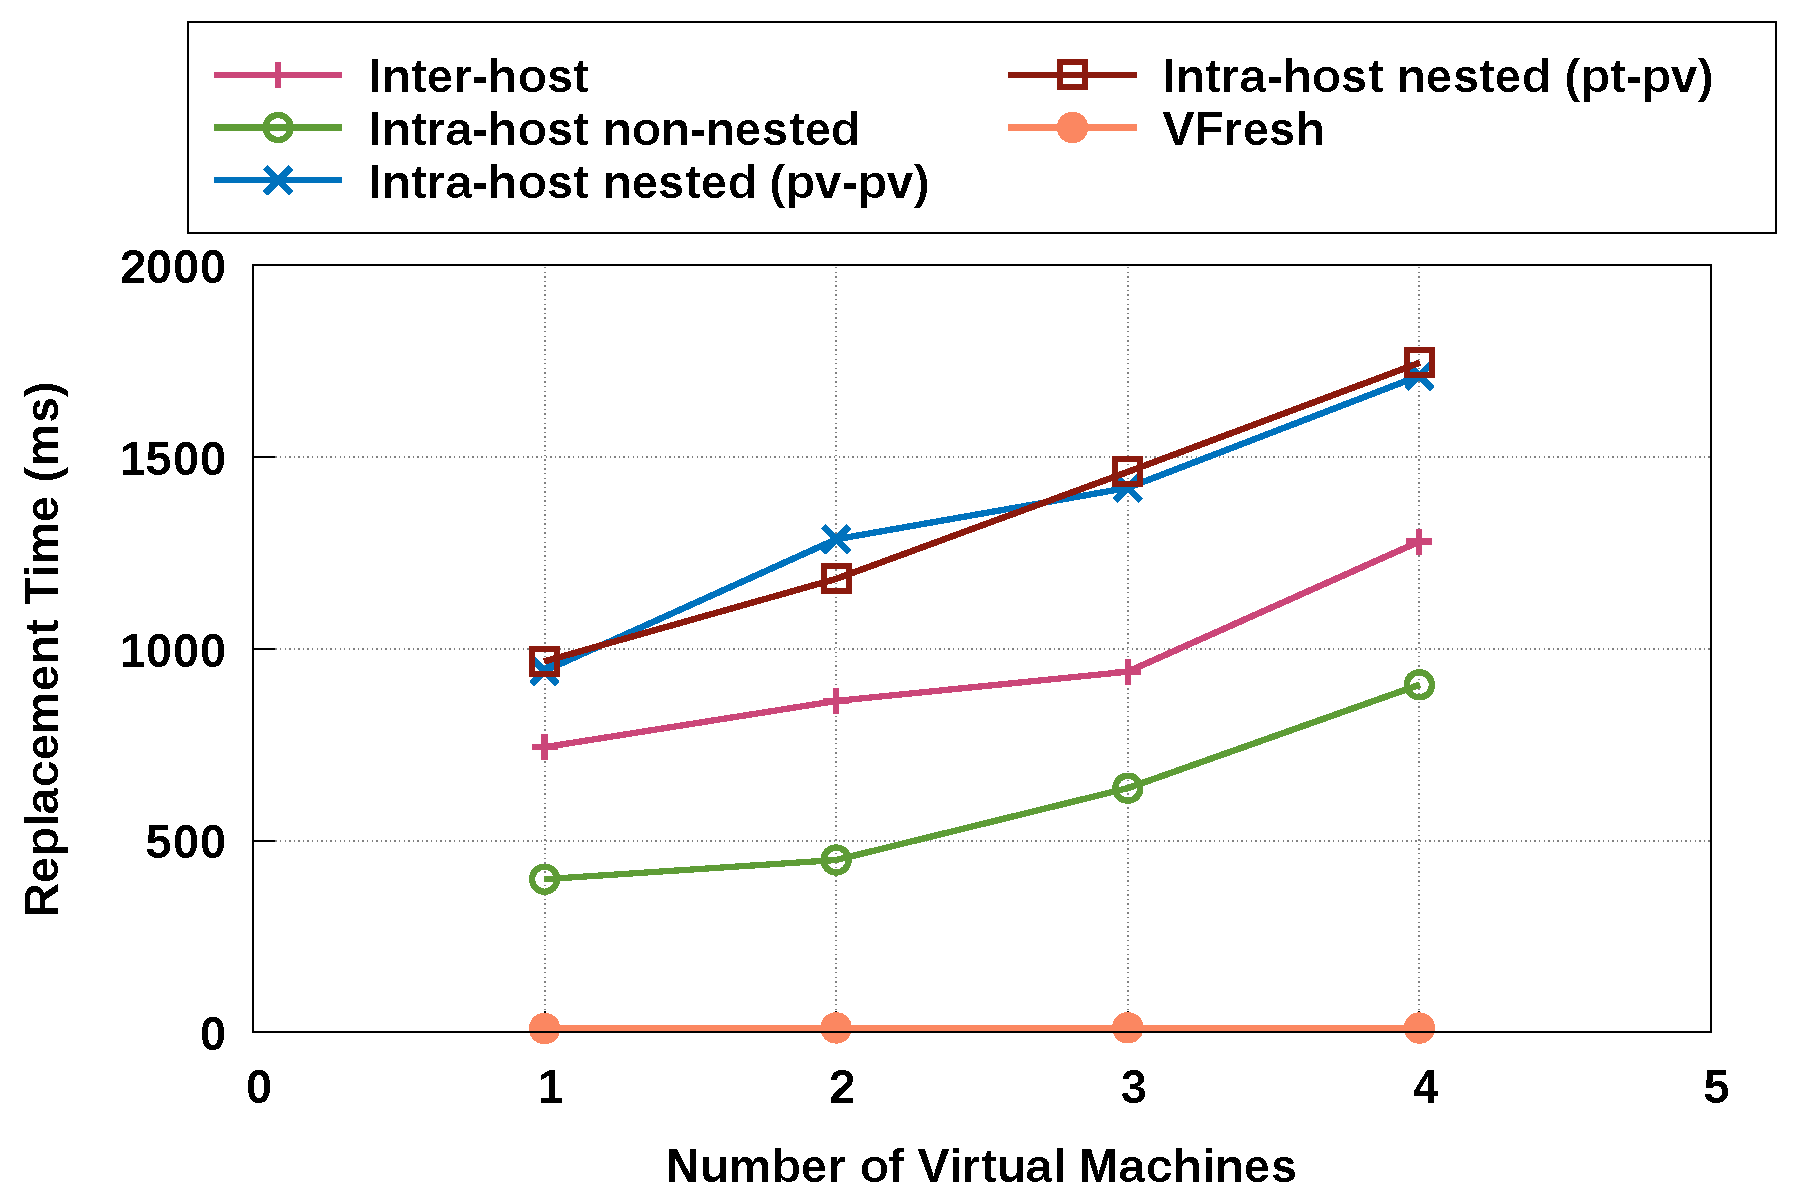
\includegraphics[width=0.45\textwidth]{figures/multivm_busy_guest_migration_vFresh.pdf}
%  \caption{Comparison of hypervisor replacement time for mutiple VMs running write-intensive workloads with \arch and different setups.}
%  \label{fig:multiVfreshBusy}
%\end{figure}

\begin{table}
\small
\begin{tabular}{|p{1.75cm}|p{1.85cm}|p{1.85cm}|p{1.5cm}|} \hline
 & Hyperplexor & Hypervisor & Guest \\ \hline
Host & 8GB, \linebreak 2CPUs & - & - \\ \hline
Non-Nested & 16GB, \linebreak 8CPUs & - & 8GB, \linebreak 2VCPUs \\ \hline
Nested & 32GB,  \linebreak 10CPUs & 16GB, \linebreak 8VCPUs & 8GB, \linebreak 2VCPUs \\ \hline
\arch & 32GB,  \linebreak 10CPUs & 16GB, \linebreak 8VCPUs & 8GB, \linebreak 2VCPUs \\ \hline
\end{tabular}
\raggedright The VM is configured with 4 VCPUs for iperf experiments. The host is also configured with 4 CPUs when iperf is run in host.
\vspace{6pt}
\caption{Experiment setup to measure the performance of Quicksort, Kernbench and iperf benchmarks in the guest.}
\label{tbl:configPerf}
\end{table}

\begin{figure*}
	\centering
    \subfloat[iperf]{
		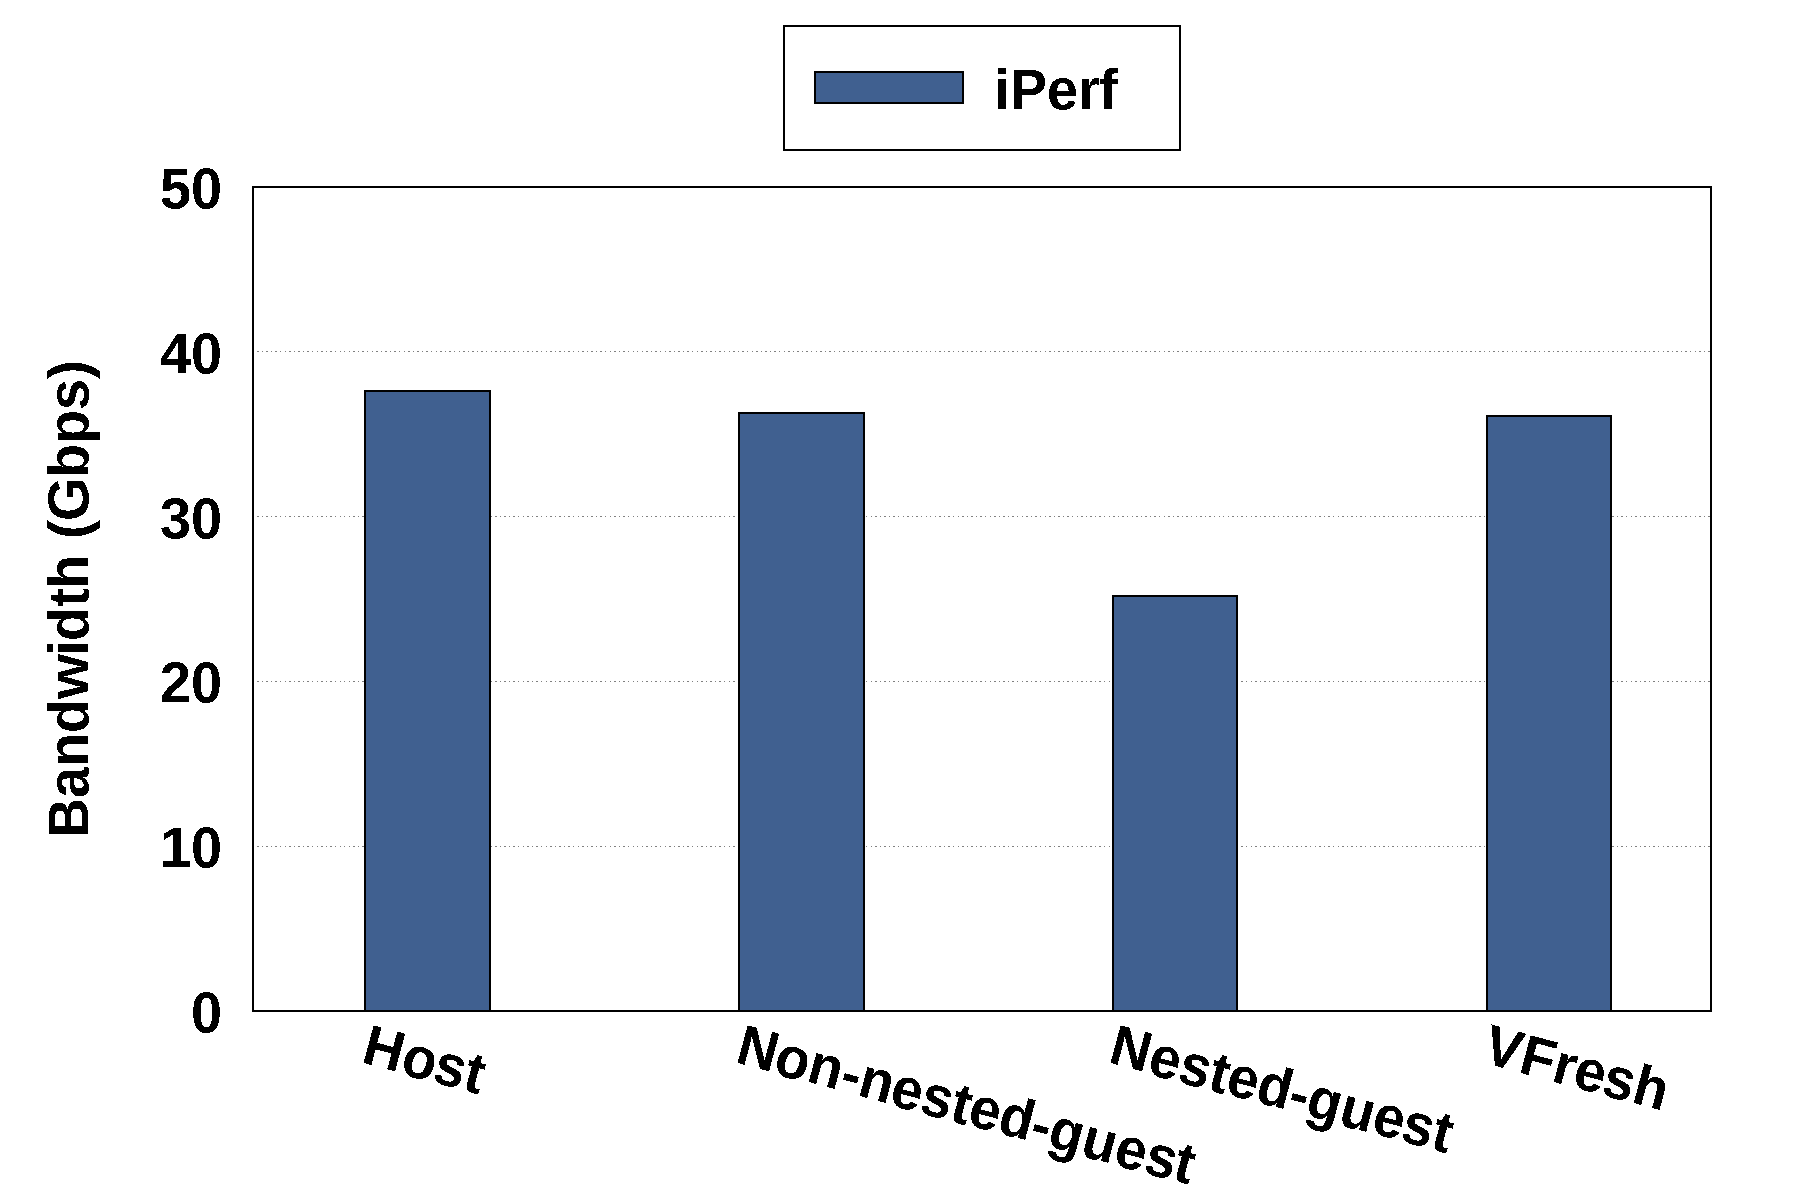
\includegraphics[width=.30\textwidth]{figures/iperf_vFresh.pdf}}
		\hspace{0.1in}
    \subfloat[Kernbench]{
		\includegraphics[width=.30\textwidth]{figures/kernbench_vFresh.pdf}}
		\hspace{0.1in}
	\subfloat[Quicksort]{
		\includegraphics[width=.30\textwidth]{figures/quicksort_vFresh.pdf}}
		%\hspace{0.1in}
    %\subfloat[Breakdown of CPU utilization in system, user modes and guest for iperf benchmark.]{
	%	\includegraphics[width=.22\textwidth]{figures/cpu_util_iperf.pdf}}
		%\hspace{0.1in}
		\vspace{-0.1in}
	\caption{Comparison of bandwidth, execution time and CPU utilization on hyperplexor with VFresh and different setups.}
	\vspace{-0.05in}
	\label{fig:impl}
\end{figure*}

\begin{figure}[t!]
  \includegraphics[width=0.33\textwidth]{figures/cpu_util_iperf.pdf}
  \caption{Breakdown of CPU utilization in system, user and guest modes for iperf benchmark.}
  \label{fig:cpuut}
\end{figure}

\subsubsection{Nesting Overhead Mitigation}
To demonstrate the benefits brought by \arch's optimizations to mitigate nesting overhead, we measure the performance of various applications running on (a) the native host (i.e., without virtualization), (b) a VM under non-nested virtualization (with the para-virtualized driver); (c) an L2 VM under nested virtualization (with the pt-pv configuration), and (d) an L2 VM under \arch with optimizations. The configurations for the experiments are listed in Table \ref{tbl:configPerf}. Particularly, to conduct fair comparisons among the above four cases, we ensure that the host or VMs running applications are configured with the same amount of resources --- 2 VCPUs and 8 GB memory. 
%The  performance is measured by running one of the following benchmarks. 
%\begin{itemize}

%\item \textbf{\textit{iPerf}} \cite{iperf} 
\para{Iperf} \cite{iperf} is used to measure network performance. We run the iperf client on the native host or VM under test, and the iperf server on a separate host (with sufficient resources). The iperf client and server are connected via a 40Gbps network. We measure the averaged TCP throughput over 100 seconds. 
%The CPU utilization is further broken down into the user mode, system mode
%due to the network workload in guest.

In \fref{fig:impl}a, we observe that under \arch (with optimizations) the performance of iperf is higher than the default nested case without optimizations, and very close to the non-nested case (under single-level virtualization). 

We also measure the CPU utilization in the hyperplexor, hypervisor and VM, respectively. \fref{fig:cpuut} shows the CPU utilization breakdown in the user mode, system mode the guest (VM) mode. Notice that, the CPU utilization in the user mode also includes the CPU consumed by the VM, while the CPU utilization in the system mode includes the CPU consumed by the hyperplexor (or the native host).

In the default nested case, when the NIC card is assigned to the hypervisor directly (i.e., pass-through), the CPU utilization of the hyperplexor is expected to be small, as the network packets are directly delivered to the L1 hypervisor. However, \fref{fig:cpuut} shows that the CPU utilization of the hyperplexor (i.e., the system mode) in the default nested case is very high. It is because, the hyperplexor burns CPU cycles when it executes HLT instruction as stated in Section \ref{sec:overhead}. In contrast, \arch reduces the CPU utilization of the hyperplexor by disabling \texttt{halt\_poll\_ns}. In consequence, the L1 hypervisor utilizes the CPU more in the VM mode, leading to higher iperf performance than the default nested case. 

%compared to the system mode in hyperplexor.   

%we measure the CPU utilization in hyperplexor while running iperf benchmark in guest. We measure the CPU consumed in user mode, system mode and by the guest separately. 
%The CPU utilization in user mode also includes the CPU consumed by the guest. 
%For a non-nested guest using para-virtual driver, more time is spent in the system to handle the network packets. As a result, the CPU utilization in system mode is high compared to user mode. 
%The CPU utilization of guest is almost equal to the user CPU utilization indicating that the guest is utilizing the CPU for the rest of the time. 
%When NIC card is assigned to the hypervisor, the CPU utilization in the hyperplexor is expected to be less as the network packets are directly delivered to the hypervisor. But the CPU utilization in hyperplexor is high as the hypervisor VCPUs burn CPU cycles when they execute HLT instruction. The nested guest uses para-virtual driver to handle the network traffic. The CPU utilization in the system mode in the hypervisor is higher than the CPU utilization in guest or user mode. In VFresh, we reduce the CPU utilization in system mode in hyperplexor by disabling halt\_poll\_ns. As seen from the results, the hypervisor now utilizes the CPU more in guest mode compared to the system mode in hyperplexor.   


%\item \textbf{\textit{Kernbench}} 
\para{Kernbench} \cite{kernbench} is a CPU and I/O intensive benchmark, which uses multiple threads to compile the kernel source code. More specifically, the benchmark fetches kernel source code files from disk for compilation and writes the binary files back after compilation. For our experiments, the kernel is compiled for five iterations and the number of threads used to perform kernel compilation is set to 2, equal to the number of VM VCPUs. 

In \fref{fig:impl}b, the non-nested VM brings 2.8\% performance overhead in comparison with the native case due to the single-level virtualization overhead; the default nested VM introduces 8.1\% overhead in comparison with the native case due to the additional layer in nested virtualization. %why 
\arch slightly reduces the overhead by 6\% and consumes less CPU in comparison with the default nested case.

\para{Quicksort} is a memory and CPU-intensive benchmark, as stated above. In \fref{fig:impl}c, the non-nested VM introduces only 0.3\% performance overhead in comparison with the native case; the default nested VM introduces 2.23\% overhead in comparison with the native case. %why 
Again, \arch slightly reduces the overhead by 15\% and consumes less CPU utilization in comparison with the default nested case.

%quicksort benchmarks causes overhead of 7.6\% and 1.9\% for kernbench and quicksort respectively, which do not show significant improvement. However, the performance does not degrade due to the optimizations applied. 

%\item \textbf{\textit{Quicksort}} 
%\para{Quicksort} \cite{williams2016enabling} is a memory and CPU-intensive benchmark. In the first stage, Quicksort allocates 1GB memory using malloc() system call. In the second stage, it writes random integers in the allocated memory and performs sorting operations using quicksort algorithm. In our experiments we measure the total number of sorting operations per second.


%\begin{table*}\centering
%\begin{tabular}{|p{4.5cm}|p{0.8cm}|p{0.8cm}|p{0.8cm}|p{0.8cm}|p{0.8cm}|p{0.8cm}|p{0.8cm}|p{0.8cm}|p{0.8cm}|p{0.8cm}|} \hline
%    \multirow{1}{*}{} & &
%      \multicolumn{9}{c|}{CPU Utilization} \\ \cline{3-11}
%    \multirow{1}{*}{} & Guest &
%      \multicolumn{3}{c|}{Hyperplexor} & 
%      \multicolumn{3}{c|}{Hypervisor} & 
%      \multicolumn{3}{c|}{Guest} \\ \cline{3-11}
 %& \multicolumn{9}{|c|}{\textbf{CPU Utilization (\%)}} \\ \cline{2-10}
 %& \multicolumn{3}{|c|}{\textbf{Host (\%)}} \\ \cline{2-4} 
% \multicolumn{3}{|c|}{\textbf{L1 (\%)}} \\ \cline{5-7}
% \multicolumn{3}{|c|}{\textbf{Guest (\%)}} \\ \cline{8-10}
% & \textbf{CPU Utilization on Host (\%)} \\ \hline
%\textbf{} & & User & System & Guest & User & System & Guest & User & System & Guest \\ \hline
%\multirow{ 2}{5cm}{Non-nested guest (pv)} & Server & 114.63 & 247.09 & 114.63 & - & - & - & 1.8 & 91.7 & 0 \\ 
%& Client & 114.4 & 122.7 & 114.3 & - & - & - & 1.18 & 84.64 & 0 \\ \hline

%\multirow{ 2}{5cm}{Nested Guest (pt-pv)} & Server & 253.1 & 308.3 & 252.9 & 91.18 & 150.72 & 90.9 & 1.9 & 107.18 & 0\\ 
%& Client & 126.3 & 205.7 & 126.5 & 82.72 & 107.54 & 82.63 & 0.63 & 121.17 & 0 \\ \hline

%\multirow{ 2}{5cm}{\arch} & Server & 265.7 & 85.5 & 265.7 & 116.2 & 143.1 & 116.45 & 2.45 & 118.44 & 0 \\ 
%& Client & 195.6 & 93.5 & 195.6 & 95.54 & 93.18 & 95.27 & 1.17 & 135.8 & 0 \\ \hline

%\end{tabular}
%\vspace{6pt}
%\caption{CPU Utilization: }
%\label{tab:cpuut}
%\end{table*}


%Fig.11 c explanation
%In our experiments, we disable the halt_poll_ns parameter.  In nested virtualization experiments, mainly network experiments (iperf), we assign 8 vCPUs to L1 hypervisor and 4 vCPUs to L2 guest and the host has 10CPUs. As we isolate and pin L1 vCPUs to pCPUs, 8 pCPUs are occupied and other 2 pCPUs are dedicated for QEMU and other I/O threads associated with QEMU. When the interrupt has to be delivered to L2 guest vCPUs, L2 has to be scheduled on pCPUs first, by pre-empting L1 vCPU on which it was running. If halt_poll_ns is 0, L1 vCPU will execute HLT instruction faster and the L0 scheduler schedules L2 vCPU and interrupt gets delivered faster. 
%That way, the network performance becomes better in our solution using nested virtualization.

%KERNBENCH
%host - 2 CPUs, 8G
%37.47
%single-level, vhost-net , 8 CPUs, 2 vCPUs, 16G, 8G
%38.51
%nested, passthrough-vhost, 10CPUs, 8vCPUs, 2 vCPUs
%40.524
%VFresh
%40.324

%CPU Utilization
%host - 155.95
%single-level - 170.12
%nested, passthrough-vhost - 168.7
%VFresh - 168.5

%QUICKSORT
%host - 2 CPUs, 8G
%66.29
%single-level, vhost-net , 8 CPUs, 2 vCPUs, 16G, 8G
%66.51
%nested, passthrough-vhost, 10CPUs, 8vCPUs, 2 vCPUs
%67.77
%VFresh
%67.57

%CPU Utilization
%host - 97.71
%single-level - 102.1
%nested, passthrough-vhost - 99.4
%VFresh - 97.5

%IPERF
%host - 2 CPUs, 8G
%SENDER: 37.6 Gbps RECEIVER: 37.6 Gbps
%single-level, vhost-net , 8 CPUs, 2 vCPUs, 16G, 8G
%SENDER: 36.3 Gbps RECEIVER: 29.9 Gbps
%nested, passthrough-vhost, 10CPUs, 8vCPUs, 2 vCPUs
%SENDER: 25.2 Gbps RECEIVER: 26.6 Gbps
%nested, passthrough-vhost, 10CPUs, 8vCPUs, 2 vCPUs + optimizations

%\end{itemize}

%In Table 1 we measure the performance overhead caused due to virtualization. We compare the overhead caused due to nested virtualization with non-nested virtualization. In our proposed solution we measure the performance by applying the following optimizations for nested case. The 8 VCPUs of hypervisor are pinned to 8 CPUs, CPUs are isolated so that any other process other than VCPU does not get scheduled on CPU. 1 CPU is dedicated to schedule hypervisor and QEMU threads.The NIC card is directly assigned to hypervisor and halt\_poll\_ns is set to zero in hyperplexor. For nested case, we passthrough the NIC card to hypervisor and the guest uses para-virtualized driver.

%In \fref{fig:impl} (b), for non-nested guest, to measure the iperf performance the guest is configured with para-virtualized driver. 
%The performance of iperf is 36.3 Gbps for a 40 Gbps NIC card when iperf client is run in guest. However, the performance reduces to 29.9 Gbps when iperf server is run in the guest. The loss in performance is due to the processing of huge number of incoming packets. When iperf is run in nested guest the performance reduces to 25.2 Gbps. %why
%In our solution, as the halt\_poll\_ns is disabled in the hyperplexor, the CPU scheduler gets invoked and schedules the nested guest VCPUs sooner to handle the interrupts. As a result the performance of iperf is now comparable with the performance in the single-level guest.

%\begin{figure}[t!]
%  \includegraphics[width=0.45\textwidth]{figures/cpu_util_iperf.pdf}
%  \caption{Breakdown of CPU utilization in system, user modes and guest for iperf benchmark.}
%  \label{fig:cpuut}
%\end{figure}


%The performance of kernbench and quicksort introduces 2.8\% and 0.3\% overhead respectively in non-nested guest compared to host, whereas the nested guest introduces 8.1\% and 2.23\% overhead due to the additional layer of virtualization. %why 
%With our proposed solution the performance of kernbench and quicksort benchmarks causes overhead of 7.6\% and 1.9\% for kernbench and quicksort respectively, which do not show significant improvement. However, the performance does not degrade due to the optimizations applied. 


%\begin{figure} 
%	\centering
%	\includegraphics[width=0.5\textwidth]{figures/space_used.eps}
%	\caption{Space Used For Migration}
%	\label{fig: spaceused}
%\end{figure}

\subsection{OS Replacement}
%\subsubsection{OS Replacement}
We run our experiments on a server machine equipped with two 6-core Intel Xeon CPUs of 2.1 GHz and 128 GB memory. We use KVM/QEMU to run source and destination VMs on the same server host. Both VMs are configured with 4 VCPUs and 4 GB memory. \arch's OS replacement is implemented with CRIU version 3.5. 
%Table \ref{tab:experiment1}. shows the configuration of the hyperplexor and the VMs.

\begin{figure}
	\centering
	\subfloat[Replacement time]{
		\includegraphics[width=.235\textwidth]{figures/memory_dirty_rate_process_migration_tmt.pdf}}
	\subfloat[Frozen time]{
		\includegraphics[width=.235\textwidth]{figures/memory_dirty_rate_process_migration_tft.pdf}}
	\caption{Effect of memory intensive workload on OS replacement.}
	\label{fig:variation23}
    \vspace{0.2in}
\end{figure}

\begin{figure*}
	\centering
    \subfloat[Sysbench]{
		\includegraphics[width=.24\textwidth]{figures/sysbench_performance.pdf}}
		%\hspace{0.1in}
	\subfloat[Parsec]{
		\includegraphics[width=.328\textwidth]{figures/parsec.pdf}}
		\hspace{-0.1in}
    \subfloat[Quicksort]{
		\includegraphics[width=.42\textwidth]{figures/quicksort_performance.pdf}}
	%\hspace{0.1in}
		%\vspace{-0.1in}
	\caption{Comparison of application performance for OS replacement.}
	%\vspace{-0.1in}
	\label{fig:impl1}
\end{figure*}
%\begin{table}
%	\begin{tabular}{|c|c|c|}
%		\hline
%		 Hyperplexor & VM (stale OS) & VM (replacement OS) \\
%		\hline
%		128GB, 12 CPUs    & 4GB, 4 VCPUs    & 4GB, 4 VCPUs \\
%		\hline
%	\end{tabular}
%	
%	\caption{Setup for OS replacement experiments}
%	\label{tab:experiment1}
%\end{table}

\subsubsection{Replacement Time}
We measure the OS replacement time under \arch and compare it with the pre-copy live migration approach (implemented based on PHaul \cite{phaul}). We run a container with one process which allocates 1 GB memory and then continuously performs write operations to the memory pages at varying rates from 0 MB/second (i.e., no dirty pages) to 1 GB/second (i.e., all pages are dirtied each second). We compare the total OS replacement time and the container downtime (i.e., frozen time).

\fref{fig:variation23} shows that, with the pre-copy live migration approach the total OS replacement time and the frozen time increase as the memory dirty rate increases. For example, the replacement time is around 2.5 seconds when the dirty rate is 0, and increases to 10 seconds when the dirty rate is 1 GB/second. The frozen time is around 1.7 seconds when the dirty rate is 0, and increases to 2.7 seconds when the dirty rate is 1 GB/second. In contrast, with \arch, the total replacement time and frozen time remain constant, around 0.5 seconds (i.e., the total replacement time equals to the frozen time in \arch). Because \arch transfers the memory ownership instead of copying memory pages, it leads to much shorter OS replacement time and frozen time compared with the pre-copy based approach. 

We notice that the OS replacement time (0.5 seconds with 1 GB memory) is higher than the hypervisor replacement time (e.g., 10 ms). The main reason is that, \arch's OS replacement builds on a popular user space checkpointing/restoration tool (i.e., CRIU), which incurs high overhead in collecting state of processes during which processes are paused. A low-overhead, kernel-level solution is a subject of our ongoing investigations.

%the effect of container's memory usage on the OS replacement time. We start a container with memory intensive processes which allocate 1 GB memory and perform a continuous write operation on it at a varying rate ranging from 0MB/second to 1GB/second. We compare the OS replacement time of VFresh with CRIU. To complete the OS replacement, CRIU takes multiple iterations to send all the memory state. With increase in memory writing rate, memory getting dirtied during each iteration increases. Hence, the replacement time and the downtime increases as well. Additionally, if the iterations are not stopped manually, then the replacement operation will never complete, reason being the size of the dirtied memory during the iterations is not converging. However, OS replacement and downtime using \arch stay not only very small compared to CRIU, but also constant with variation in memory writing rate. Since VFresh is not iterative and the total memory usage is constant, so the replacement time doesn't get affected by the change in memory writing rate. 



\subsubsection{Performance Impact}
\label{sec:workload}

We use the following three macro-benchmarks to show performance impact during OS replacement.

\para{Sysbench} \cite{sysbench} provides multi-threaded memory testing by reading from or writing to preallocated memory. In our experiments, we preallocate a buffer with varying sizes from 128 MB to 1 GB, and perform write operations to this buffer repetitively till its completion --- a total size of memory has been written (i.e., 1,000 GB in our experiments). We compare three cases: (a) the baseline without OS replacement; (b) pre-copy based approach using CRIU; and (c) \arch. In cases (b) and (c), we conduct one OS replacement during each run.

%We use this benchmark to show the total completion time of a write-intensive experiment.

In Figure \ref{fig:impl1}a, the completion time under \arch is almost the same as the baseline (without OS replacement). On the contrary, the pre-copy based approach takes longer time to complete for each run. Further, the completion time increases as the buffer size increases --- the large the buffer size, the more memory pages needed to be copied for the pre-copy based approach. 
%the completion time
%we compare the sysbench completion time while changing the buffer size from 128MB to 1024MB. The baseline data represents the completion time of sysbench a VM. To compare with this baseline data, we migrate a running sysbench application and observe its completion time after migration. Performance of sysbench with migration using \arch is almost similar to baseline. However, sysbench takes much longer time to complete when migrated using CRIU. Furthermore, its completion time using CRIU increases more rapidly with the increment in buffer size. In \arch the change in completion time is not significant.

\para{Parsec} \cite{parsec} benchmark mimics large-scale commercial applications. We run a variety of sub workloads of parsec benchmark, during which we perform OS replacement. As each workload takes a long time to complete, we compare the total frozen time during the OS replacement between \arch and the pre-copy based approach.


\fref{fig:impl1}b shows that the total frozen time for workloads with higher memory usage is longer than workloads with lower memory usage. For example, canneal and fluidanimate have very high memory usage, whereas swaptions and bodytrack use only a small amount of memory. Hence, canneal and fluidanimate have longer frozen time during the OS replacement than swaptions and bodytrack. Yet, the total frozen time of all the workloads with \arch is almost half the size of that with the pre-copy based approach.
%Figure \ref{fig:impl1} (b) compares the total frozen time of different workloads of parsec benchmark while being migrated using \arch and CRIU. We have used workloads with varying memory usage. We observe that the total frozen time for workloads with high memory usage is higher compared to workloads with lower memory usage. For example, canneal and fluidanimate workload have very high memory usage whereas swaptions and bodytrack use only a small amount of memory. Hence, canneal and fluidanimate workloads are frozen longer during migration compared to swaptions and bodytrack. However, the total frozen time of the workloads using \arch is almost half compared to CRIU.

\para{Quicksort} is used again to show the number of quicksort operations per second, when we conduct multiple OS replacements. Figure \ref{fig:impl1}c shows that, the number of quicksort operations per second during OS replacement reduces to zero for a short period of time with the pre-copy based approach. In contrast, with \arch, we observe at least 200$\sim$400 quicksort operations per second during the OS replacement. This is because, the frozen time with \arch is much smaller than that with the pre-copy based approach.

%\begin{figure*}
%	\centering
%	
%	\subfloat[Total Migration Time]{
%		\includegraphics[width=.5\textwidth]{figures/memory_usage_process_migration_tmt.pdf}}
%	\subfloat[Total Frozen Time]{
%		\includegraphics[width=.5\textwidth]{figures/memory_usage_process_migration_tft.pdf}}
%	\caption{Memory Size Variations}
%	\label{fig:variation1}
%\end{figure*}
%\begin{figure*}
%	\centering
	
%	\subfloat[Total Migration Time]{
%		\includegraphics[width=.5\textwidth]{figures/memory_dirty_rate_process_migration_tmt.pdf}}
%	\subfloat[Total Frozen Time]{
%		\includegraphics[width=.5\textwidth]{figures/memory_dirty_rate_process_migration_tft.pdf}}
%	\caption{Memory Dirtying Rate Variations}
%	\label{fig:variation1}
%\end{figure*}

%%%%%%%%% DATA for Figure 12 a %%%%%%%%
%		Vfresh	CRIU
%0		0.571	2.56
%250	0.587	5.87
%500	0.591	7.19
%750	0.566	8.58
%1000	0.532	10.23

%%%%%%%%% DATA for Figure 12 b %%%%%%%%
%		Vfresh	CRIU
%0		0.567	1.308
%250	0.581	1.75
%500	0.585	1.98
%750	0.561	2.29
%1000	0.527	2.67

%\begin{figure}
%	\centering
%	
%	\subfloat[Total Migration Time]{
%		\includegraphics[width=.25\textwidth]{figures/busy_process_migration.pdf}}
%	\subfloat[Total Frozen Time]{
%		\includegraphics[width=.25\textwidth]{figures/total_mem_usage_TFT.eps}}
%	\caption{Memory Size Variations}
%	\label{fig:variation1}
%\end{figure}
%\begin{figure}
%	\centering
%	
%	\subfloat[Total Migration Time]{
%		\includegraphics[width=.25\textwidth]{figures/memory_dirtying_TMT.eps}}
%	\subfloat[Total Frozen Time]{
%		\includegraphics[width=.25\textwidth]{figures/memory_dirtying_TFT.eps}}
%	\caption{Memory Dirtying Rate Variations}
%	\label{fig:variation2}
%\end{figure}

%Figure \ref{fig:variation1} shows the total migration time and the total frozen time of a process that is using varying size of the memory. Our starting point is a process using minimal memory and then we increase the memory usage to see the effect of the total memory size on the total migration time and total frozen time.









%\begin{figure} 
%	\centering
%	\includegraphics[width=0.5\textwidth]{figures/comapped_bk.eps}
%	\caption{mWarp's Total Frozen Time Breakdown}
%	\label{fig: breakdown2}
%\end{figure}

%We consider the case, where we allocate 1GB and dirties it at 1GB per second continuously, to show the breakdown of the total frozen time during the migration. Figure \ref{fig: breakdown2} show migration causes downtime in the execution of the process during checkpointing, moving the other states and restoration. 


%\begin{figure*}
%	\centering
%	\subfloat[Frozen time breakdown during checkpointing.]{
%		\includegraphics[width=.5\textwidth]{figures/comapped_chkpnt_bk.eps}}
%		\hspace{0.1in}
%	\subfloat[Frozen time breakdown during restoration.]{
%		\includegraphics[width=.450\textwidth]{figures/comapped_rst_bk.eps}}
%		%\hspace{0.1in}
%		\vspace{-0.1in}
%	\caption{mWarp's Frozen Time Breakdown During Migration Stages}
%	\vspace{-0.2in}
%	\label{fig: breakdown3}
%\end{figure*}

%Figure \ref{fig: breakdown3} shows the further breakdown of the frozen time during the checkpointing and restoration stage.
%\begin{figure} 
%	\centering
%	\includegraphics[width=0.45\textwidth]{Figures/quicksort_per_sec.eps}
%	\caption{Quicksort Rate}
%	\label{fig: quicksort}
%\end{figure}

%\begin{figure} 
%	\centering
%	\includegraphics[width=0.5\textwidth]{figures/quicksort_performance.pdf}
%	\caption{Quicksort's Performance}
%	\label{fig: quicksort1}
%\end{figure}

%%%%%%%%% DATA for Figure 13 a %%%%%%%%
%		Baseline VFresh	CRIU
%128	10.014	10.0992	10.6237
%256	10.0366	10.283	11.1255
%512	10.0514	10.4231	11.375
%1024	10.1504	10.4893	12.6827
%%%%%%%%% DATA for Figure 13 b %%%%%%%%
%		VFresh	CRIU
%CN		0.912	2.09
%BS		0.458	1.194
%FQ		0.474	0.86
%FA		0.601	1.561
%SP		0.325	0.626
%BT		0.296	0.575



%\begin{figure*}[t!]
% 	  \includegraphics[width=0.98\textwidth]{figures/migration.pdf}
%  \caption{Architecture for hypervisor replacement with direct-device assignment and thin hyperplexor.}
%TODO: Please fix this caption
 % \label{fig:vFresharch}
  %\includegraphics[width=15cm,height=6cm,keepaspectratio]{architecture__1_.jpg}
%\end{figure*}


%\begin{figure} 
%	\centering
%	\includegraphics[width=0.5\textwidth]{figures/sysbench_performance.pdf}
%	\caption{Sysbench Performance}
%	\label{fig: sysbench}
%\end{figure}

%\begin{figure} 
%	\centering
%	\includegraphics[width=0.5\textwidth]{figures/parsec.pdf}
%	\caption{Downtime Of Parsec Workloads}
%	\label{fig: parsec}
%\end{figure}



\section{Related Work}




%%%%%%%%%%%%%%%%%%%%%%%%%%%%%%%%%%%%%%%%%%%5
%\begin{figure}[t!]
%  \includegraphics[width=0.5\textwidth]%{figures/qsortps_1GB_nested_precopy_disable_rate_limit.pdf}
  %\caption{Performance of QuickSort }
  %\label{quicksort-performance-1GB-nested-vhost-vhost.png}
%\end{figure}

%\begin{figure}[t!]
%  \includegraphics[width=0.35\textwidth]{figures/qsortps_1GB_nested_precopy_hyperfresh.pdf}
  %\caption{Performance of QuickSort during migration of a nested guest}
%  \label{quicksort-performance-1GB-nested-vhost-vhost.png}
%\end{figure}

%\begin{table*}\centering

%\begin{tabular}
%{|p{4cm}|p{1cm}|p{1cm}|p{1.5cm}|p{1.5cm}|p{1.5cm}|p{1.5cm}|p{1.5cm}|} \hline
% & & & & & \multicolumn{3}{c|}{\% Overhead vs. Host} \\ \cline{6-8} 
%Benchmark & Host & Non-nested Guest & Nested Guest & Our Solution & Non-nested Guest & Nested %Guest & Our Solution \\ \hline
%iPerf Bandwidth (Gbps) - Server & 37.6 & 29.9 & 25.2 & 29.7 & 20.5 & 32.97 & 21 \\ 
%iPerf Bandwidth (Gbps) - Client & 37.6 & 36.3 & 26.6 & 36.1 & 3.45 & 29.25 & 3.98 \\ \hline
%Kernbench Runtime (seconds) & 37.47 & 38.51 & 40.52 & 40.32 & 2.8 & 8.1 & 7.6 \\ \hline
%Quicksort Runtime (useconds) & 66.29 & 66.51 & 67.77 & 67.57 & 0.3 & 2.23 & 1.9 \\ \hline
%
%\end{tabular}
%\vspace{6pt}
%
%\caption{Comparison of performance overhead due to virtualization}
%\label{Comparison of performance overhead due to virtualization}
%\end{table*}

%\begin{table*}\centering
%\begin{tabular}{|p{4.5cm}|p{0.8cm}|p{0.8cm}|p{0.8cm}|p{0.8cm}|p{0.8cm}|p{0.8cm}|p{0.8cm}|p{0.8cm}|p{0.8cm}|p{0.8cm}|} \hline
%    \multirow{1}{*}{} & &
%      \multicolumn{9}{c|}{CPU Utilization} \\ \cline{3-11}
%    \multirow{1}{*}{} & Guest &
%      \multicolumn{3}{c|}{Hyperplexor} & 
%      \multicolumn{3}{c|}{Hypervisor} & 
%      \multicolumn{3}{c|}{Guest} \\ \cline{3-11}
 
%\textbf{} & & User & System & Guest & User & System & Guest & User & System & Guest \\ \hline
%\multirow{ 2}{5cm}{Non-nested guest (paravirt)} & Server & 114.63 & 247.09 & 114.63 & - & - & - & 1.8 & 91.7 & 0 \\ 
%& Client & 114.4 & 122.7 & 114.3 & - & - & - & 1.18 & 84.64 & 0 \\ \hline

%\multirow{ 2}{5cm}{Nested Guest (passthrough-paravirt)} & Server & 253.1 & 308.3 & 252.9 & 91.18 & 150.72 & 90.9 & 1.9 & 107.18 & 0\\ 
%& Client & 126.3 & 205.7 & 126.5 & 82.72 & 107.54 & 82.63 & 0.63 & 121.17 & 0 \\ \hline

%\multirow{ 2}{5cm}{Nested Guest (passthrough-paravirt) + Optimizations} & Server & 265.7 & 85.5 & 265.7 & 116.2 & 143.1 & 116.45 & 2.45 & 118.44 & 0 \\ 
%& Client & 195.6 & 93.5 & 195.6 & 95.54 & 93.18 & 95.27 & 1.17 & 135.8 & 0 \\ \hline

%\end{tabular}
%\vspace{6pt}
%\caption{CPU Utilization}
%\label{CPU Utilization}
%\end{table*}


%\begin{table}
%\begin{tabular}{|p{3.2cm}|p{2.0cm}|p{2.0cm}|} \hline
% & \multicolumn{2}{|c|}{\textbf{Number of VM Exits}} \\ \cline{2-3} 
%\textbf{VM Exit Reasons}& \textbf{Before optimizations} & \textbf{After optimizations}\\ %\hline
%\textbf{HLT} & &\\ \hline
%\textbf{MSR\_WRITE} & &\\ \hline
%\textbf{EXTERNAL\_INTERRUPT} & &\\ \hline
%\textbf{PREEMPTION\_TIMER} & &\\ \hline
%\textbf{IO\_INSTRUCTION} & &\\ \hline
%\textbf{EXCEPTION\_NMI} & &\\ \hline
%\textbf{PAUSE\_INSTRUCTION} & &\\ \hline
%\textbf{EPT\_VIOLATION} & &\\ \hline
%\textbf{MSR\_READ} & &\\ \hline
%\textbf{CPUID} & &\\ \hline
%\textbf{TOTAL} &  &\\ \hline
%\end{tabular}
%\vspace{6pt}
%\caption{VM Exit Reasons}
%\label{VM Exit Reasons}
%\end{table}
 
%\begin{document}

Software aging \cite{parnas1994software} is the phenomenon where
software errors, such as  memory leaks, accumulate over time,
leading to performance degradation or complete system failure.
Software Rejuvenation \cite{huang1995software} is a proactive technique where 
the system is periodically restarted to a clean internal state to
counter software aging. In cloud environments, software aging 
of hypervisors and OS is of utmost concern, where the impact of 
their failures could be widespread.

In cold rejuvenation of hypervisors, all VMs must be restarted
whereas in warm rejuvenation the VMs' memory state is preserved 
in persistent memory and restored after hypervisor rejuvenation, 
avoiding costly read/writes to persistent storage. 
Roothammer \cite{kourai2007fast} proposed warm reboot to rejuvenate 
a Xen hypervisor 
%which avoids cache-misses by preserving the 
VM images in main memory reducing the VM reboot time. 

A simpler approach is to live migrate the VMs to a different host. 
Live migration~\cite{clark2005live, postcopy} reduces the downtime 
by letting the virtual machines run when the memory is copied in 
multiple rounds to another host. However, live migration also incurs 
network overhead as large quantities of memory is transferred. 
In this paper, we eliminate the memory copies for intra-host VM/container 
migration by page relocation on the same host. 
%We also eliminate multiple copies of VM images as the hypervisor replacement happens on the same machine. 
ReHype \cite{le2011rehype} performs a microreboot~\cite{candea2004microreboot} of 
the hypervisor by preserving the state of the VMs. The state of 
the rebooted hypervisor is then re-integrated with the state of the preserved VMs. 
Since this reintegration depends heavily on the hypervisor's state,
the success rate is low.   
Kourai et. al proposed VMBeam \cite{kourai2015zero}
where a clean virtualized system is started and all the 
virtual machines are migrated from old virtualized system to new one 
with zero-memory copy. Unlike our approach, VMBeam takes 16.5 seconds 
to migrate a 4 GB VM with zero memory copy, potentially due to 
non-live or inefficient transfer of memory maps. 
HyperFresh~\cite{hyperfresh_apsys} also uses memory co-mapping  to
replace a stale hypervisor with a fresh one. However, the refresh times 
are close to 100 ms for relocating a single VM, and multiple VMs relocation
is not addressed. Finally, unlike the above approaches, our \arch
addresses reduction of nesting overheads during normal execution
and live OS replacement for processes and containers.

%Remus \cite{cully2008remus} is a reactive technique that achieves high availability by periodically checkpointing the VM image and incrementally storing the changes in the memory of backup host. On failure of current host, the VM can be immediately started on the backup host using the checkpointed memory. The VM images along with network and disk state are checkpointed as frequently as 25ms. To transfer the incremental changes in the VM’s memory, it requires higher network bandwidth. The traffic generated over the network results in performance degradation of the applications running in the virtual machines. VMWareFT \cite{scales2010design} uses deterministic replay to keep both primary and backup VMs in sync. Again it requires high quality network connections. In our technique, we transfer only the processor and the I/O state during hypervisor replacement through the network. As shown in the evaluation section, it does not affect the performance of the applications running in the VM. Upon encountering an error in the hypervisor, 

Applying updates to an OS kernel comes with high cost of downtime due to system reboot. 
Kernel patching is a complex process of replacing original outdated functions or 
data structures with new ones. Ksplice \cite{arnold2009ksplice}, Kpatch \cite{kpatch1, kpatch2}, 
Kgraft \cite{kgraft} follow the mechanism of replacing old vulnerable functions with 
new functions using ftrace mechanism. Kpatch and Ksplice stop the machine to check 
if any of the threads is executing in the function to be patched. If any of the processes 
is executing or is sleeping in the function to be patched, the kernel patching is retried later 
or called off after several attempts. Kgraft keeps a copy of both old and new functions. 
If the kernel code is active during patching, it runs till completion before switching to 
the new functions while the other processes use the updated functions. 
Live patching \cite{livepatch} is a combination of Kpatch and Kgraft kernel patching 
methods. Kernel patching technique can be useful for applying simple 
fixes to delay system failure until the next maintenance period, 
but it still requires an OS reboot at some stage. 
Major changes to the kernel also require immediate reboot to take effect. 
Further these techniques cannot patch asm, vdso, or functions that cannot be traced.
In contrast, \arch bypasses these problems by remapping the memory of
containers/processes to a fresh co-located instance of the kernel.

Process/container live migration techniques have also been extensively studied 
\cite{spin, exokernel, synthetix, baraks, zayas, douglis, theimer, lsf, condor, criu},
but all require the transfer of the memory contents via network. 
\arch combines memory remapping with intra-host process migration used by CRIU~\cite{criu}
to eliminate memory copying, making it suitable for fast and live OS replacement.

%In general, process migration can be implemented either in the kernel level or in the user level. Kernel level process migration techniques \cite{spin, exokernel, synthetix, baraks, zayas, douglis, theimer} are implemented either with kernel-level inherent support or by modifying the existing operating systems adding complexity. In contrast, user-level implementation \cite{lsf, condor, criu, Amoeba, Chorus, Mach} requires either to modify applications reducing the transparency or to heavily intrude processes for collecting state facing performance degradation. The performance overhead of user-level implementations can be significantly mitigated with key kernel-level support such as exposing as much state information of processes as possible to the user space and/or providing efficient ways to mark dirty pages and transfer them \cite{condor, lsf, criu}. As a container consists of a hierarchy of processes as well as mechanisms that enable isolation and security between containers, state-of-the-art container migration approaches  \cite{docker, openvz, coreos_rocket} build upon process migration. For example, the migration of Docker container \cite{docker} builds on CRIU's \cite{criu} process checkpointing and restoring mechanisms. 

%\para{Live Migration.} A lot of live migration techniques have been proposed.  One approach is post-copy technique \cite{Hines:2009:PLM:1618525.1618528, zayas}, where pages are migrated only when they are referred on the destination machine. Although such an on-demand page migration reduces the initial cost of the migration, it increases the total migration time. Pre-copy \cite{theimer} keeps processes/containers running on the source machine while its memory keeps getting transferred to the destination in an iterative manner; once the dirtied pages are small enough, the whole process is paused and the remaining pages are transferred. If the page dirtying rate is very high, the migration will take way longer to complete. There has also been work that combines some features of these techniques \cite{lazo, loubutin, sinha, dediu, dijk,schill,petri,schrimpf} . For example, instead of copying entire memory state in the most basic technique, only the minimal dirty pages are transferred \cite{roush}. The remaining pages are transferred while the process is running on remote machine. This reduces the transfer cost, but requires the support of the remote paging mechanism. MOSIX \cite{mosix} and Sprite \cite{sprite} implements migration by leaving residual dependencies on the source machine. Although, it makes the migration simple but it requires the source machine to be available all the time till the process completes its execution. 


%\begin{figure}[t!]
%  \includegraphics[width=0.5\textwidth]{figures/quicksort.pdf}
%  \caption{Quicksort performance}
%\end{figure}

%\begin{figure}[t!]
%  \includegraphics[width=0.5\textwidth]{figures/kernbench.pdf}
%  \caption{Kernbench performance}
%\end{figure}

%\begin{figure}[t!]
%  \includegraphics[width=0.5\textwidth]{figures/iperf.pdf}
%  \caption{iPerf performance}
%\end{figure}


%SENDER: 36.1 Gbps RECEIVER: 29.7 Gbps

\vspace{-0.2in}
\section{Conclusion}
We have presented \arch, a faster and less disruptive live hypervisor replacement approach.
Leveraging nested virtualization, a thin hyperplexor transparently 
relocates the ownership of VMs' pages from the stale hypervisor to a new updated hypervisor on 
the same host, without memory copying overheads.
\arch also mitigates nesting overhead via direct device assignment, and other optimizations. 
We also demonstrate how hyperplexor-based remapping approach 
can be applied for live replacement of an 
operating system for containers/processes.
Evaluations of our \arch prototype implementation show sub-10ms hypervisor replacement
times for VMs and sub-second OS replacement times for containers.


%Hypervisors are tend to software aging and require frequent reboots. We show that pre-copy migration takes significant time to migrate VMs from one host to another and affect the performance of the applications running in the guest during migration. We propose a technique, \arch to replace the hypervisor without causing service disruption in the guest using nested virtualization to switch the old hypervisor by a healthy one. We co-map the memory of guest to avoid pre-copy memory iteration rounds and transfer only the VCPU and I/O state during migration and show that the hypervisor replacement time is within 10ms. The healthy hypervisor can be a patched hypervisor or a hypervisor with clean state. \arch achieves network performance in nested guest comparable to single-level guest by applying optimizations to hypervisor.


\bibliographystyle{plain}
\bibliography{bibliography/references}
\end{document}
